%=========================================
%  Concentric Radii Maps
%=========================================
\begin{figure}[h!]
\centering
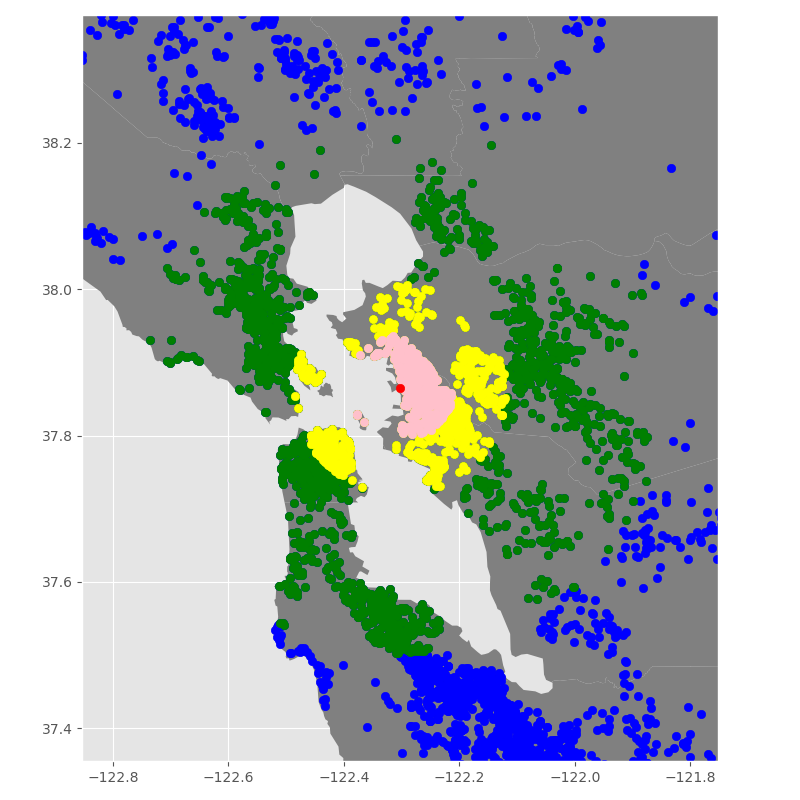
\includegraphics[width=0.8\textwidth]{appendix/site_plots/county-001_site-0013_epa-pa-concentric-ranges.png}
\caption{Map of EPA NAAQS-primary monitoring station (red) surrounded by PurpleAir monitors within 5-mile (pink), 10-mile (yellow), and 25-mile (green) radii.This preliminary analysis uses the PurpleAir sensors within 5 miles (pink markers). This monitor is at site 0013 in county 001 (FIPS code).}
\label{fig:concentric_purpleair_001-0013}
\end{figure}
\begin{figure}
\centering
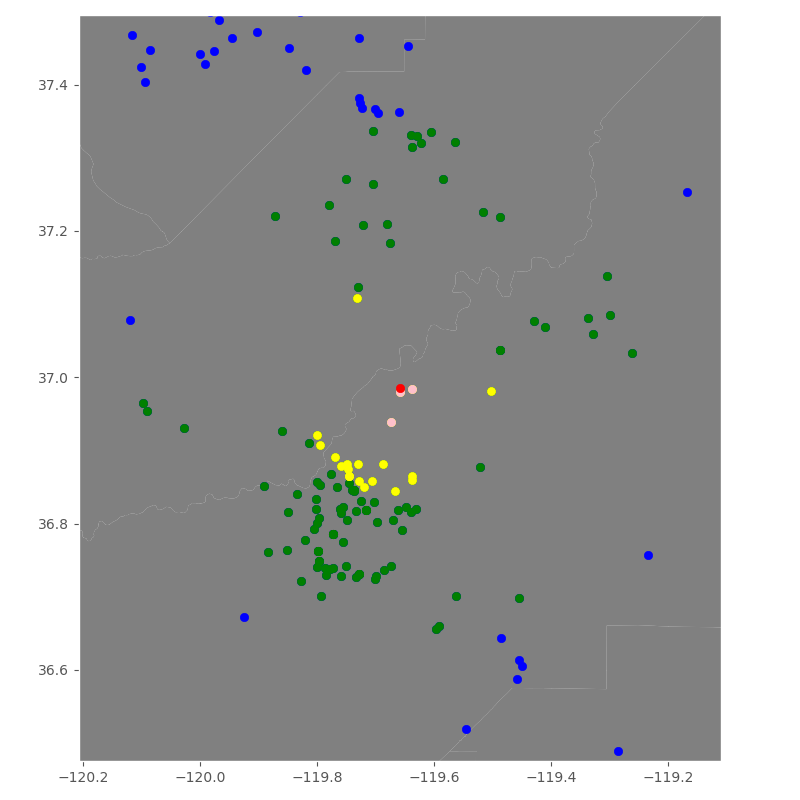
\includegraphics[width=0.8\textwidth]{appendix/site_plots/county-019_site-0500_epa-pa-concentric-ranges.png}
\caption{Map of EPA NAAQS-primary monitoring station (red) surrounded by PurpleAir monitors within 5-mile (pink), 10-mile (yellow), and 25-mile (green) radii.This preliminary analysis uses the PurpleAir sensors within 5 miles (pink markers). This monitor is at site 0500 in county 019 (FIPS code).}
\label{fig:concentric_purpleair_019-0500}
\end{figure}
\begin{figure}
\centering
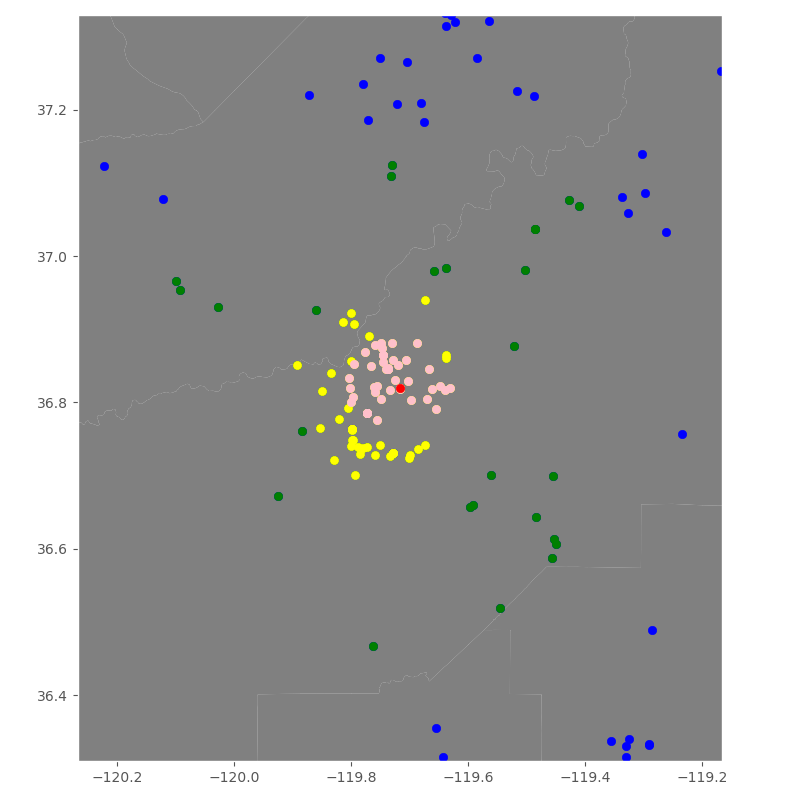
\includegraphics[width=0.8\textwidth]{appendix/site_plots/county-019_site-5001_epa-pa-concentric-ranges.png}
\caption{Map of EPA NAAQS-primary monitoring station (red) surrounded by PurpleAir monitors within 5-mile (pink), 10-mile (yellow), and 25-mile (green) radii.This preliminary analysis uses the PurpleAir sensors within 5 miles (pink markers). This monitor is at site 5001 in county 019 (FIPS code).}
\label{fig:concentric_purpleair_019-5001}
\end{figure}
\begin{figure}
\centering
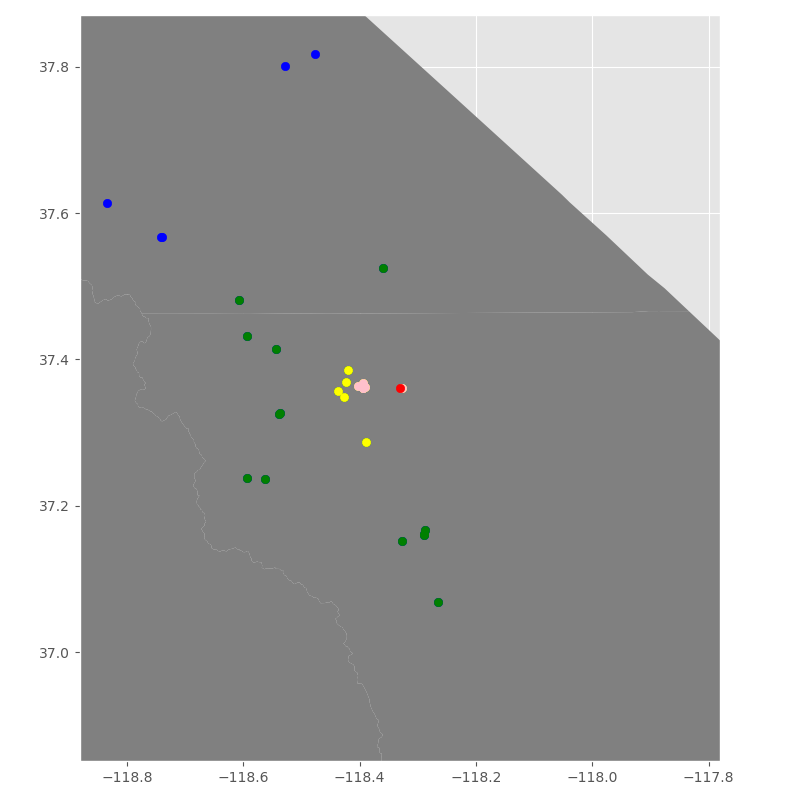
\includegraphics[width=0.8\textwidth]{appendix/site_plots/county-027_site-0002_epa-pa-concentric-ranges.png}
\caption{Map of EPA NAAQS-primary monitoring station (red) surrounded by PurpleAir monitors within 5-mile (pink), 10-mile (yellow), and 25-mile (green) radii.This preliminary analysis uses the PurpleAir sensors within 5 miles (pink markers). This monitor is at site 0002 in county 027 (FIPS code).}
\label{fig:concentric_purpleair_027-0002}
\end{figure}
\begin{figure}
\centering
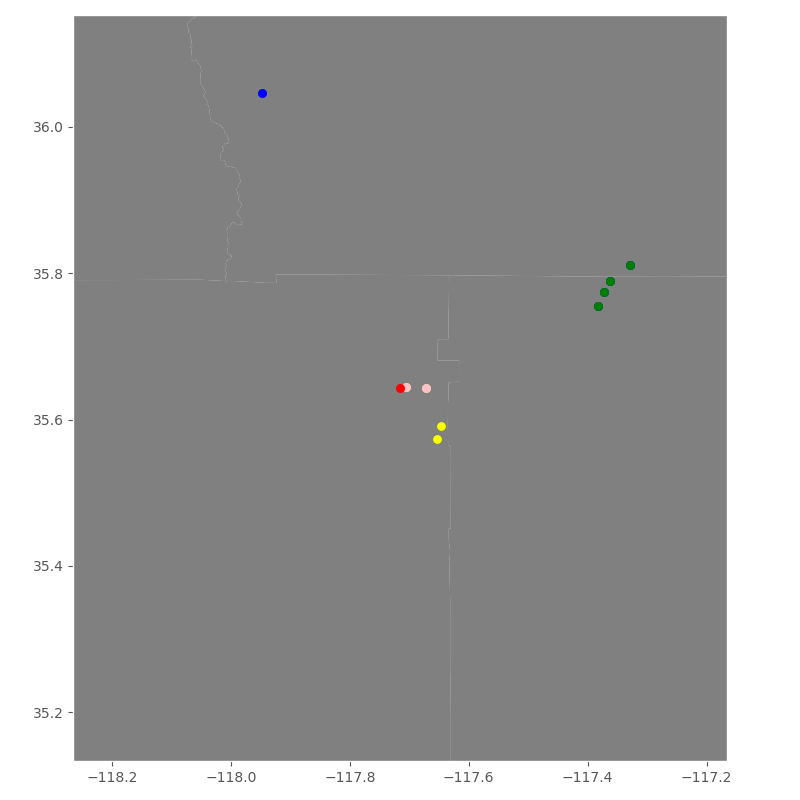
\includegraphics[width=0.8\textwidth]{appendix/site_plots/county-029_site-0018_epa-pa-concentric-ranges.png}
\caption{Map of EPA NAAQS-primary monitoring station (red) surrounded by PurpleAir monitors within 5-mile (pink), 10-mile (yellow), and 25-mile (green) radii.This preliminary analysis uses the PurpleAir sensors within 5 miles (pink markers). This monitor is at site 0018 in county 029 (FIPS code).}
\label{fig:concentric_purpleair_029-0018}
\end{figure}
\begin{figure}
\centering
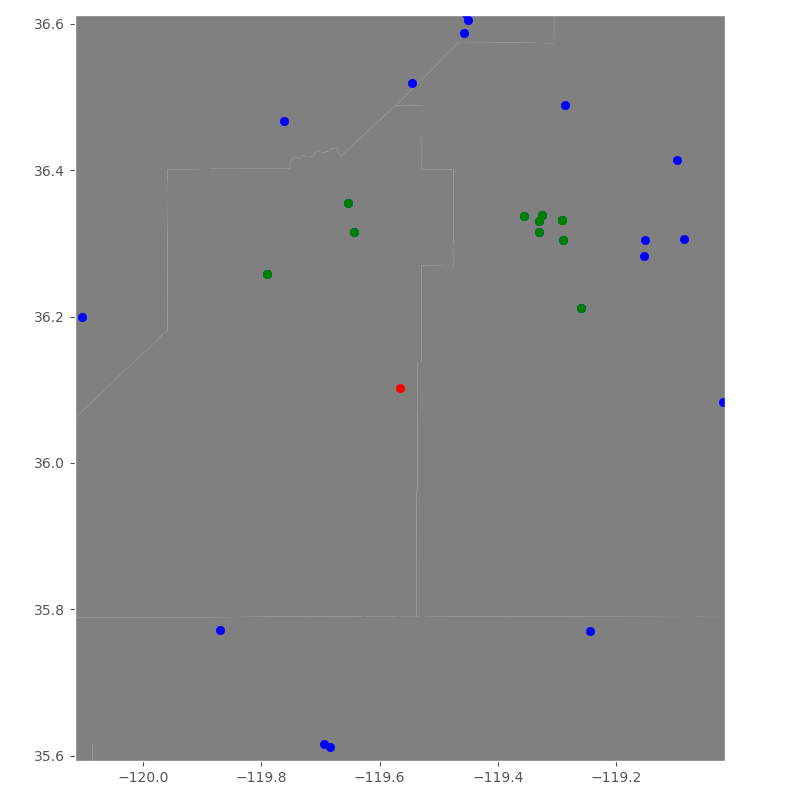
\includegraphics[width=0.8\textwidth]{appendix/site_plots/county-031_site-0004_epa-pa-concentric-ranges.png}
\caption{Map of EPA NAAQS-primary monitoring station (red) surrounded by PurpleAir monitors within 5-mile (pink), 10-mile (yellow), and 25-mile (green) radii.This preliminary analysis uses the PurpleAir sensors within 5 miles (pink markers). This monitor is at site 0004 in county 031 (FIPS code).}
\label{fig:concentric_purpleair_031-0004}
\end{figure}
\begin{figure}
\centering
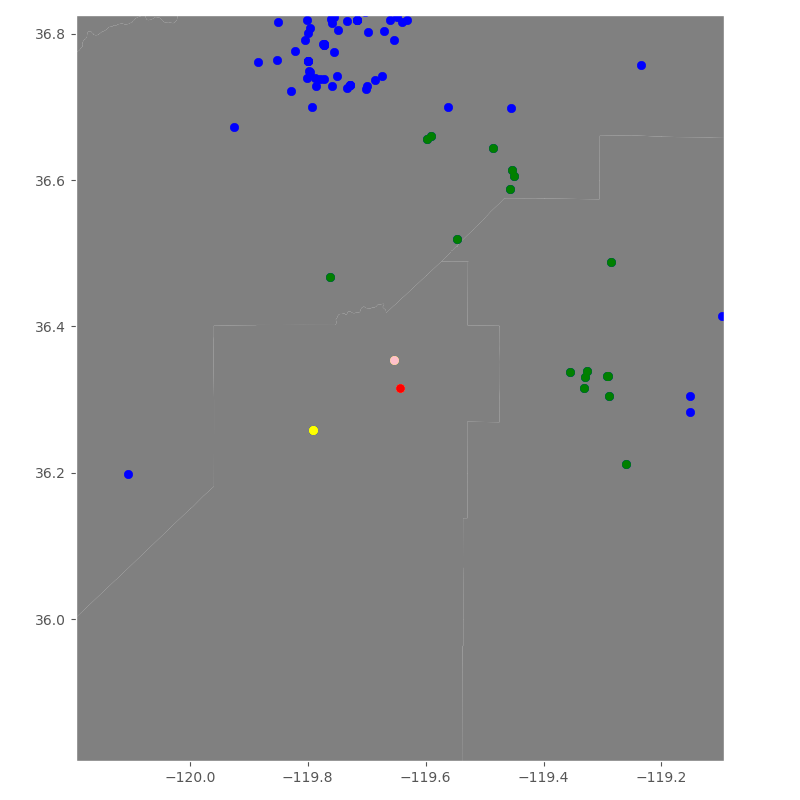
\includegraphics[width=0.8\textwidth]{appendix/site_plots/county-031_site-1004_epa-pa-concentric-ranges.png}
\caption{Map of EPA NAAQS-primary monitoring station (red) surrounded by PurpleAir monitors within 5-mile (pink), 10-mile (yellow), and 25-mile (green) radii.This preliminary analysis uses the PurpleAir sensors within 5 miles (pink markers). This monitor is at site 1004 in county 031 (FIPS code).}
\label{fig:concentric_purpleair_031-1004}
\end{figure}
\begin{figure}
\centering
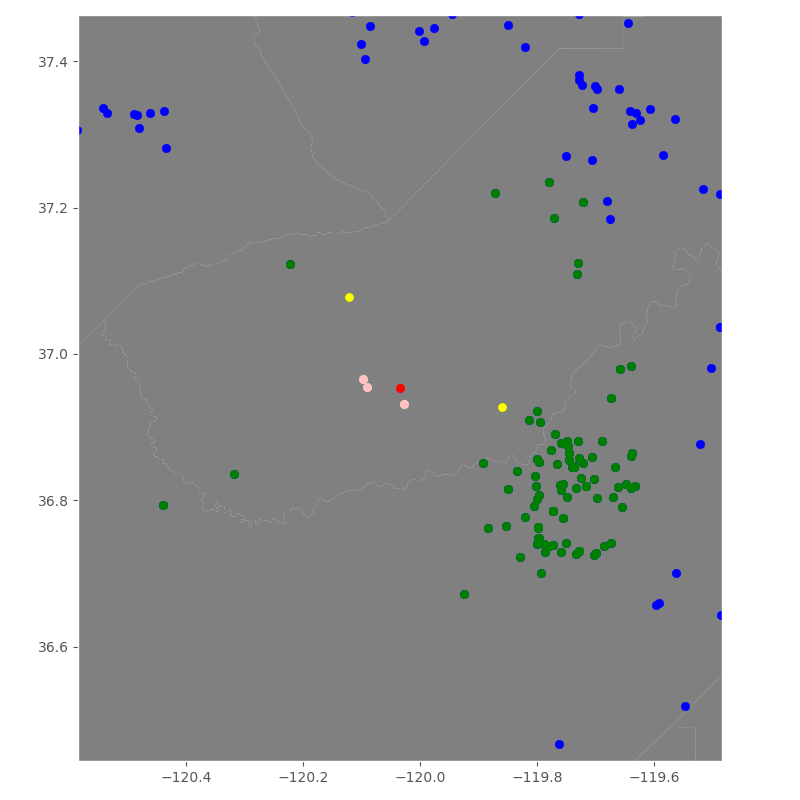
\includegraphics[width=0.8\textwidth]{appendix/site_plots/county-039_site-2010_epa-pa-concentric-ranges.png}
\caption{Map of EPA NAAQS-primary monitoring station (red) surrounded by PurpleAir monitors within 5-mile (pink), 10-mile (yellow), and 25-mile (green) radii.This preliminary analysis uses the PurpleAir sensors within 5 miles (pink markers). This monitor is at site 2010 in county 039 (FIPS code).}
\label{fig:concentric_purpleair_039-2010}
\end{figure}
\begin{figure}
\centering
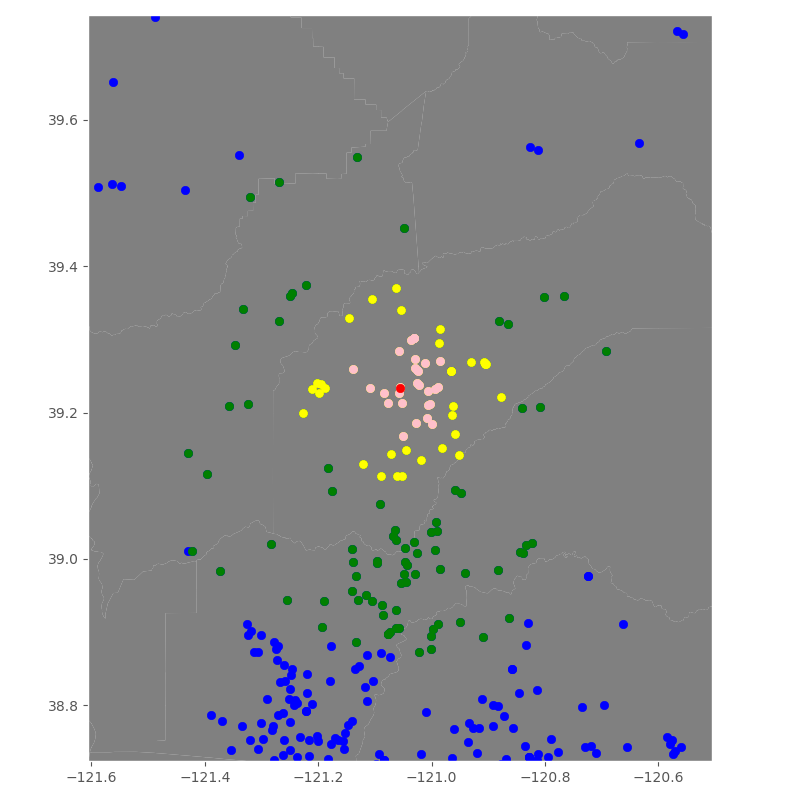
\includegraphics[width=0.8\textwidth]{appendix/site_plots/county-057_site-0005_epa-pa-concentric-ranges.png}
\caption{Map of EPA NAAQS-primary monitoring station (red) surrounded by PurpleAir monitors within 5-mile (pink), 10-mile (yellow), and 25-mile (green) radii.This preliminary analysis uses the PurpleAir sensors within 5 miles (pink markers). This monitor is at site 0005 in county 057 (FIPS code).}
\label{fig:concentric_purpleair_057-0005}
\end{figure}
\begin{figure}
\centering
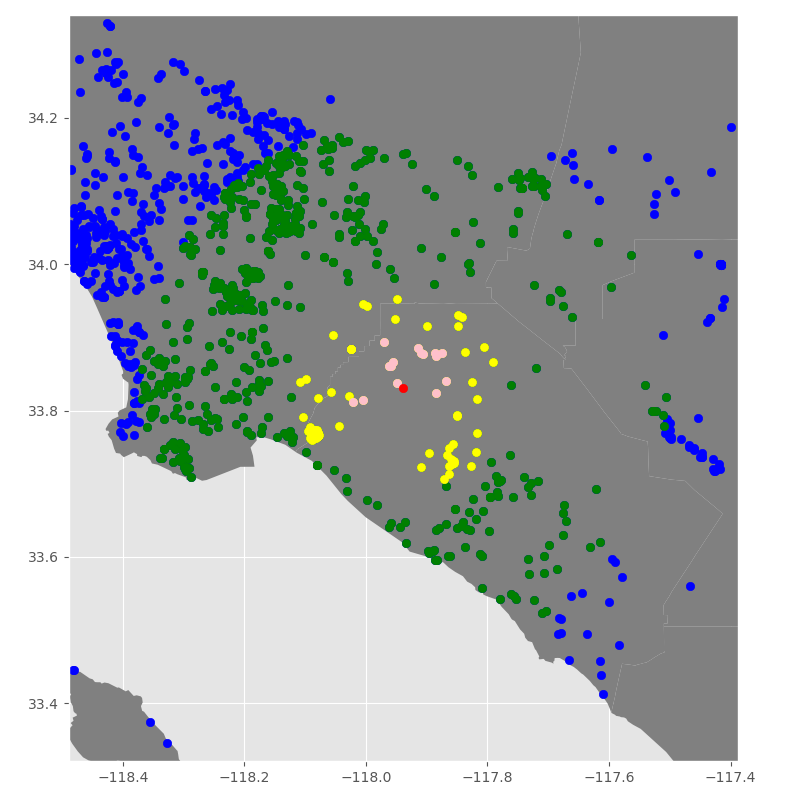
\includegraphics[width=0.8\textwidth]{appendix/site_plots/county-059_site-0007_epa-pa-concentric-ranges.png}
\caption{Map of EPA NAAQS-primary monitoring station (red) surrounded by PurpleAir monitors within 5-mile (pink), 10-mile (yellow), and 25-mile (green) radii.This preliminary analysis uses the PurpleAir sensors within 5 miles (pink markers). This monitor is at site 0007 in county 059 (FIPS code).}
\label{fig:concentric_purpleair_059-0007}
\end{figure}
\begin{figure}
\centering
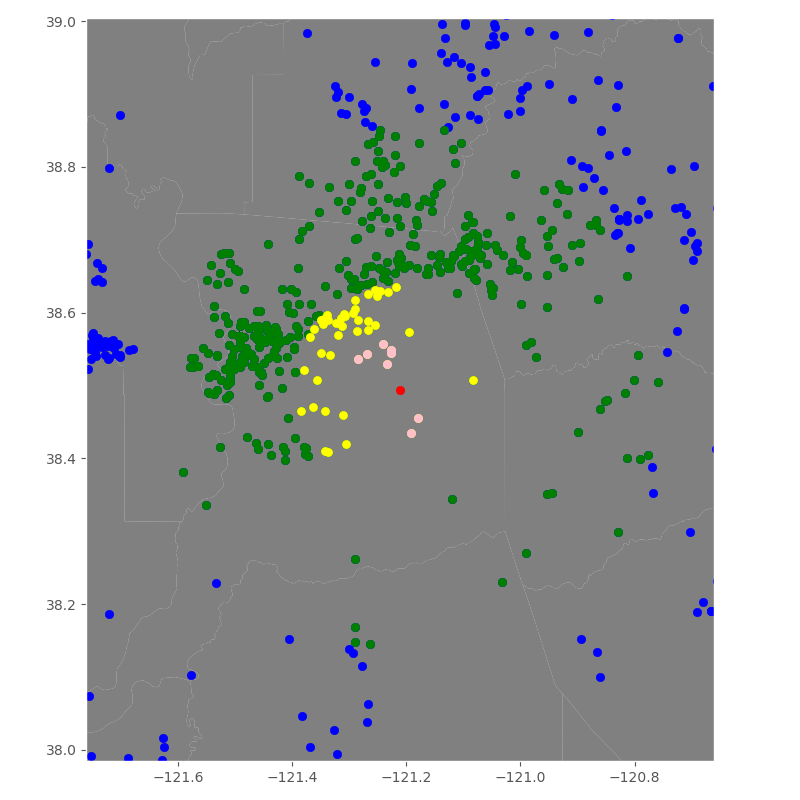
\includegraphics[width=0.8\textwidth]{appendix/site_plots/county-067_site-5003_epa-pa-concentric-ranges.png}
\caption{Map of EPA NAAQS-primary monitoring station (red) surrounded by PurpleAir monitors within 5-mile (pink), 10-mile (yellow), and 25-mile (green) radii.This preliminary analysis uses the PurpleAir sensors within 5 miles (pink markers). This monitor is at site 5003 in county 067 (FIPS code).}
\label{fig:concentric_purpleair_067-5003}
\end{figure}
\begin{figure}
\centering
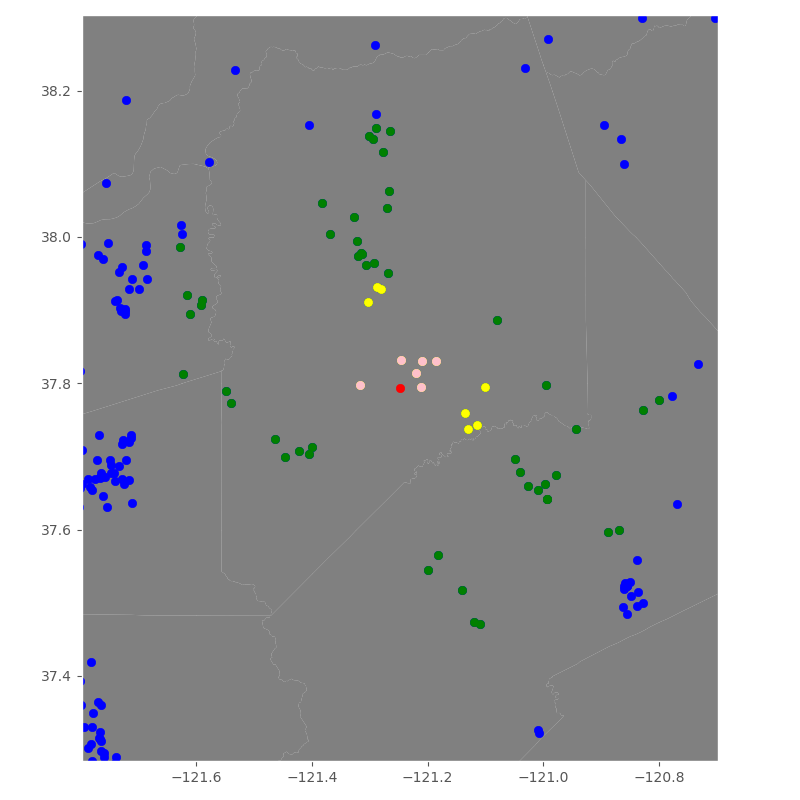
\includegraphics[width=0.8\textwidth]{appendix/site_plots/county-077_site-2010_epa-pa-concentric-ranges.png}
\caption{Map of EPA NAAQS-primary monitoring station (red) surrounded by PurpleAir monitors within 5-mile (pink), 10-mile (yellow), and 25-mile (green) radii.This preliminary analysis uses the PurpleAir sensors within 5 miles (pink markers). This monitor is at site 2010 in county 077 (FIPS code).}
\label{fig:concentric_purpleair_077-2010}
\end{figure}
\begin{figure}
\centering
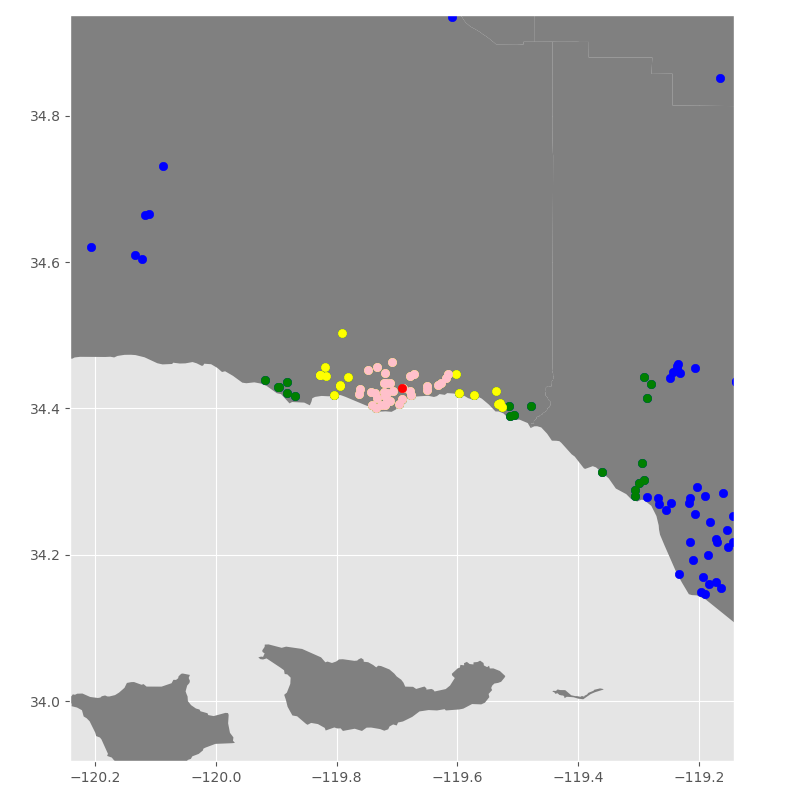
\includegraphics[width=0.8\textwidth]{appendix/site_plots/county-083_site-0011_epa-pa-concentric-ranges.png}
\caption{Map of EPA NAAQS-primary monitoring station (red) surrounded by PurpleAir monitors within 5-mile (pink), 10-mile (yellow), and 25-mile (green) radii.This preliminary analysis uses the PurpleAir sensors within 5 miles (pink markers). This monitor is at site 0011 in county 083 (FIPS code).}
\label{fig:concentric_purpleair_083-0011}
\end{figure}
\begin{figure}
\centering
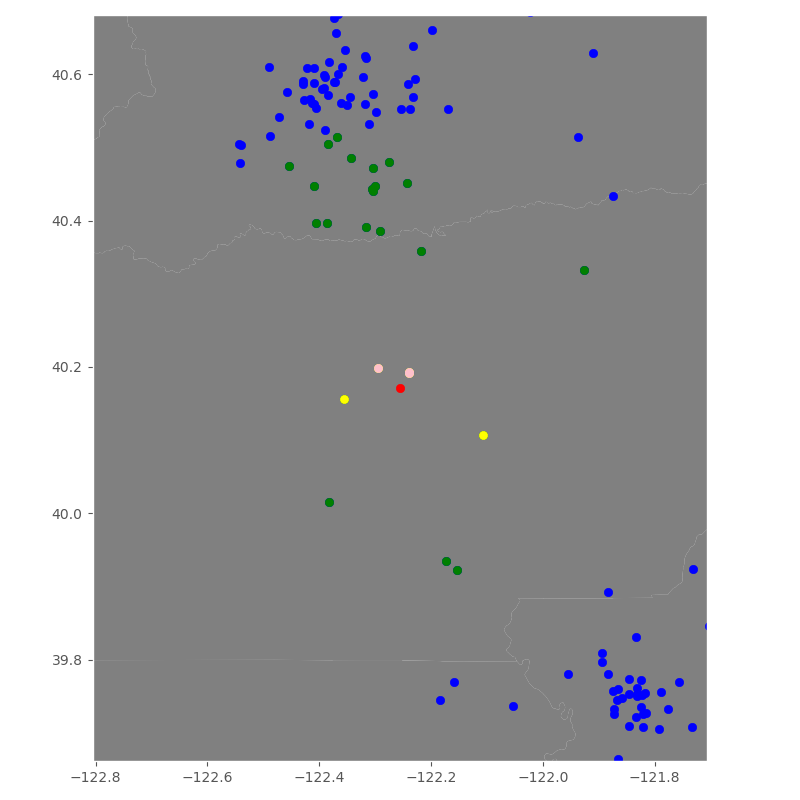
\includegraphics[width=0.8\textwidth]{appendix/site_plots/county-103_site-0007_epa-pa-concentric-ranges.png}
\caption{Map of EPA NAAQS-primary monitoring station (red) surrounded by PurpleAir monitors within 5-mile (pink), 10-mile (yellow), and 25-mile (green) radii.This preliminary analysis uses the PurpleAir sensors within 5 miles (pink markers). This monitor is at site 0007 in county 103 (FIPS code).}
\label{fig:concentric_purpleair_103-0007}
\end{figure}
%=========================================
%  PurpleAir Hourly Observation Coverage
%=========================================
\begin{figure}
\centering
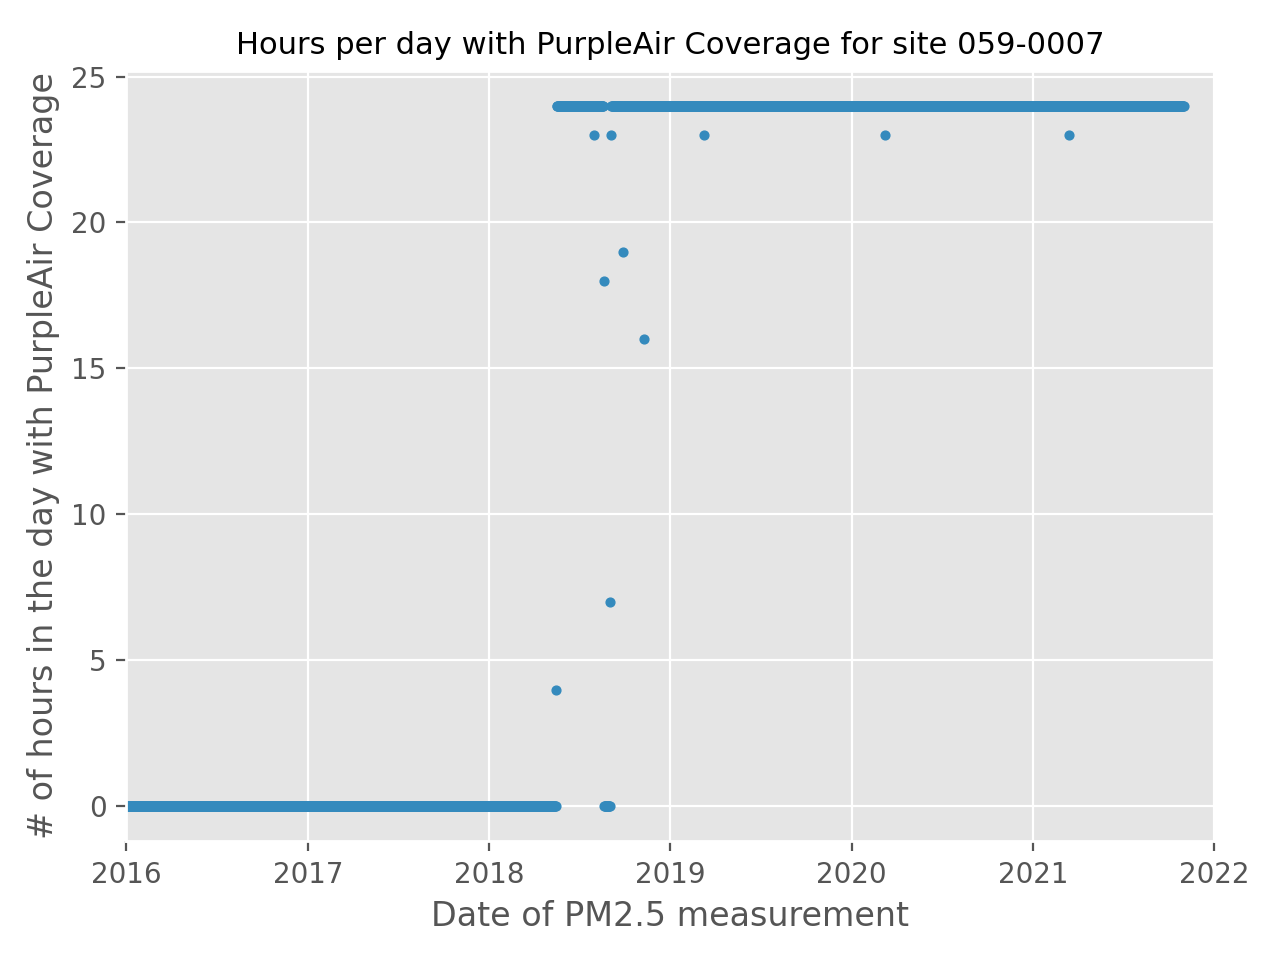
\includegraphics[width=0.8\textwidth]{appendix/site_plots/site-059-0007_pa-daily-covereage.png}
\caption{Scatter plot indicating the number of hours in each day that this NAAQS monitor has PurpleAir coverage. An hour has PurpleAir coverage if there are any PurpleAir sensor readings within the 5-mile radius of the monitor site for that hour. The weighted average is calculated for that hour using all the available PurpleAir readings within 5 miles. This monitor is at site 0007 in county 059 (FIPS code).}
\label{fig:hourly_coverage_059-0007}
\end{figure}
\begin{figure}
\centering
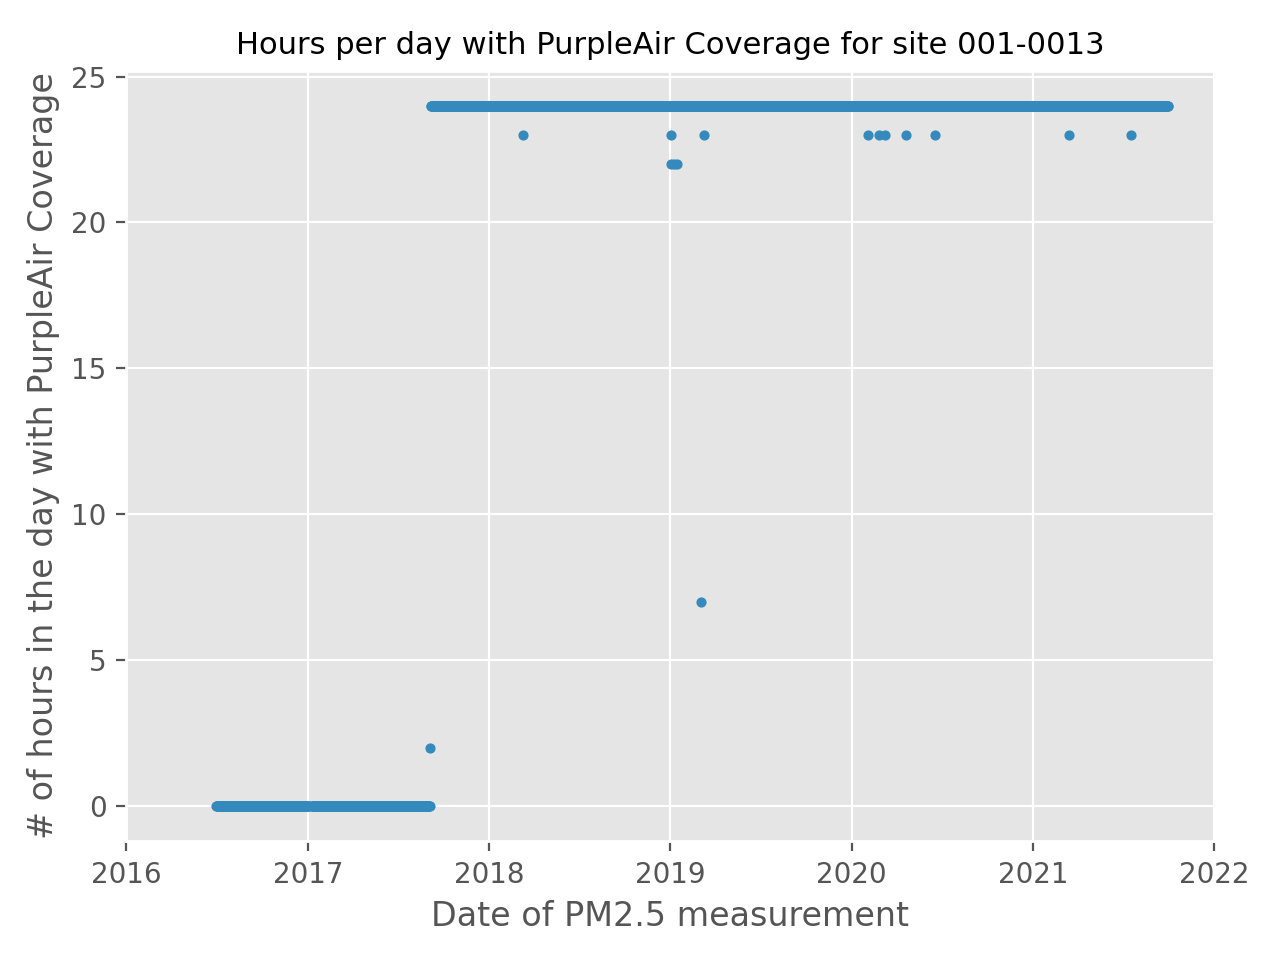
\includegraphics[width=0.8\textwidth]{appendix/site_plots/site-001-0013_pa-daily-covereage.png}
\caption{Scatter plot indicating the number of hours in each day that this NAAQS monitor has PurpleAir coverage. An hour has PurpleAir coverage if there are any PurpleAir sensor readings within the 5-mile radius of the monitor site for that hour. The weighted average is calculated for that hour using all the available PurpleAir readings within 5 miles. This monitor is at site 0013 in county 001 (FIPS code).}
\label{fig:hourly_coverage_001-0013}
\end{figure}
\begin{figure}
\centering
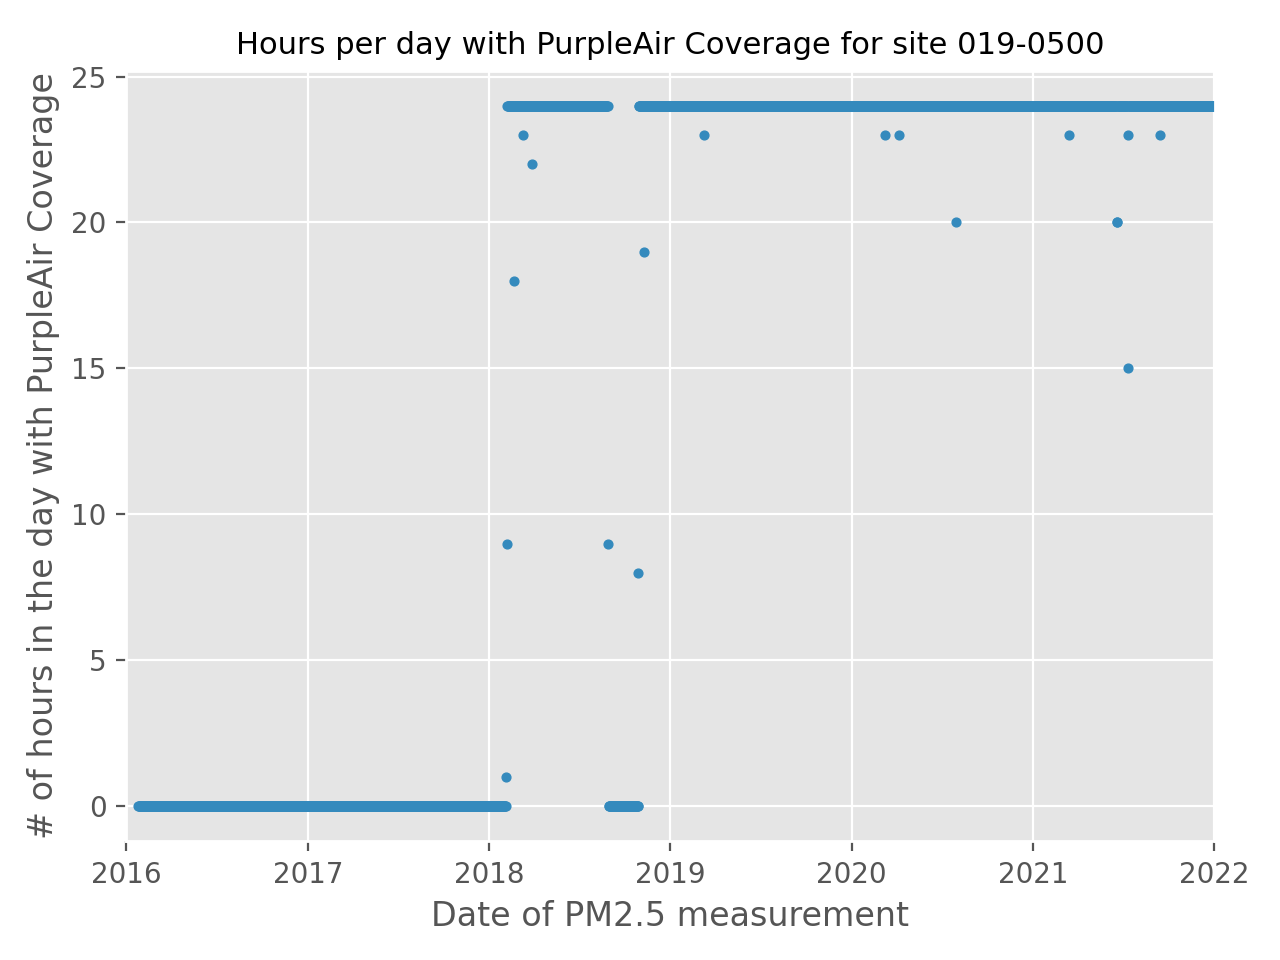
\includegraphics[width=0.8\textwidth]{appendix/site_plots/site-019-0500_pa-daily-covereage.png}
\caption{Scatter plot indicating the number of hours in each day that this NAAQS monitor has PurpleAir coverage. An hour has PurpleAir coverage if there are any PurpleAir sensor readings within the 5-mile radius of the monitor site for that hour. The weighted average is calculated for that hour using all the available PurpleAir readings within 5 miles. This monitor is at site 0500 in county 019 (FIPS code).}
\label{fig:hourly_coverage_019-0500}
\end{figure}
\begin{figure}
\centering
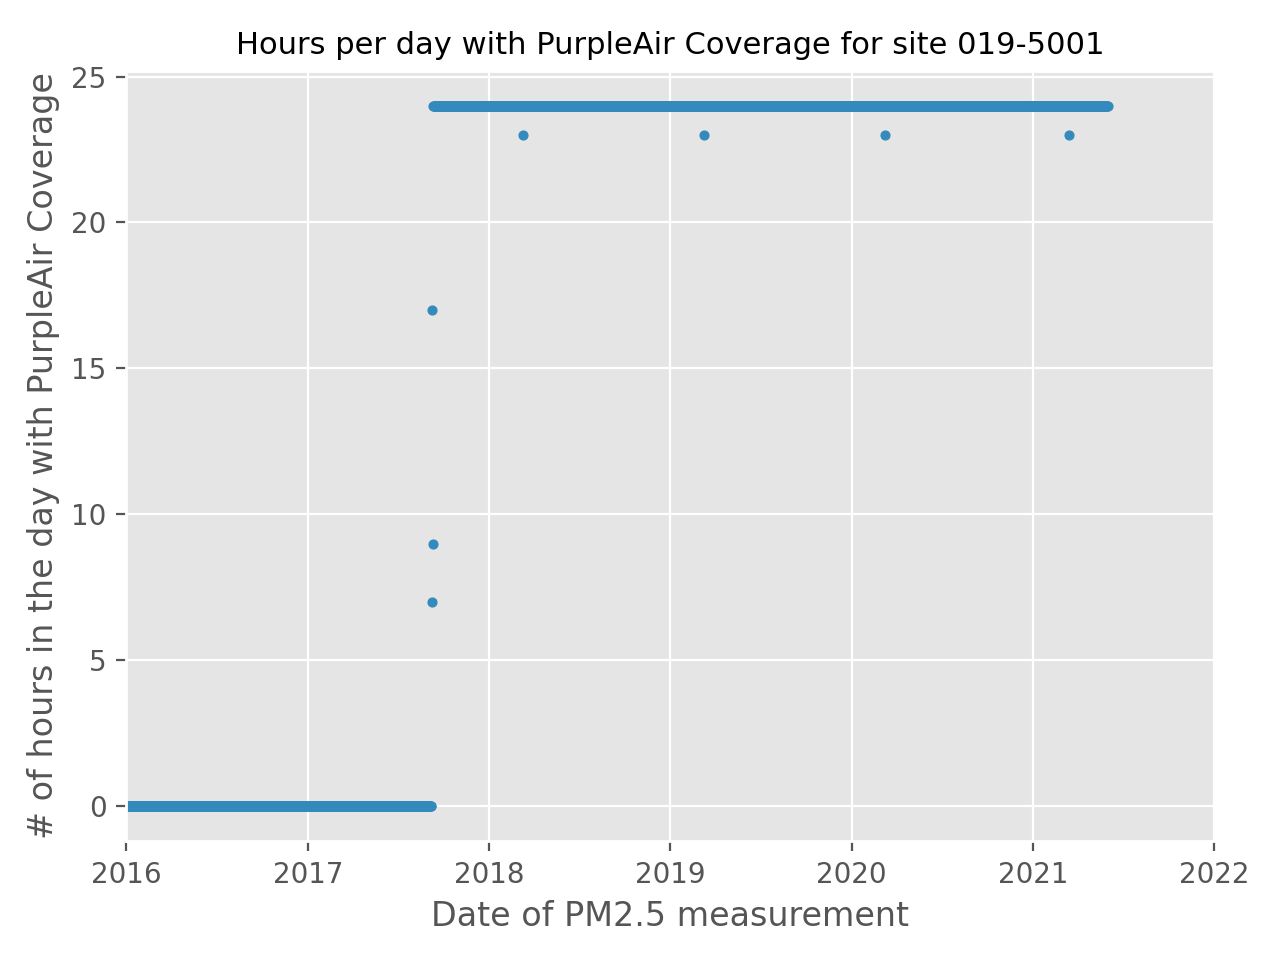
\includegraphics[width=0.8\textwidth]{appendix/site_plots/site-019-5001_pa-daily-covereage.png}
\caption{Scatter plot indicating the number of hours in each day that this NAAQS monitor has PurpleAir coverage. An hour has PurpleAir coverage if there are any PurpleAir sensor readings within the 5-mile radius of the monitor site for that hour. The weighted average is calculated for that hour using all the available PurpleAir readings within 5 miles. This monitor is at site 5001 in county 019 (FIPS code).}
\label{fig:hourly_coverage_019-5001}
\end{figure}
\begin{figure}
\centering
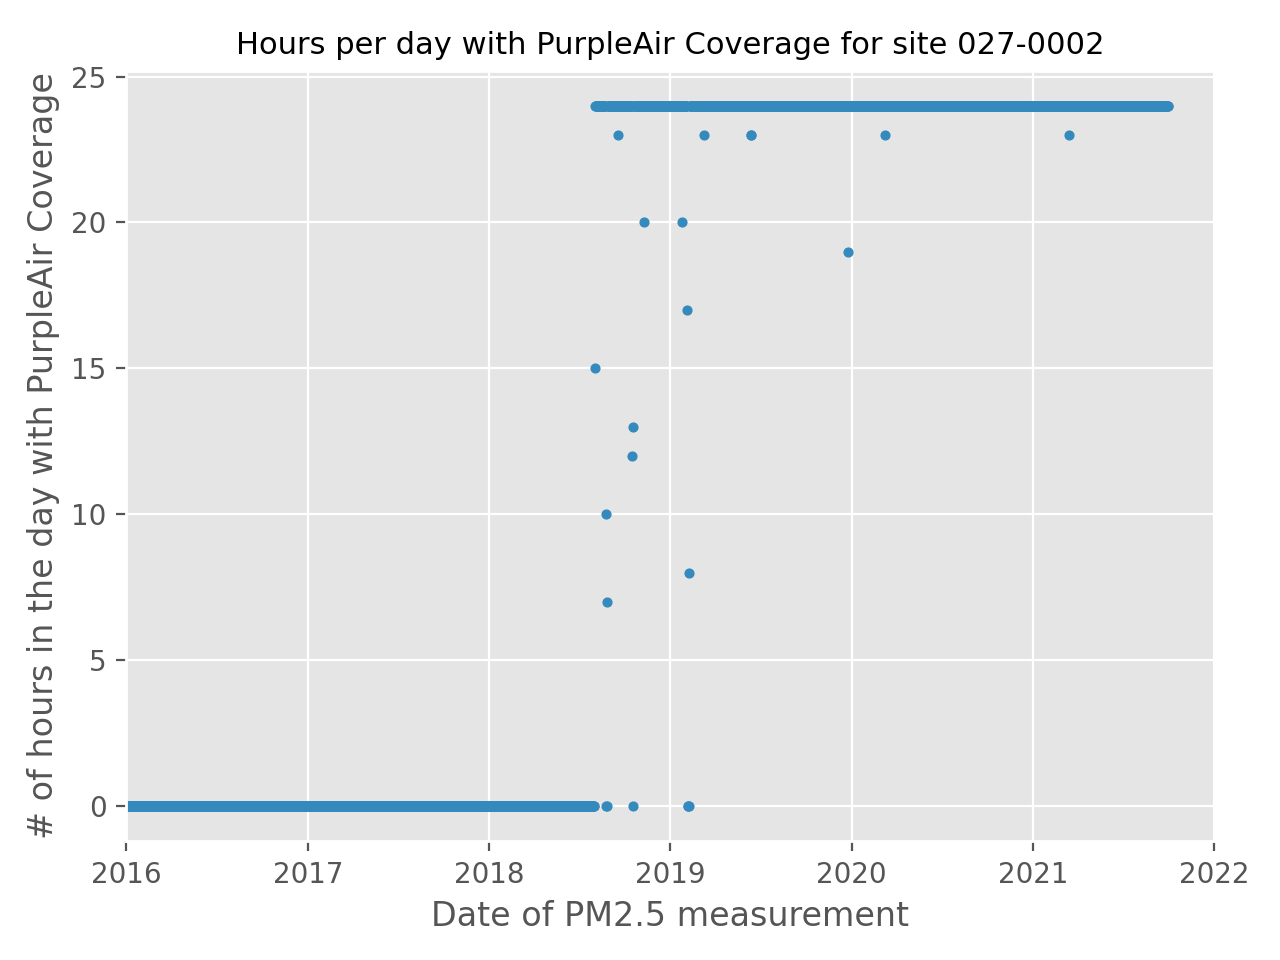
\includegraphics[width=0.8\textwidth]{appendix/site_plots/site-027-0002_pa-daily-covereage.png}
\caption{Scatter plot indicating the number of hours in each day that this NAAQS monitor has PurpleAir coverage. An hour has PurpleAir coverage if there are any PurpleAir sensor readings within the 5-mile radius of the monitor site for that hour. The weighted average is calculated for that hour using all the available PurpleAir readings within 5 miles. This monitor is at site 0002 in county 027 (FIPS code).}
\label{fig:hourly_coverage_027-0002}
\end{figure}
\begin{figure}
\centering
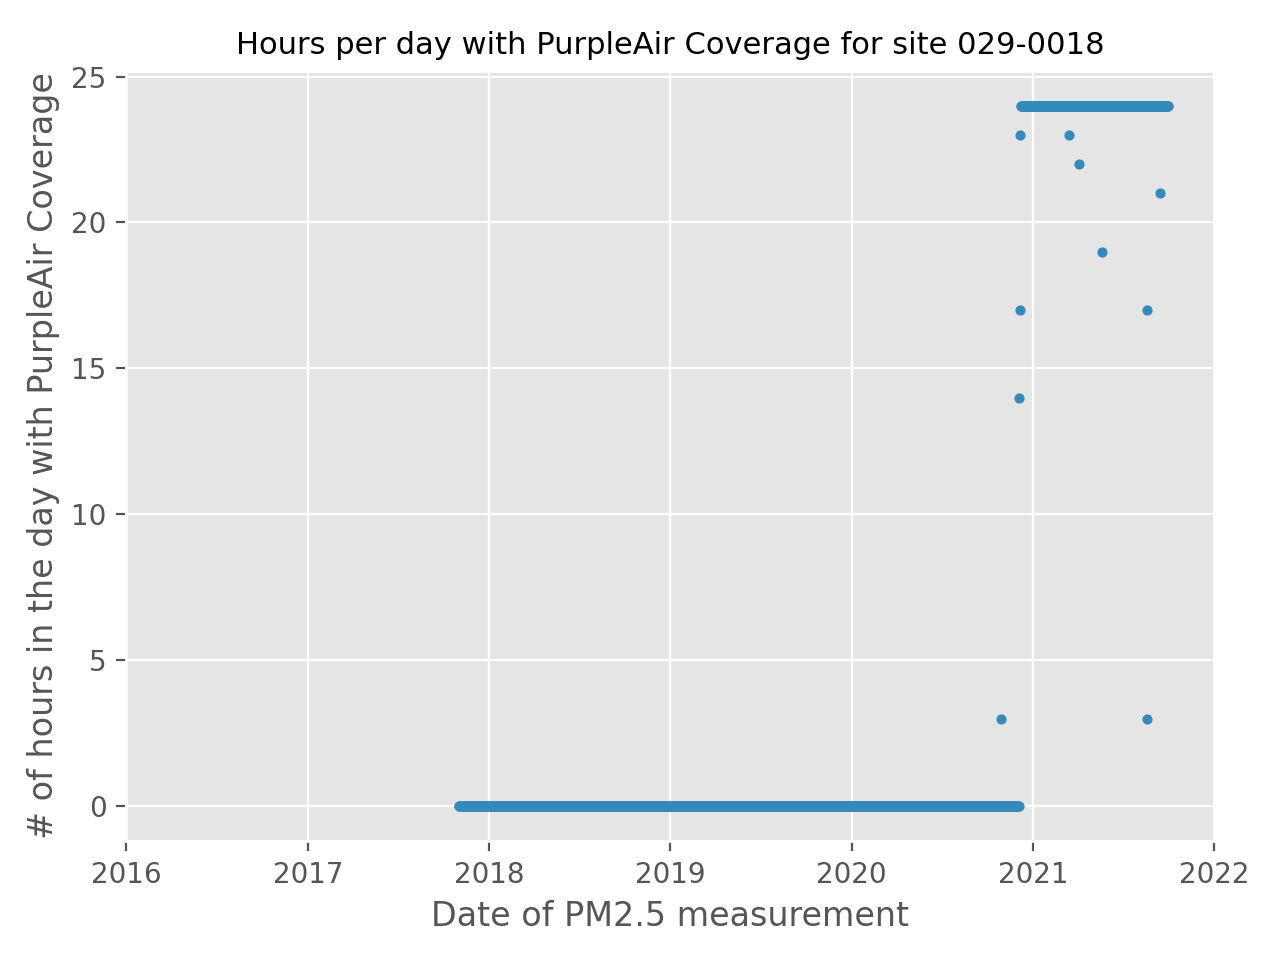
\includegraphics[width=0.8\textwidth]{appendix/site_plots/site-029-0018_pa-daily-covereage.png}
\caption{Scatter plot indicating the number of hours in each day that this NAAQS monitor has PurpleAir coverage. An hour has PurpleAir coverage if there are any PurpleAir sensor readings within the 5-mile radius of the monitor site for that hour. The weighted average is calculated for that hour using all the available PurpleAir readings within 5 miles. This monitor is at site 0018 in county 029 (FIPS code).}
\label{fig:hourly_coverage_029-0018}
\end{figure}
\begin{figure}
\centering
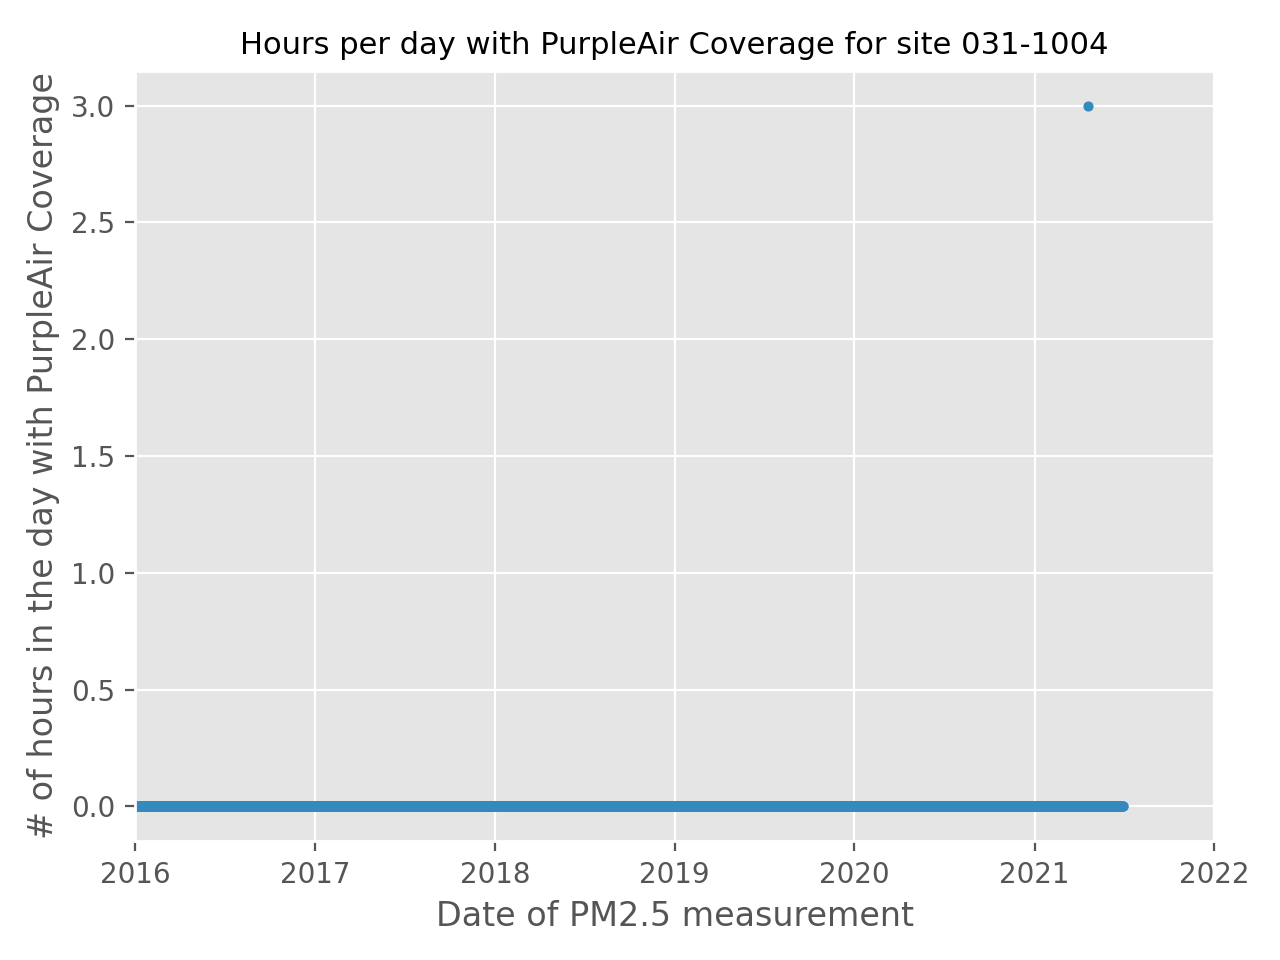
\includegraphics[width=0.8\textwidth]{appendix/site_plots/site-031-1004_pa-daily-covereage.png}
\caption{Scatter plot indicating the number of hours in each day that this NAAQS monitor has PurpleAir coverage. An hour has PurpleAir coverage if there are any PurpleAir sensor readings within the 5-mile radius of the monitor site for that hour. The weighted average is calculated for that hour using all the available PurpleAir readings within 5 miles. This monitor is at site 1004 in county 031 (FIPS code).}
\label{fig:hourly_coverage_031-1004}
\end{figure}
\begin{figure}
\centering
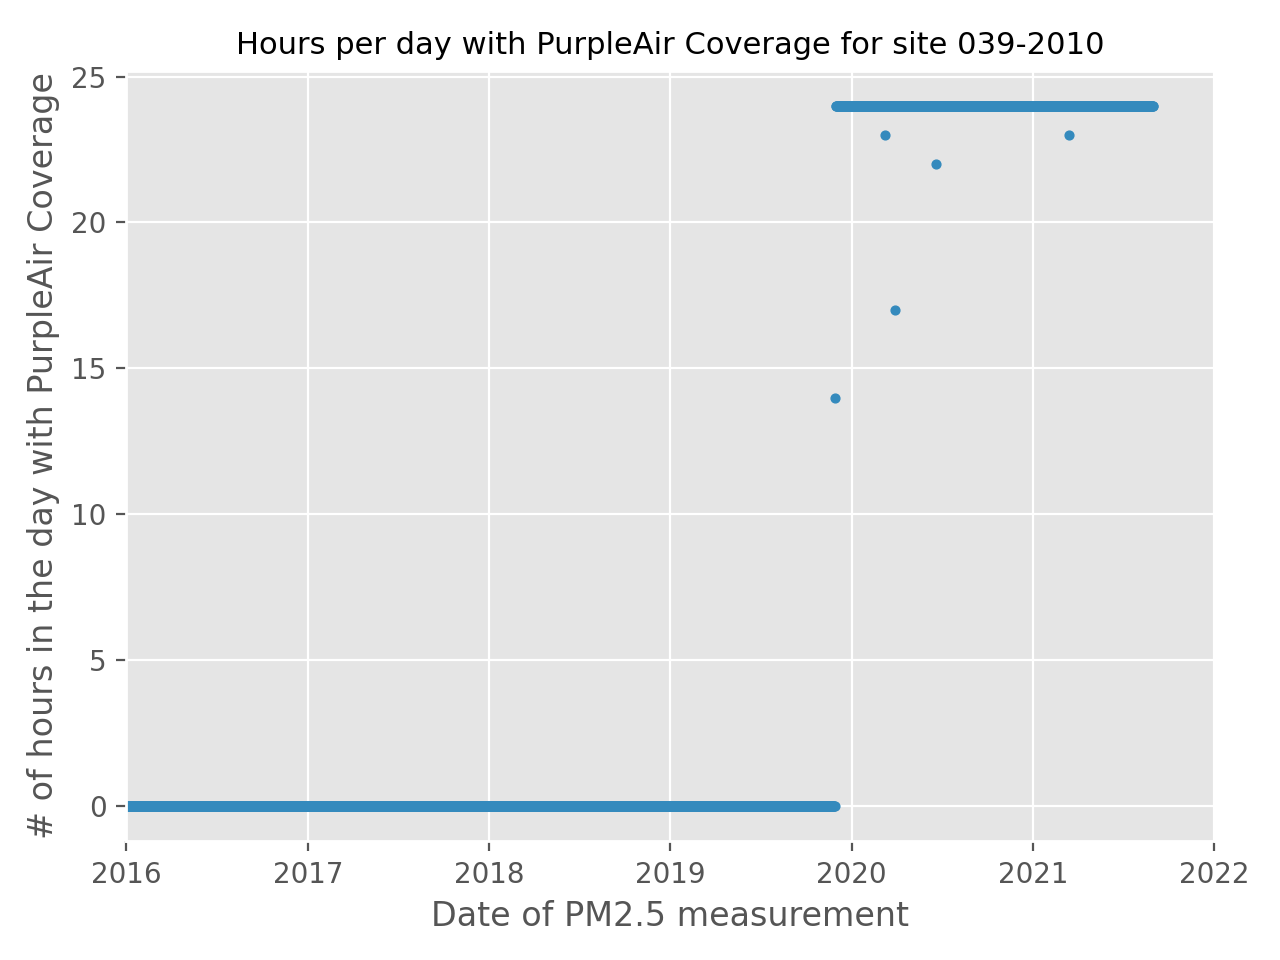
\includegraphics[width=0.8\textwidth]{appendix/site_plots/site-039-2010_pa-daily-covereage.png}
\caption{Scatter plot indicating the number of hours in each day that this NAAQS monitor has PurpleAir coverage. An hour has PurpleAir coverage if there are any PurpleAir sensor readings within the 5-mile radius of the monitor site for that hour. The weighted average is calculated for that hour using all the available PurpleAir readings within 5 miles. This monitor is at site 2010 in county 039 (FIPS code).}
\label{fig:hourly_coverage_039-2010}
\end{figure}
\begin{figure}
\centering
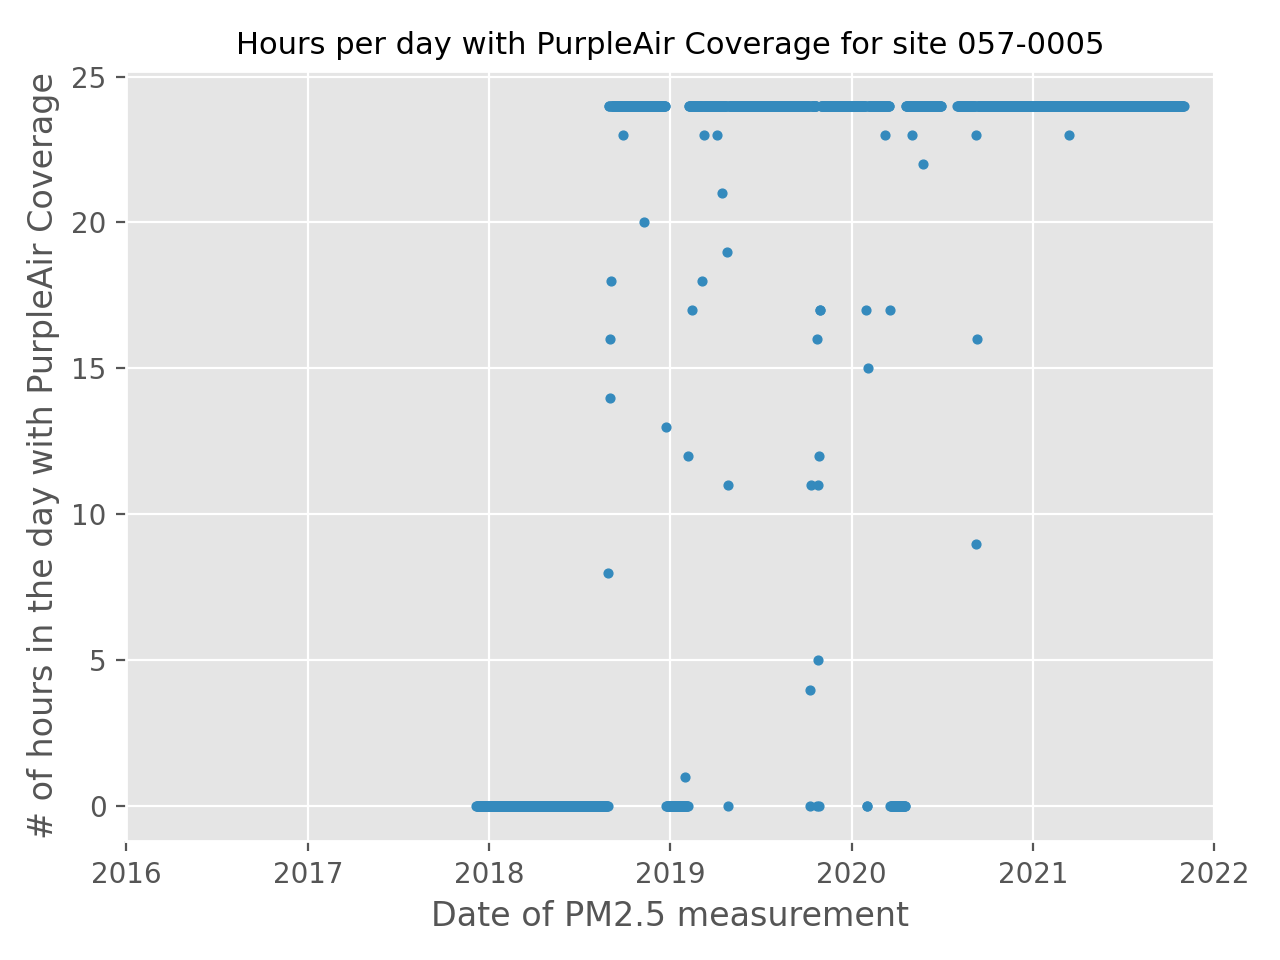
\includegraphics[width=0.8\textwidth]{appendix/site_plots/site-057-0005_pa-daily-covereage.png}
\caption{Scatter plot indicating the number of hours in each day that this NAAQS monitor has PurpleAir coverage. An hour has PurpleAir coverage if there are any PurpleAir sensor readings within the 5-mile radius of the monitor site for that hour. The weighted average is calculated for that hour using all the available PurpleAir readings within 5 miles. This monitor is at site 0005 in county 057 (FIPS code).}
\label{fig:hourly_coverage_057-0005}
\end{figure}
\begin{figure}
\centering
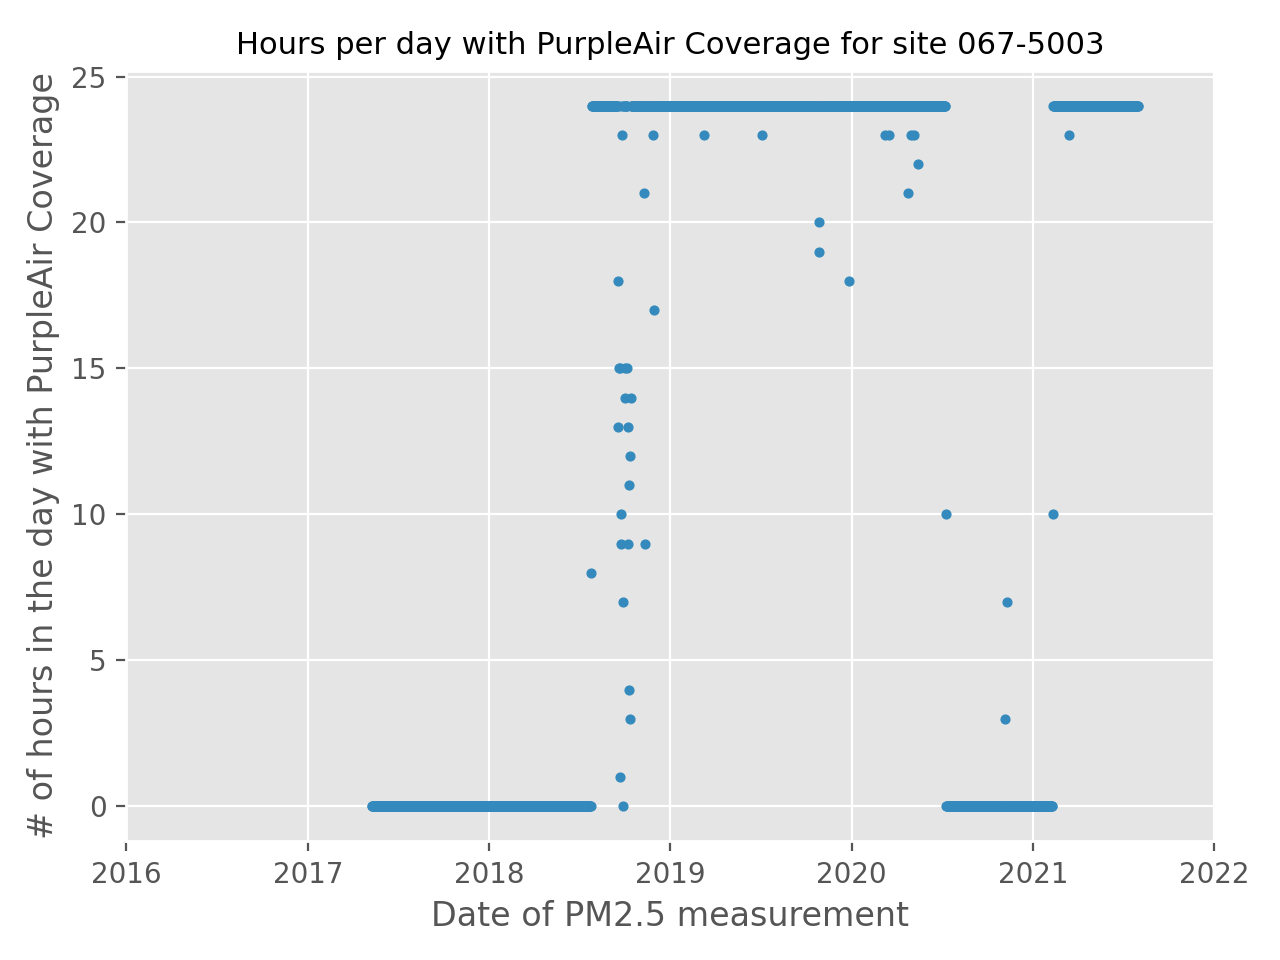
\includegraphics[width=0.8\textwidth]{appendix/site_plots/site-067-5003_pa-daily-covereage.png}
\caption{Scatter plot indicating the number of hours in each day that this NAAQS monitor has PurpleAir coverage. An hour has PurpleAir coverage if there are any PurpleAir sensor readings within the 5-mile radius of the monitor site for that hour. The weighted average is calculated for that hour using all the available PurpleAir readings within 5 miles. This monitor is at site 5003 in county 067 (FIPS code).}
\label{fig:hourly_coverage_067-5003}
\end{figure}
\begin{figure}
\centering
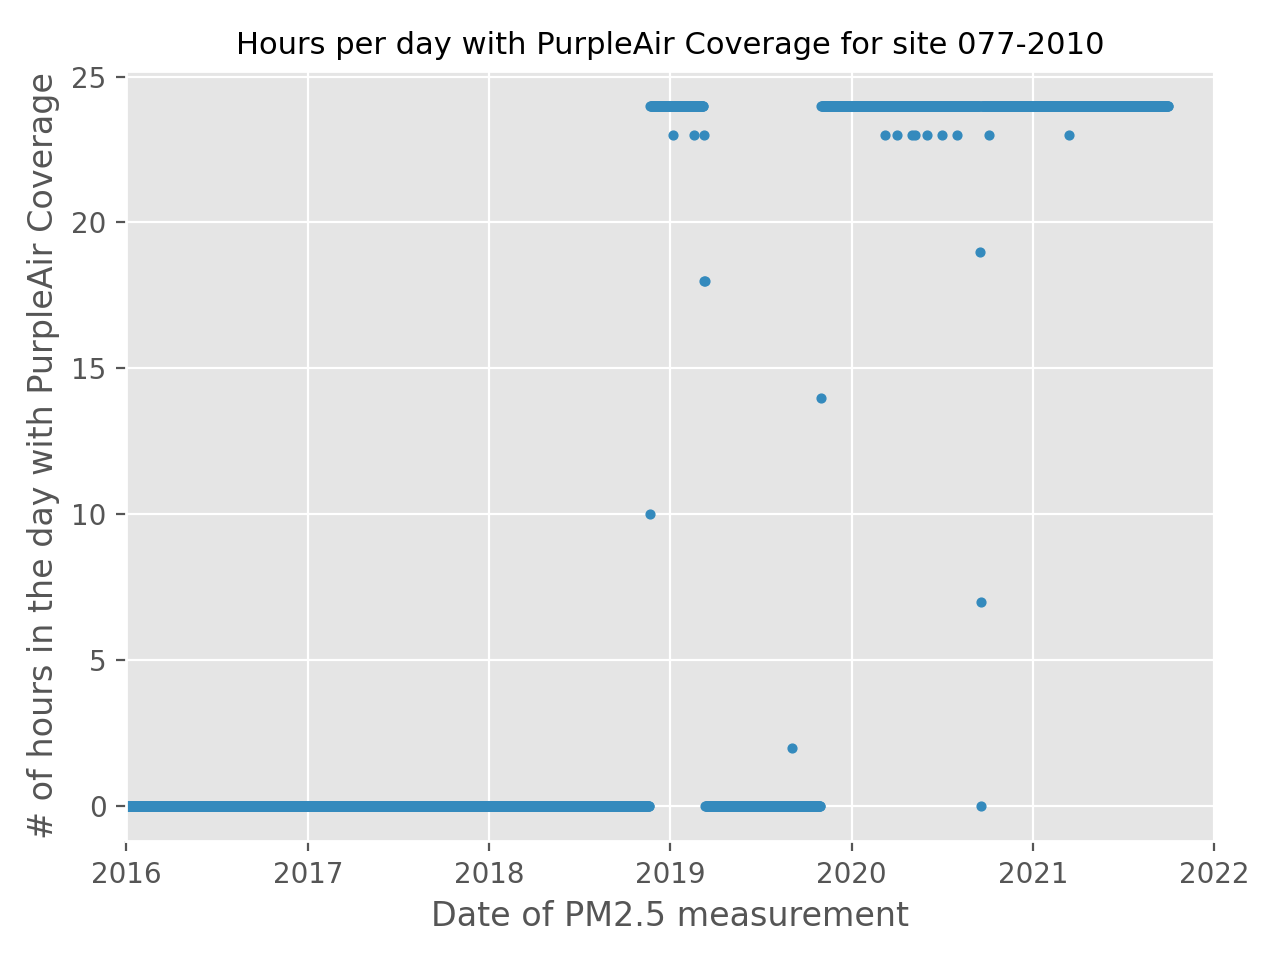
\includegraphics[width=0.8\textwidth]{appendix/site_plots/site-077-2010_pa-daily-covereage.png}
\caption{Scatter plot indicating the number of hours in each day that this NAAQS monitor has PurpleAir coverage. An hour has PurpleAir coverage if there are any PurpleAir sensor readings within the 5-mile radius of the monitor site for that hour. The weighted average is calculated for that hour using all the available PurpleAir readings within 5 miles. This monitor is at site 2010 in county 077 (FIPS code).}
\label{fig:hourly_coverage_077-2010}
\end{figure}
\begin{figure}
\centering
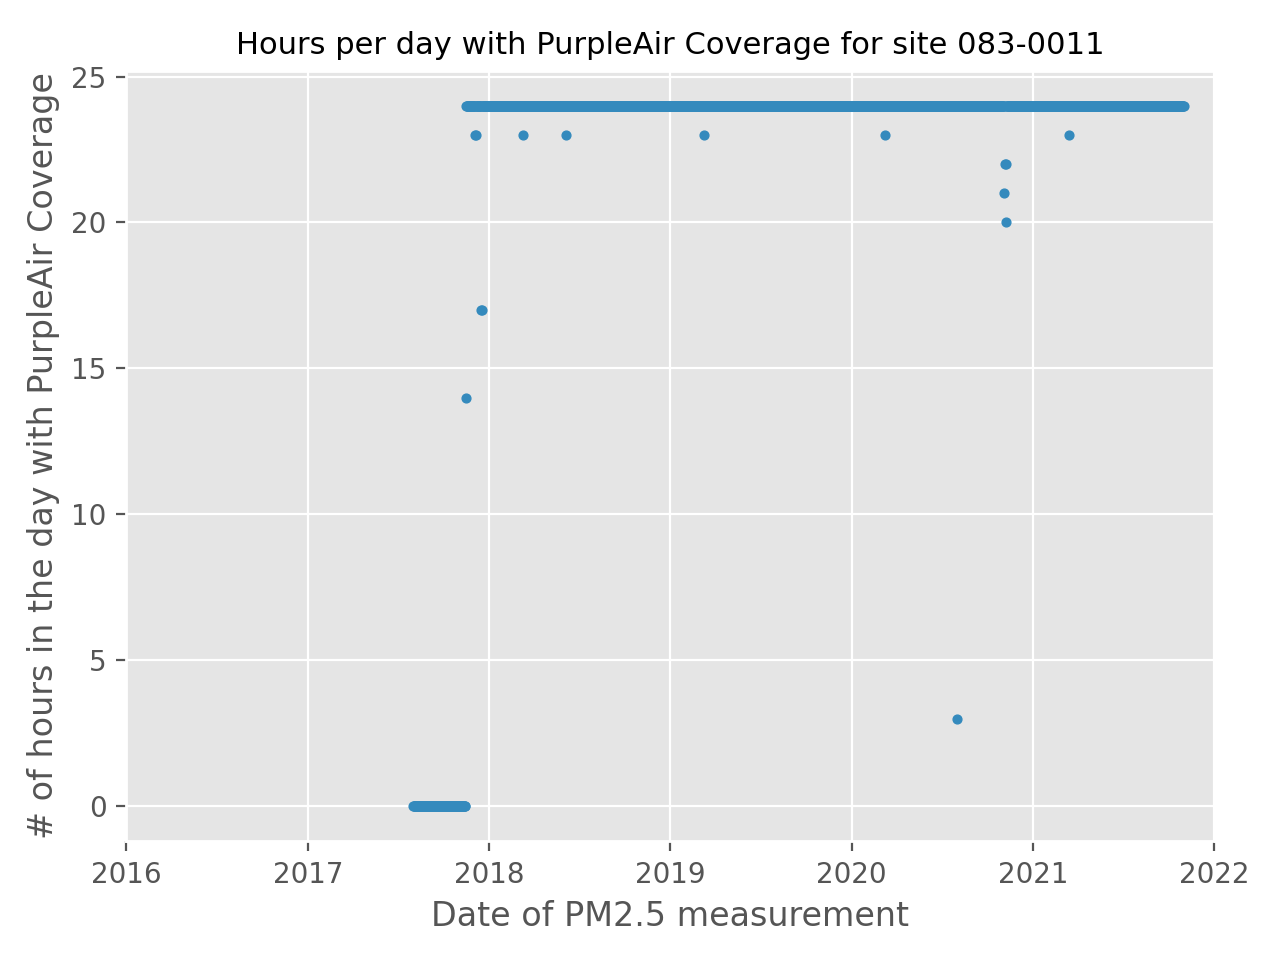
\includegraphics[width=0.8\textwidth]{appendix/site_plots/site-083-0011_pa-daily-covereage.png}
\caption{Scatter plot indicating the number of hours in each day that this NAAQS monitor has PurpleAir coverage. An hour has PurpleAir coverage if there are any PurpleAir sensor readings within the 5-mile radius of the monitor site for that hour. The weighted average is calculated for that hour using all the available PurpleAir readings within 5 miles. This monitor is at site 0011 in county 083 (FIPS code).}
\label{fig:hourly_coverage_083-0011}
\end{figure}
\begin{figure}
\centering
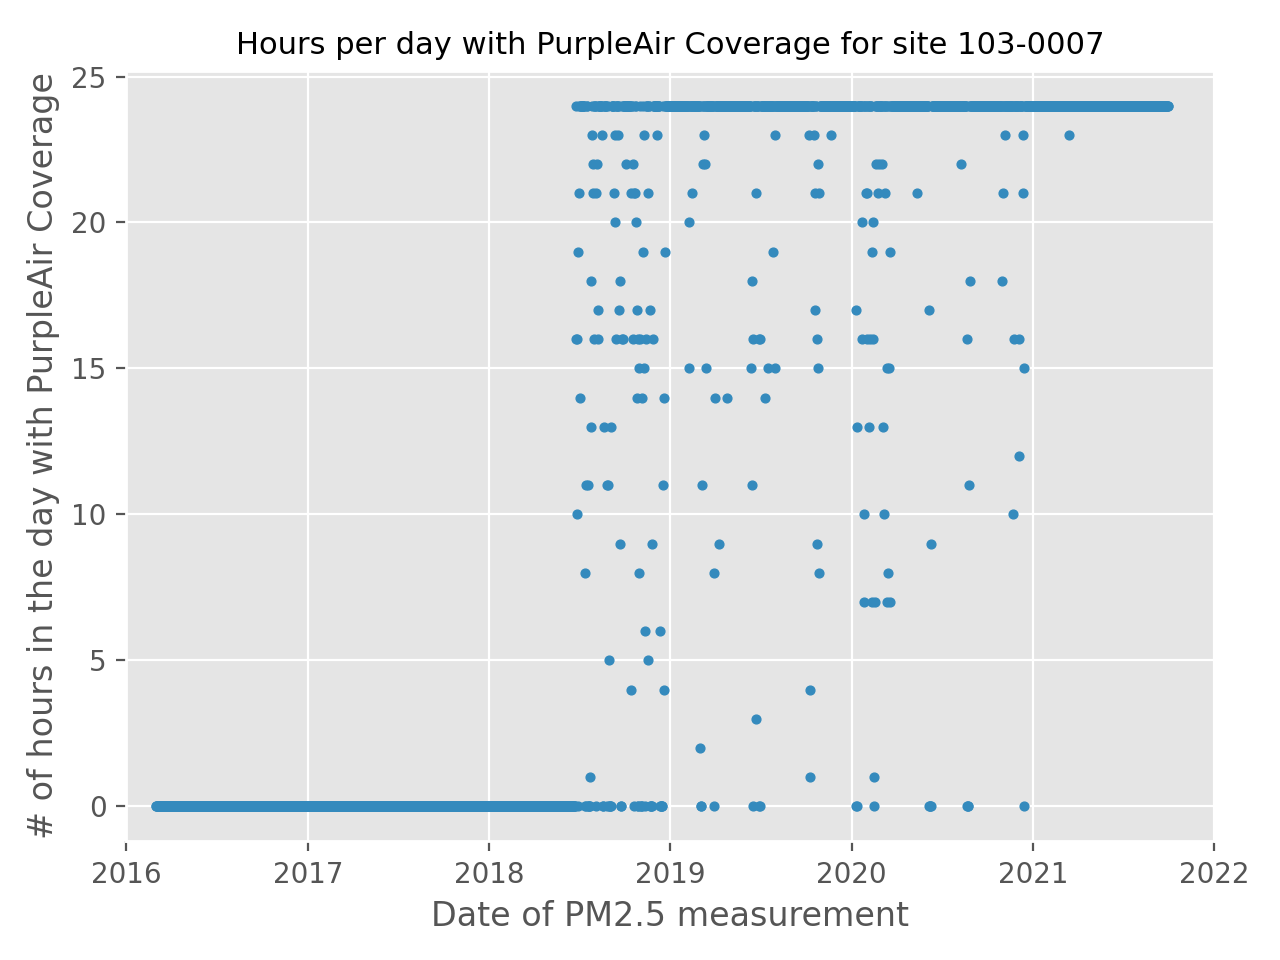
\includegraphics[width=0.8\textwidth]{appendix/site_plots/site-103-0007_pa-daily-covereage.png}
\caption{Scatter plot indicating the number of hours in each day that this NAAQS monitor has PurpleAir coverage. An hour has PurpleAir coverage if there are any PurpleAir sensor readings within the 5-mile radius of the monitor site for that hour. The weighted average is calculated for that hour using all the available PurpleAir readings within 5 miles. This monitor is at site 0007 in county 103 (FIPS code).}
\label{fig:hourly_coverage_103-0007}
\end{figure}
%=========================================
%  PurpleAir EPA Non-missing Comparison
%=========================================
\begin{figure}
\centering
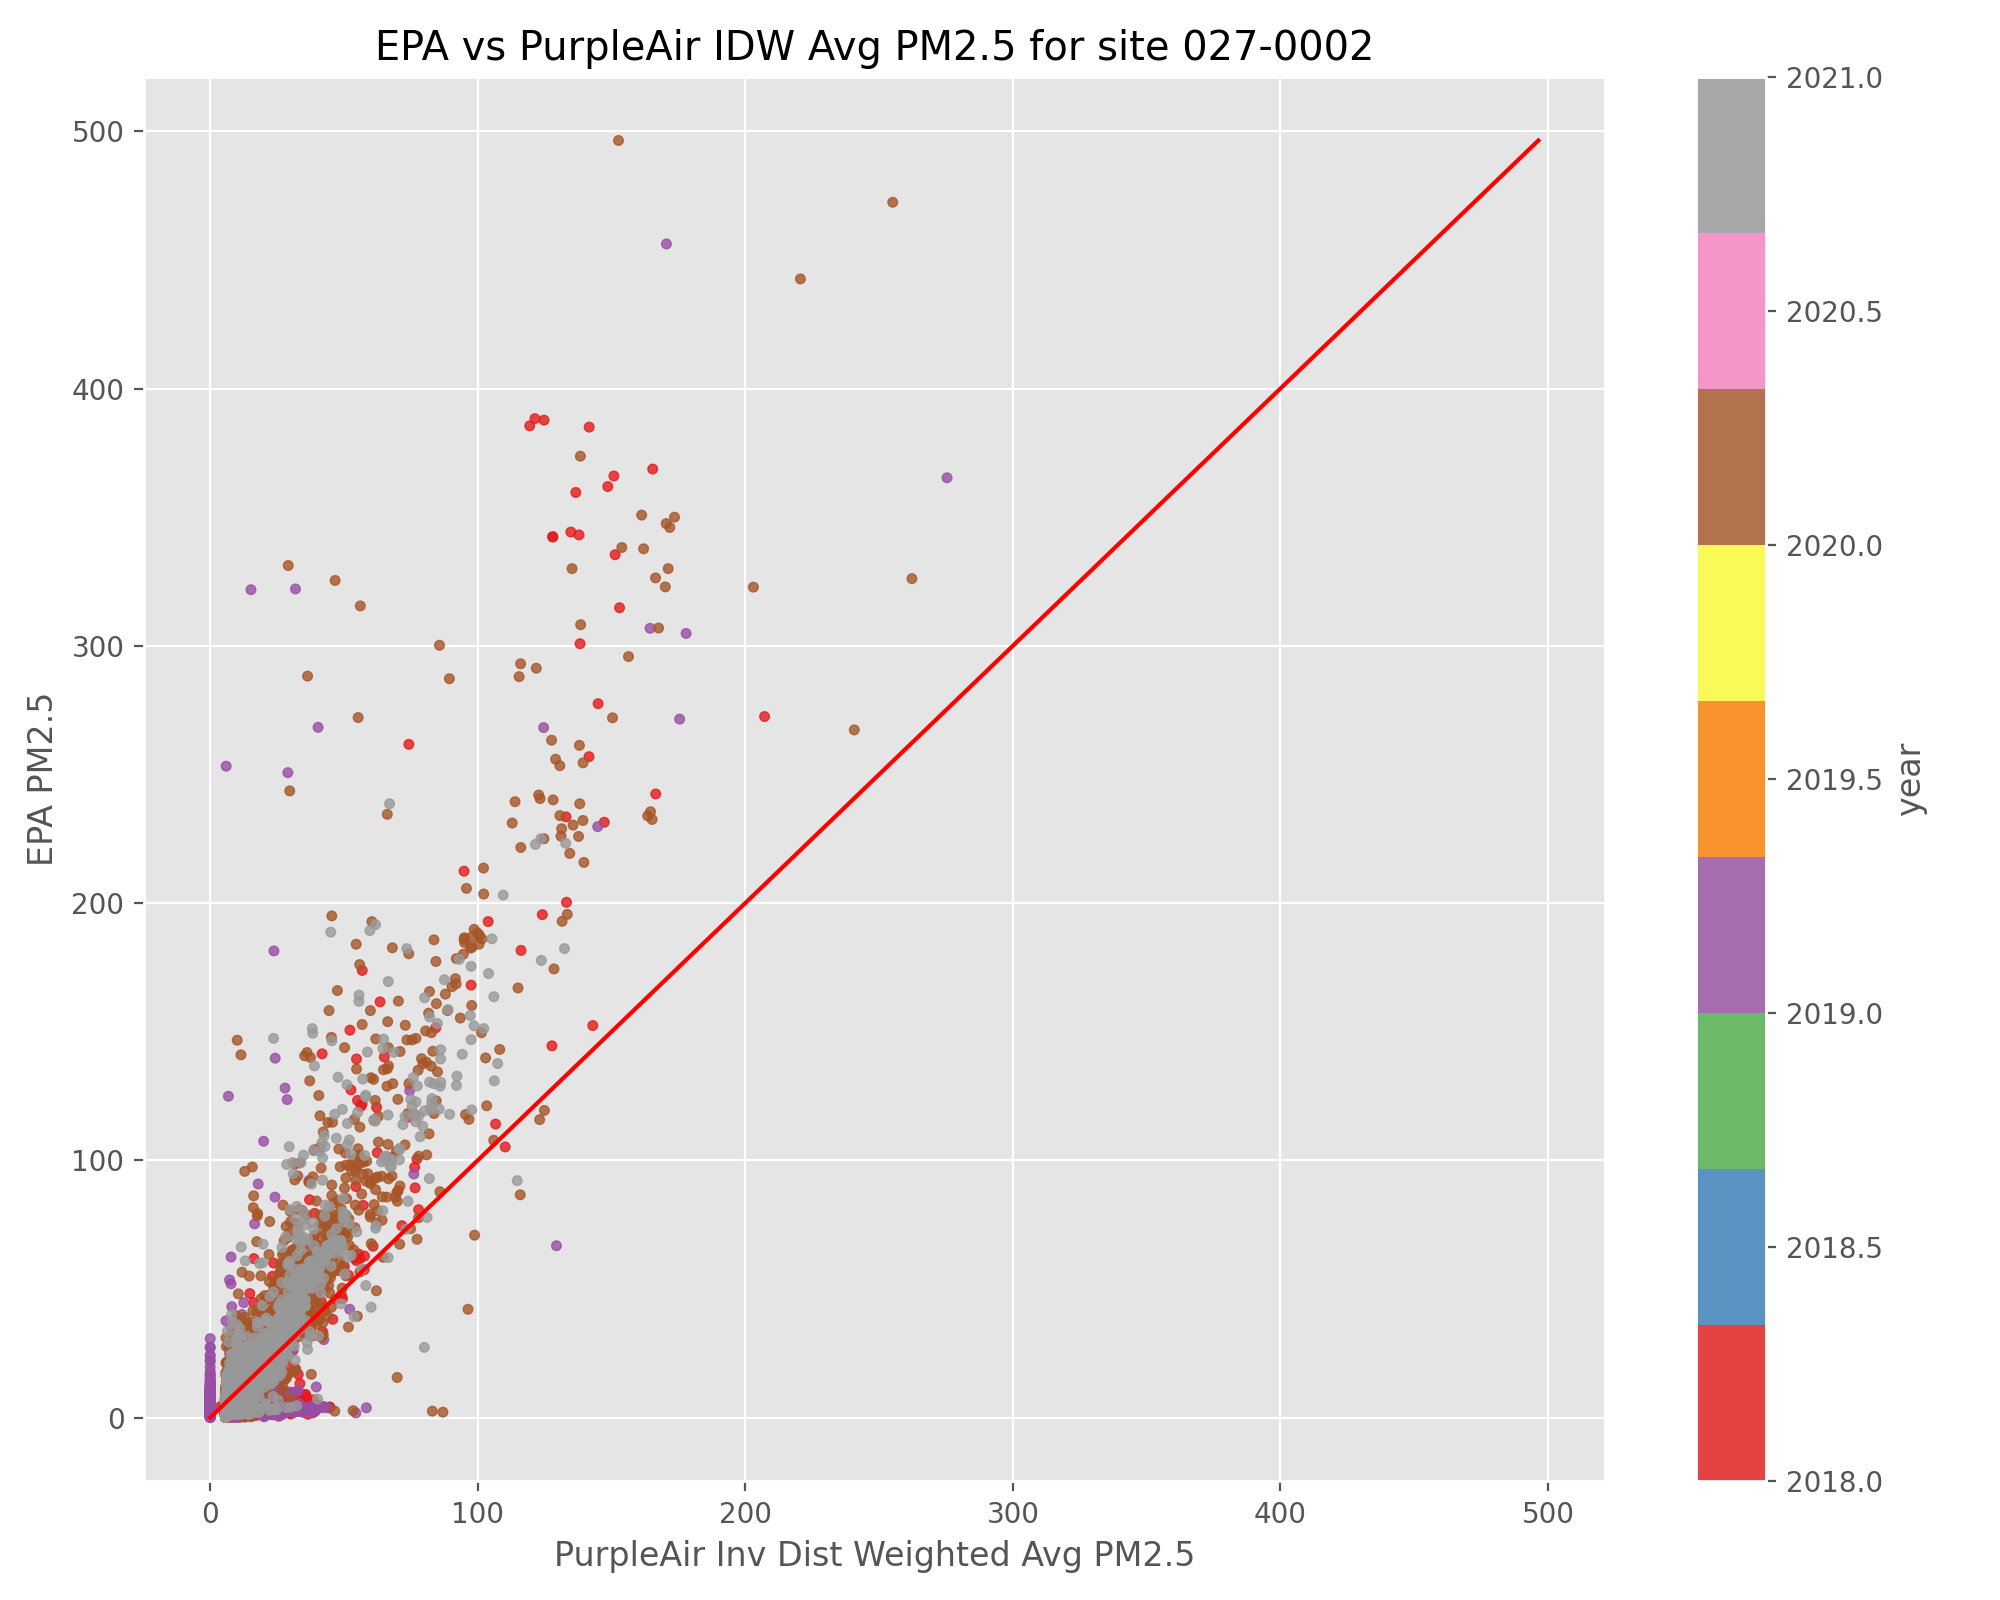
\includegraphics[width=0.8\textwidth]{appendix/site_plots/site-027-0002_epa-pa-hourly-plot.png}
\caption{Scatter plot comparing reported hourly PM2.5 measurements: the x-axis represents the IDW-weighted average of PurpleAir measurements, the y-axis represents reported NAAQS-primary monitor measurements. The red line is a 45$^\circ$ line, representing perfect correlation between the PurpleAir average and the NAAQS-primary monitor. This monitor is at site 0002 in county 027 (FIPS code).}
\label{fig:pa-epa-compare_027-0002}
\end{figure}
\begin{figure}
\centering
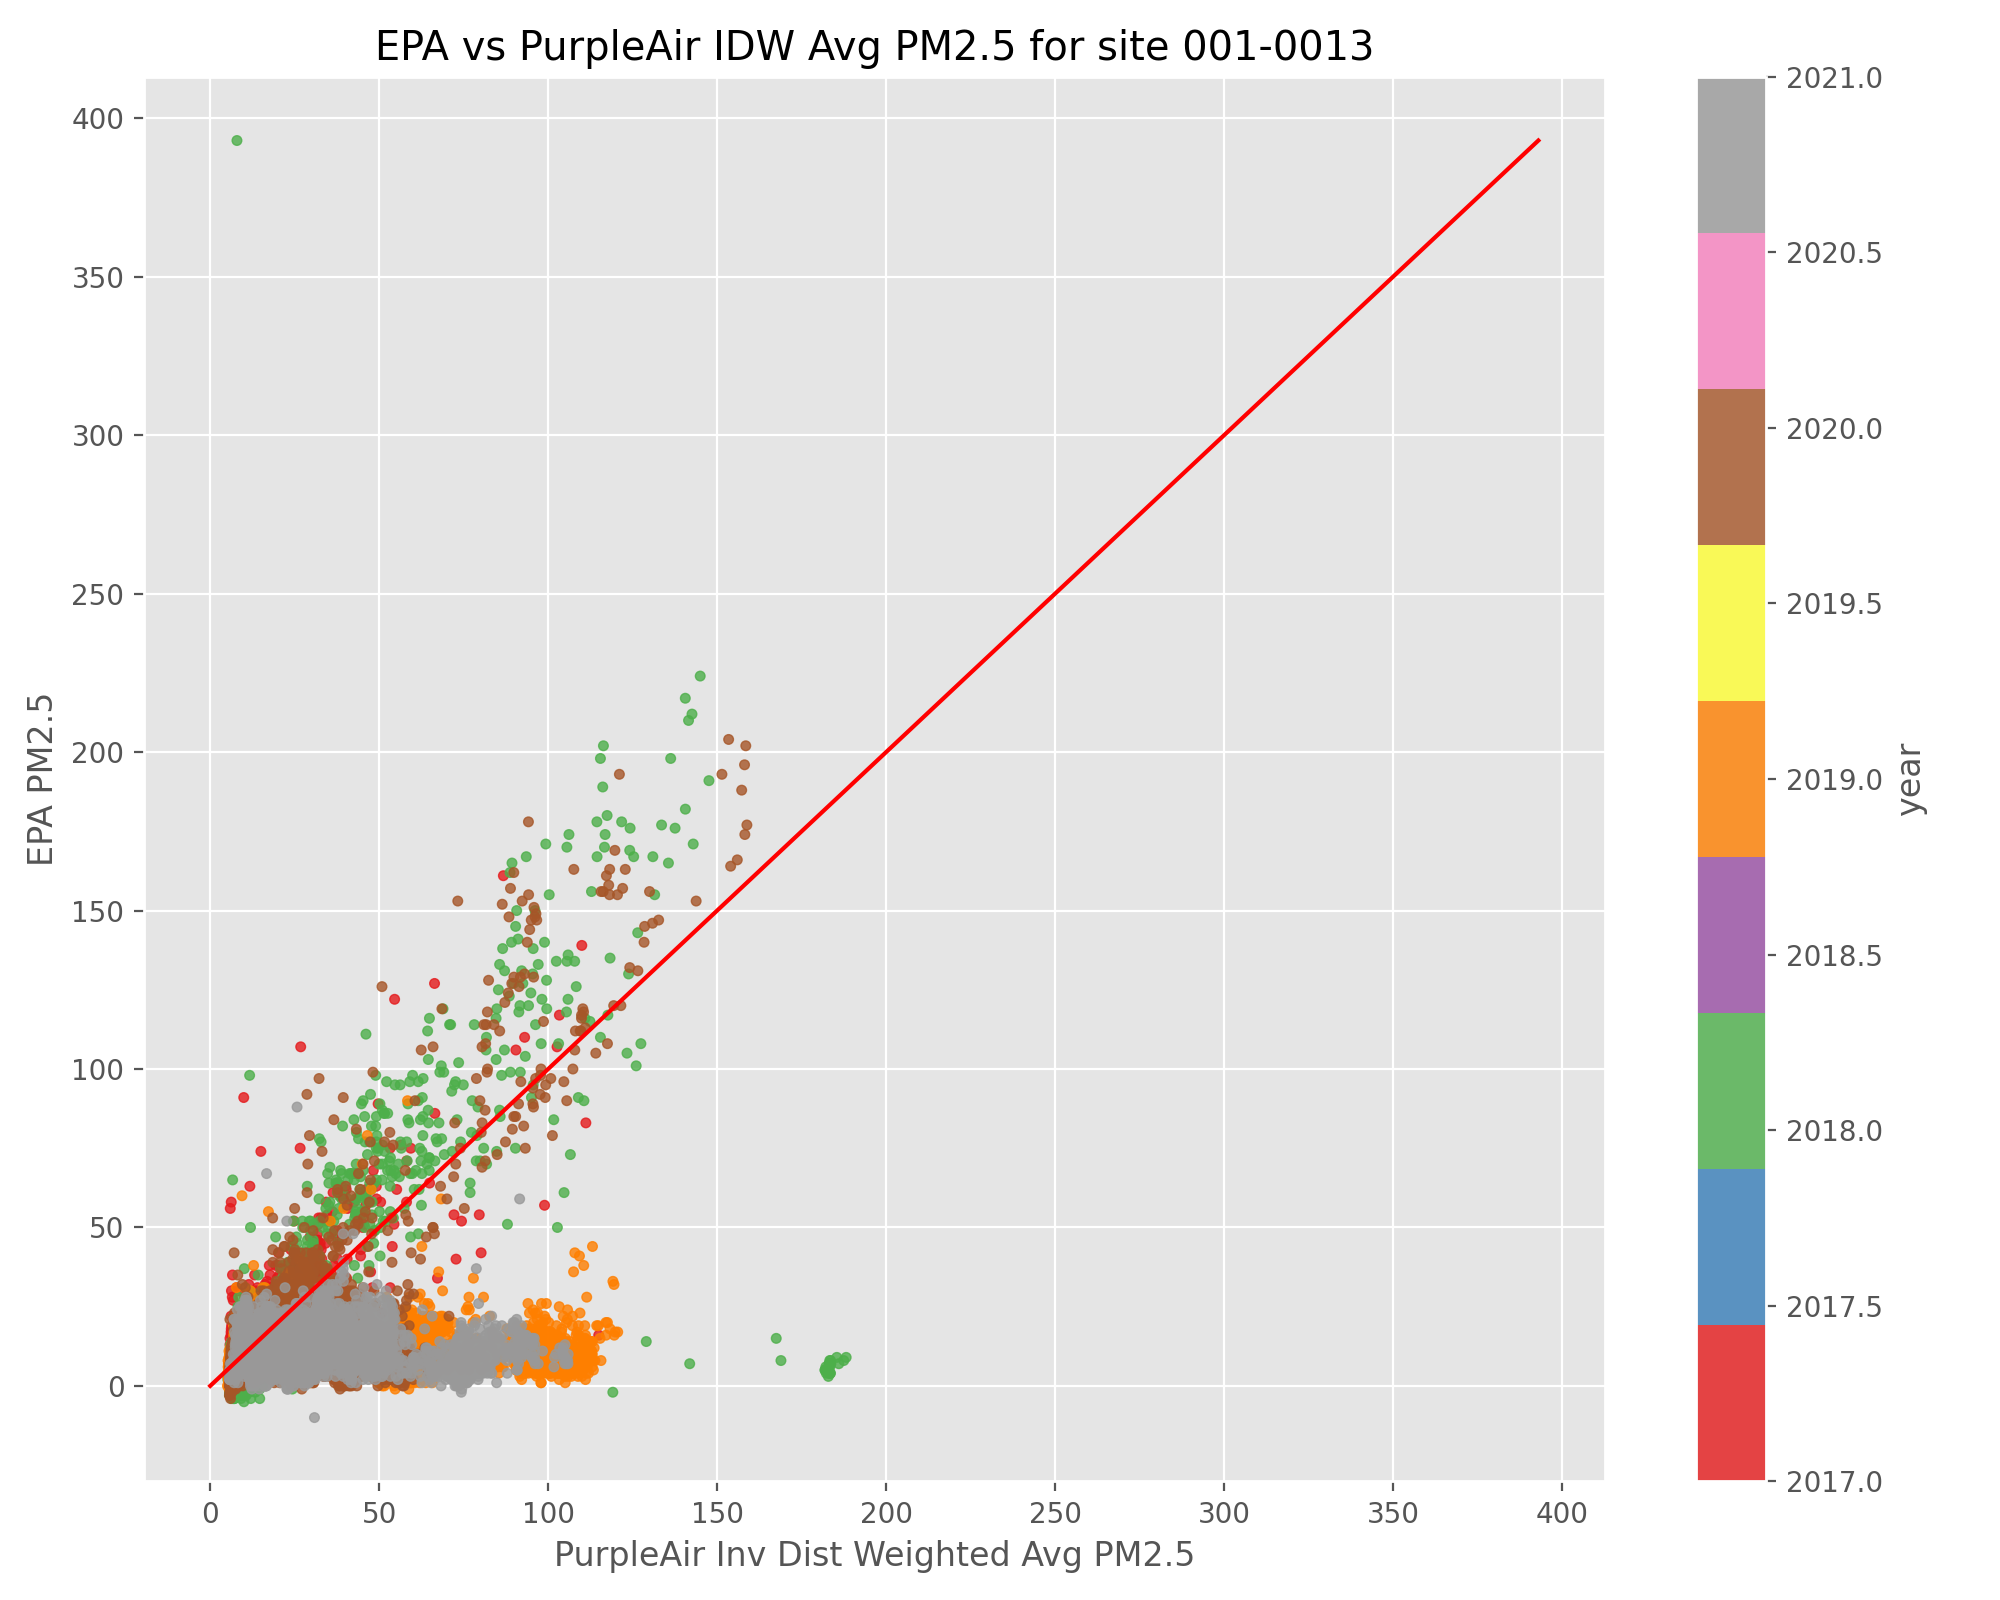
\includegraphics[width=0.8\textwidth]{appendix/site_plots/site-001-0013_epa-pa-hourly-plot.png}
\caption{Scatter plot comparing reported hourly PM2.5 measurements: the x-axis represents the IDW-weighted average of PurpleAir measurements, the y-axis represents reported NAAQS-primary monitor measurements. The red line is a 45$^\circ$ line, representing perfect correlation between the PurpleAir average and the NAAQS-primary monitor. This monitor is at site 0013 in county 001 (FIPS code).}
\label{fig:pa-epa-compare_001-0013}
\end{figure}
\begin{figure}
\centering
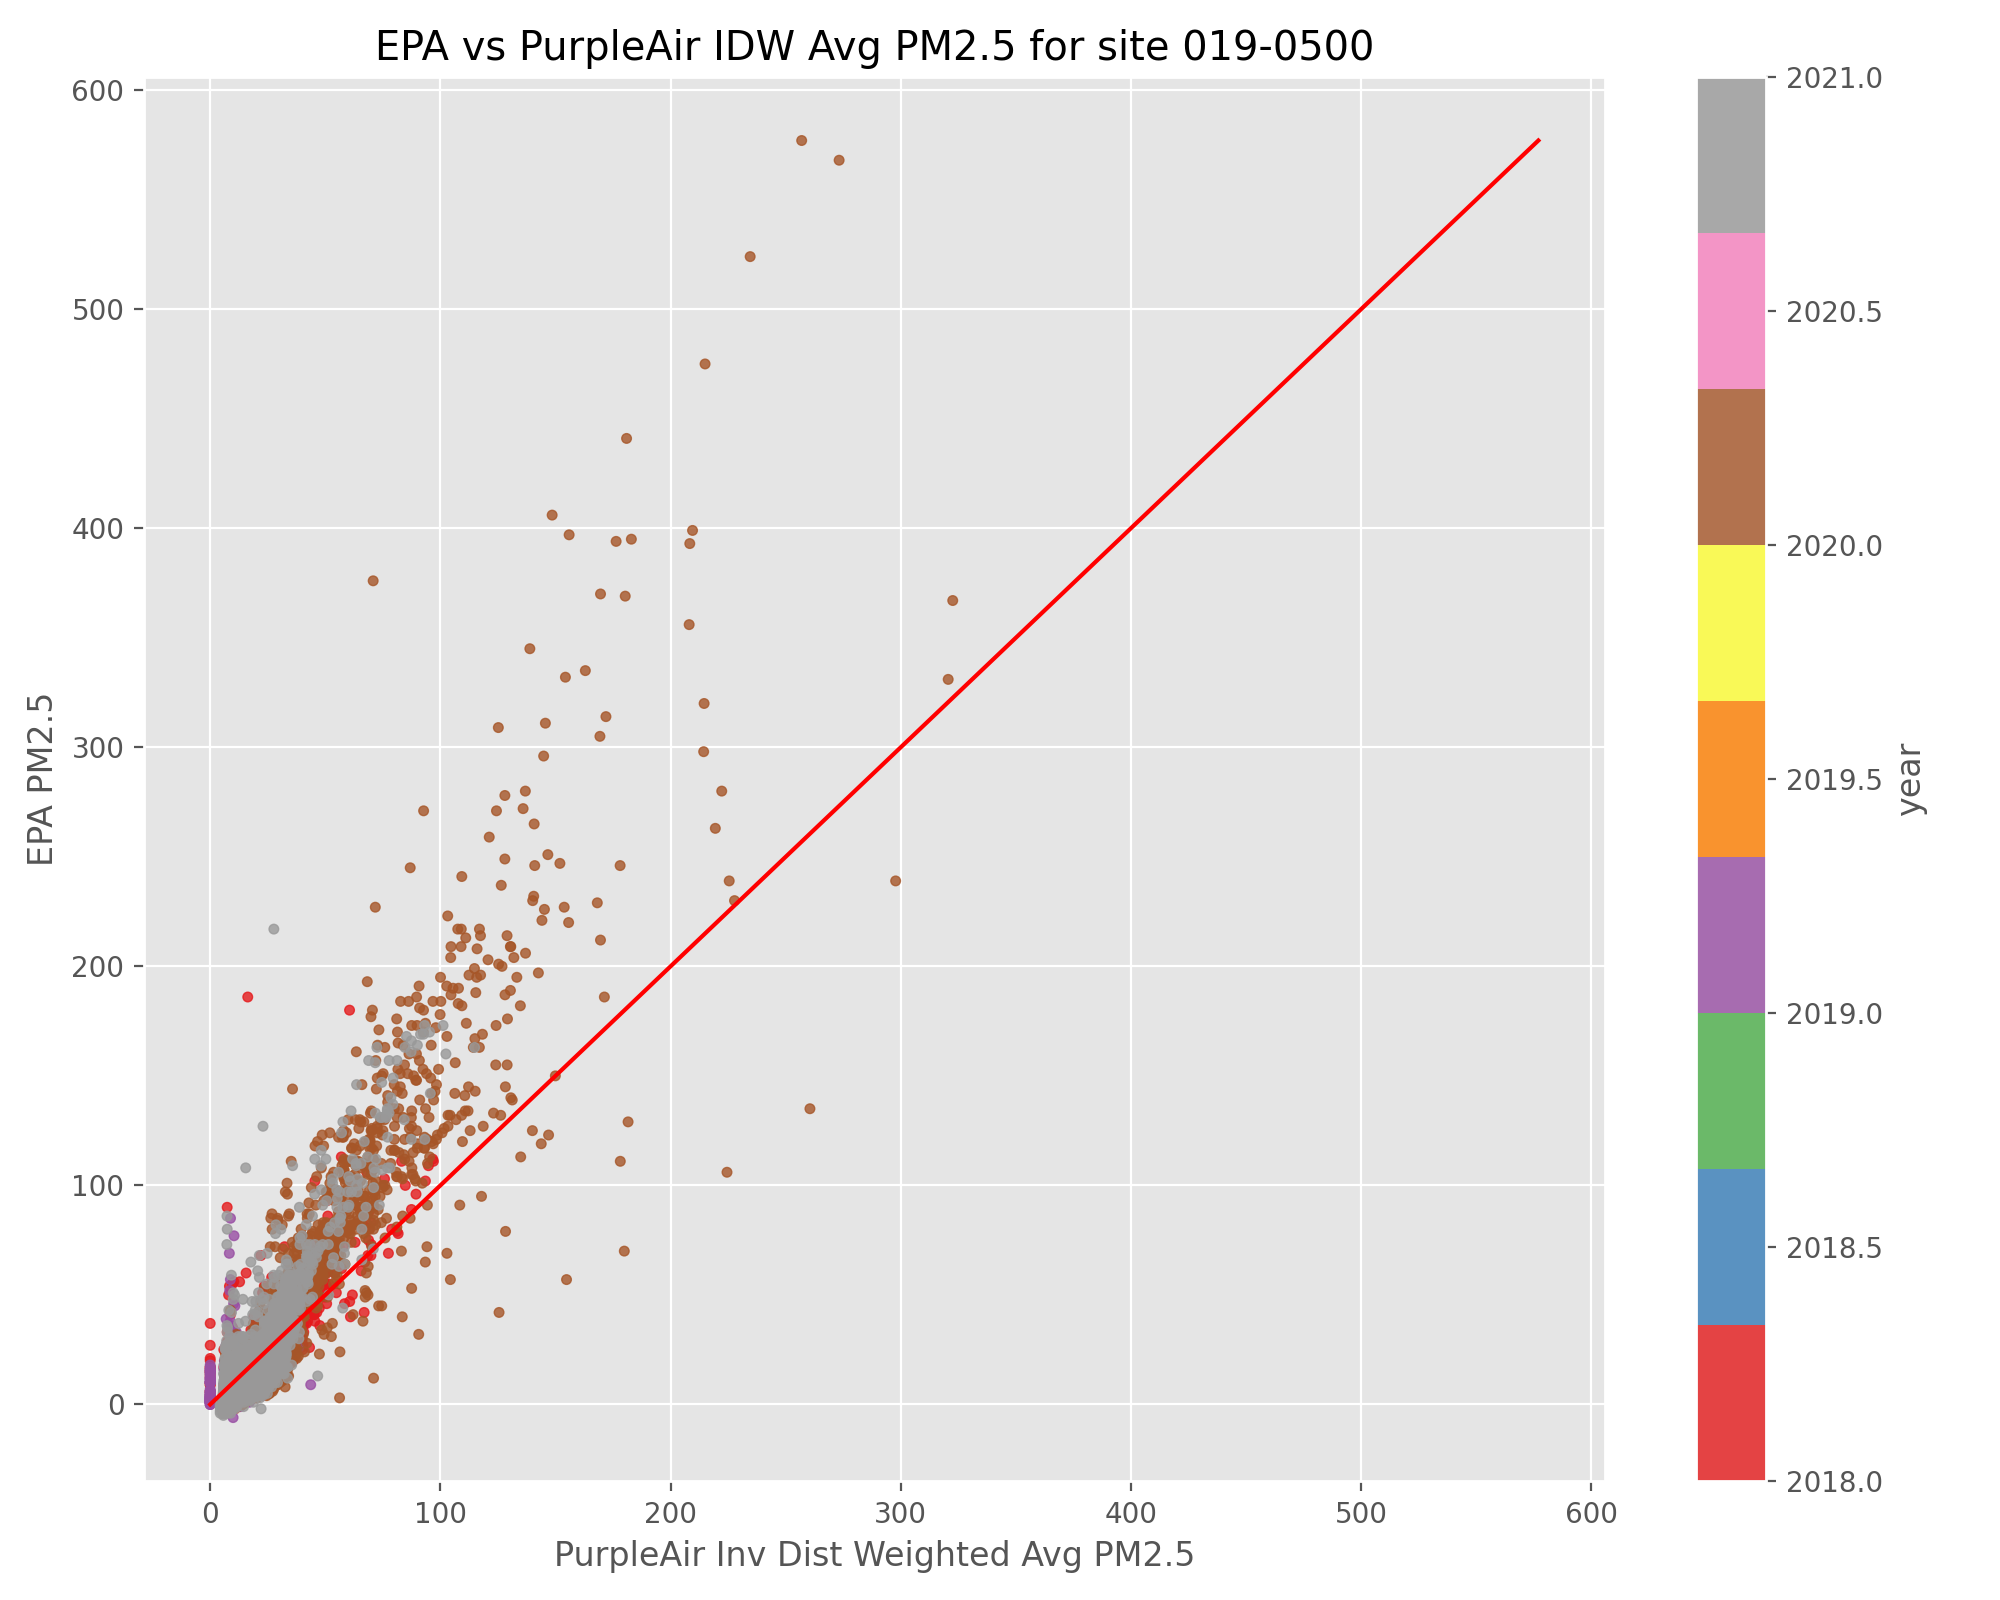
\includegraphics[width=0.8\textwidth]{appendix/site_plots/site-019-0500_epa-pa-hourly-plot.png}
\caption{Scatter plot comparing reported hourly PM2.5 measurements: the x-axis represents the IDW-weighted average of PurpleAir measurements, the y-axis represents reported NAAQS-primary monitor measurements. The red line is a 45$^\circ$ line, representing perfect correlation between the PurpleAir average and the NAAQS-primary monitor. This monitor is at site 0500 in county 019 (FIPS code).}
\label{fig:pa-epa-compare_019-0500}
\end{figure}
\begin{figure}
\centering
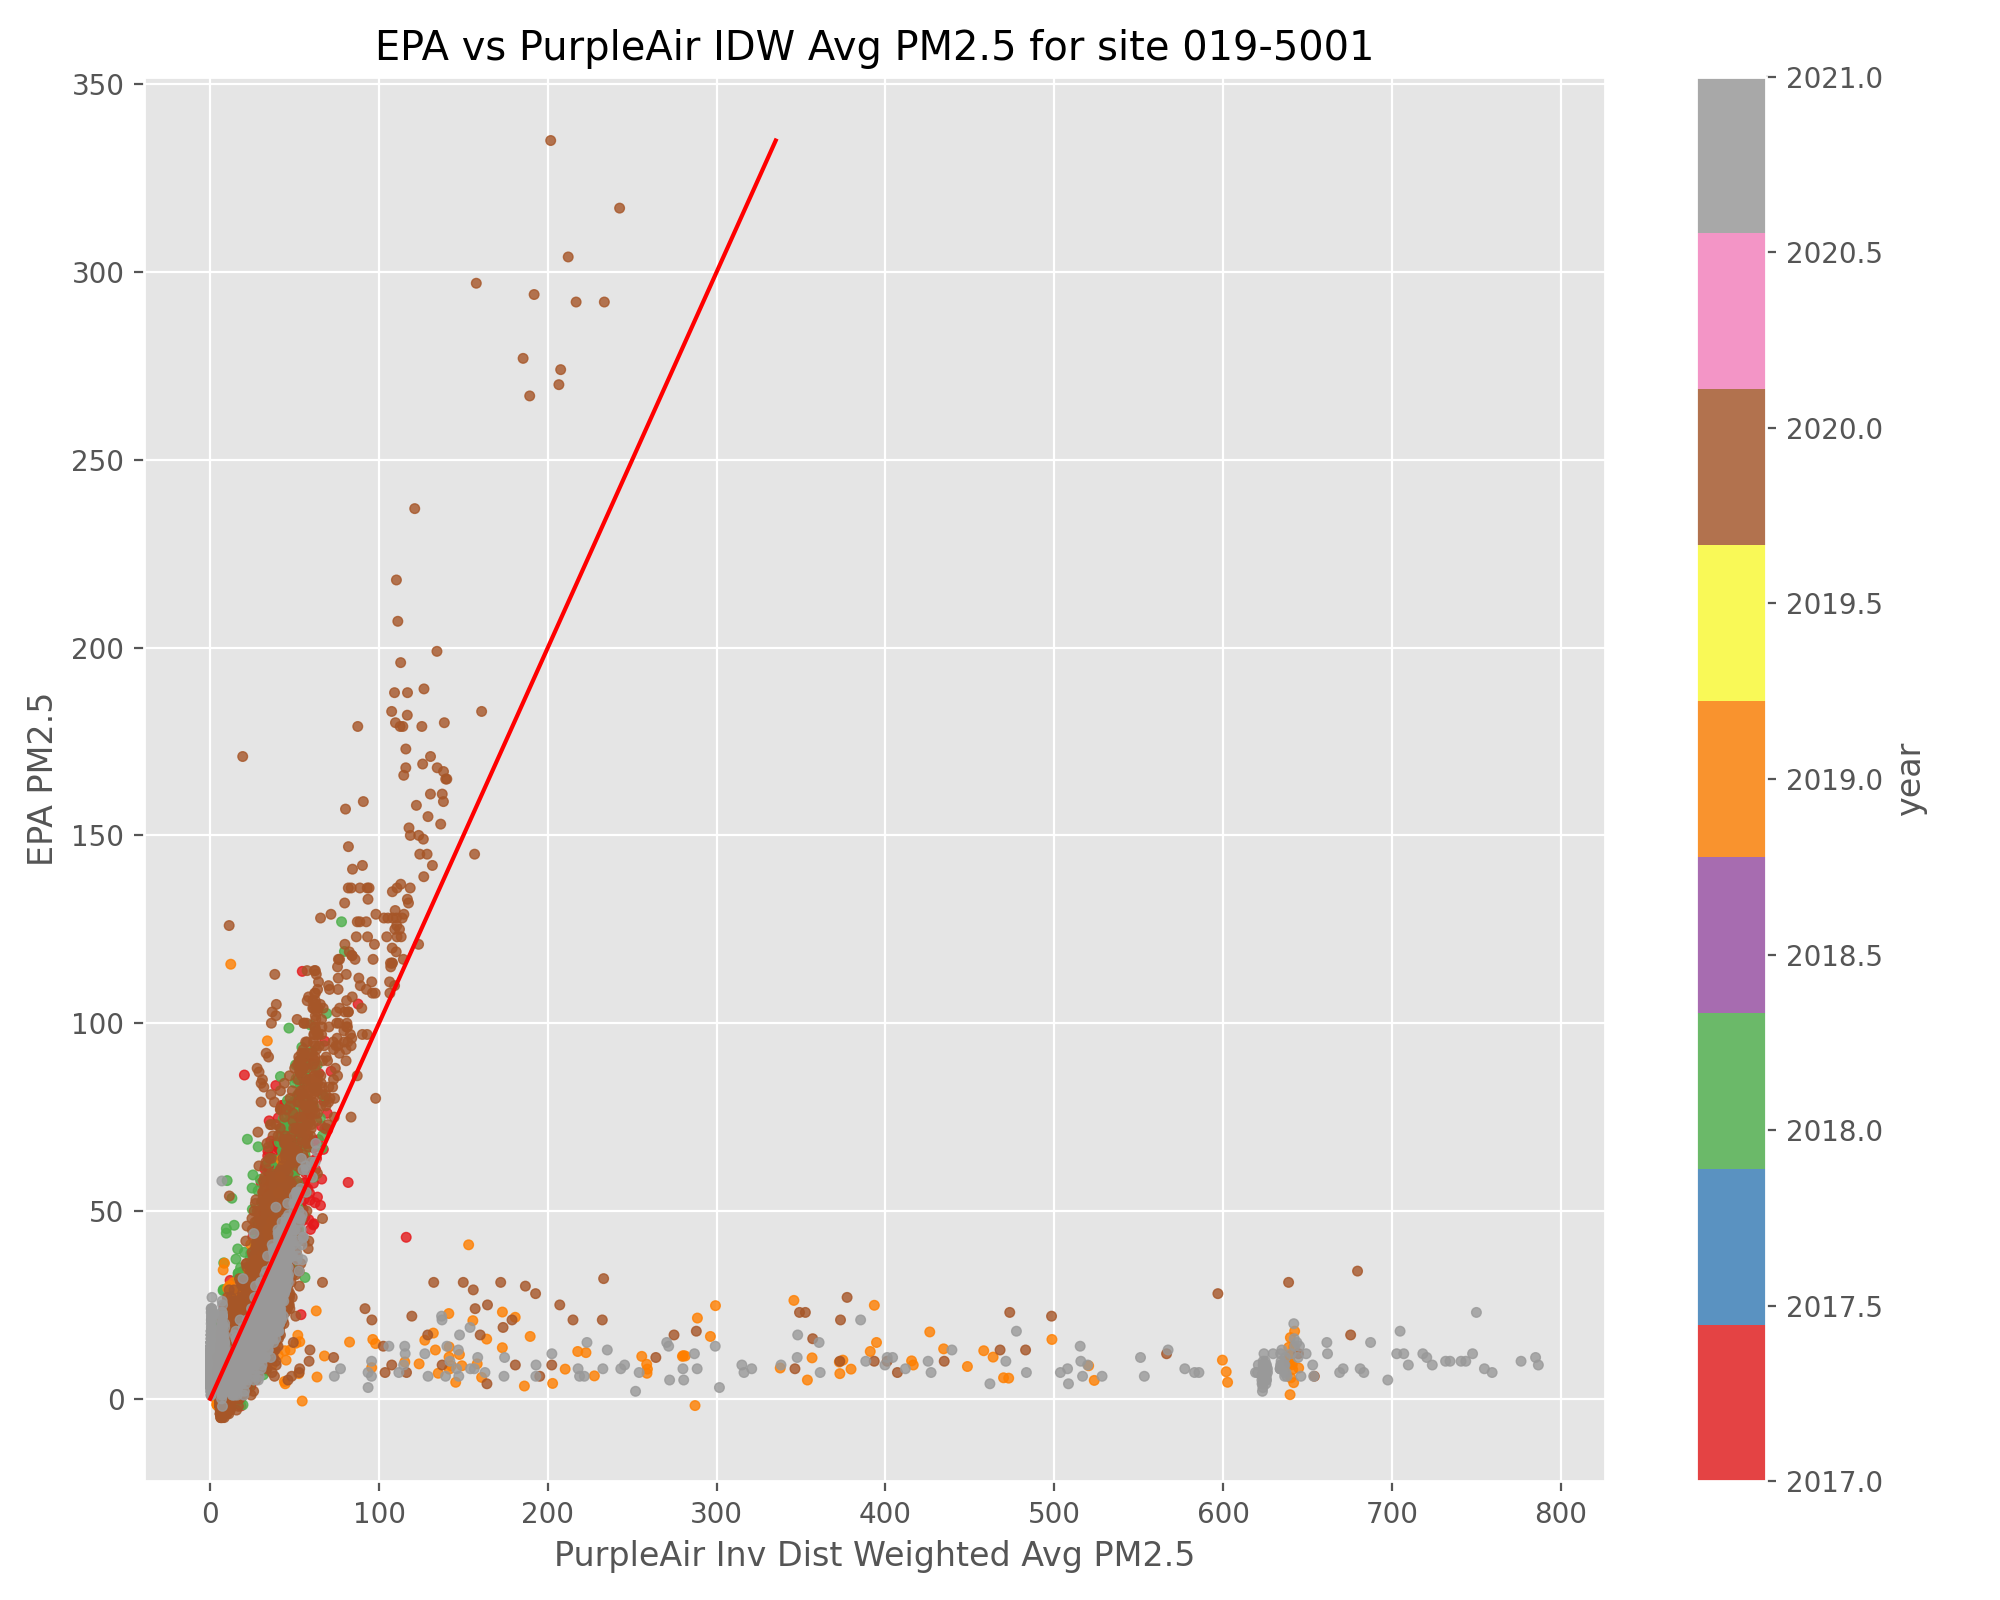
\includegraphics[width=0.8\textwidth]{appendix/site_plots/site-019-5001_epa-pa-hourly-plot.png}
\caption{Scatter plot comparing reported hourly PM2.5 measurements: the x-axis represents the IDW-weighted average of PurpleAir measurements, the y-axis represents reported NAAQS-primary monitor measurements. The red line is a 45$^\circ$ line, representing perfect correlation between the PurpleAir average and the NAAQS-primary monitor. This monitor is at site 5001 in county 019 (FIPS code).}
\label{fig:pa-epa-compare_019-5001}
\end{figure}
\begin{figure}
\centering
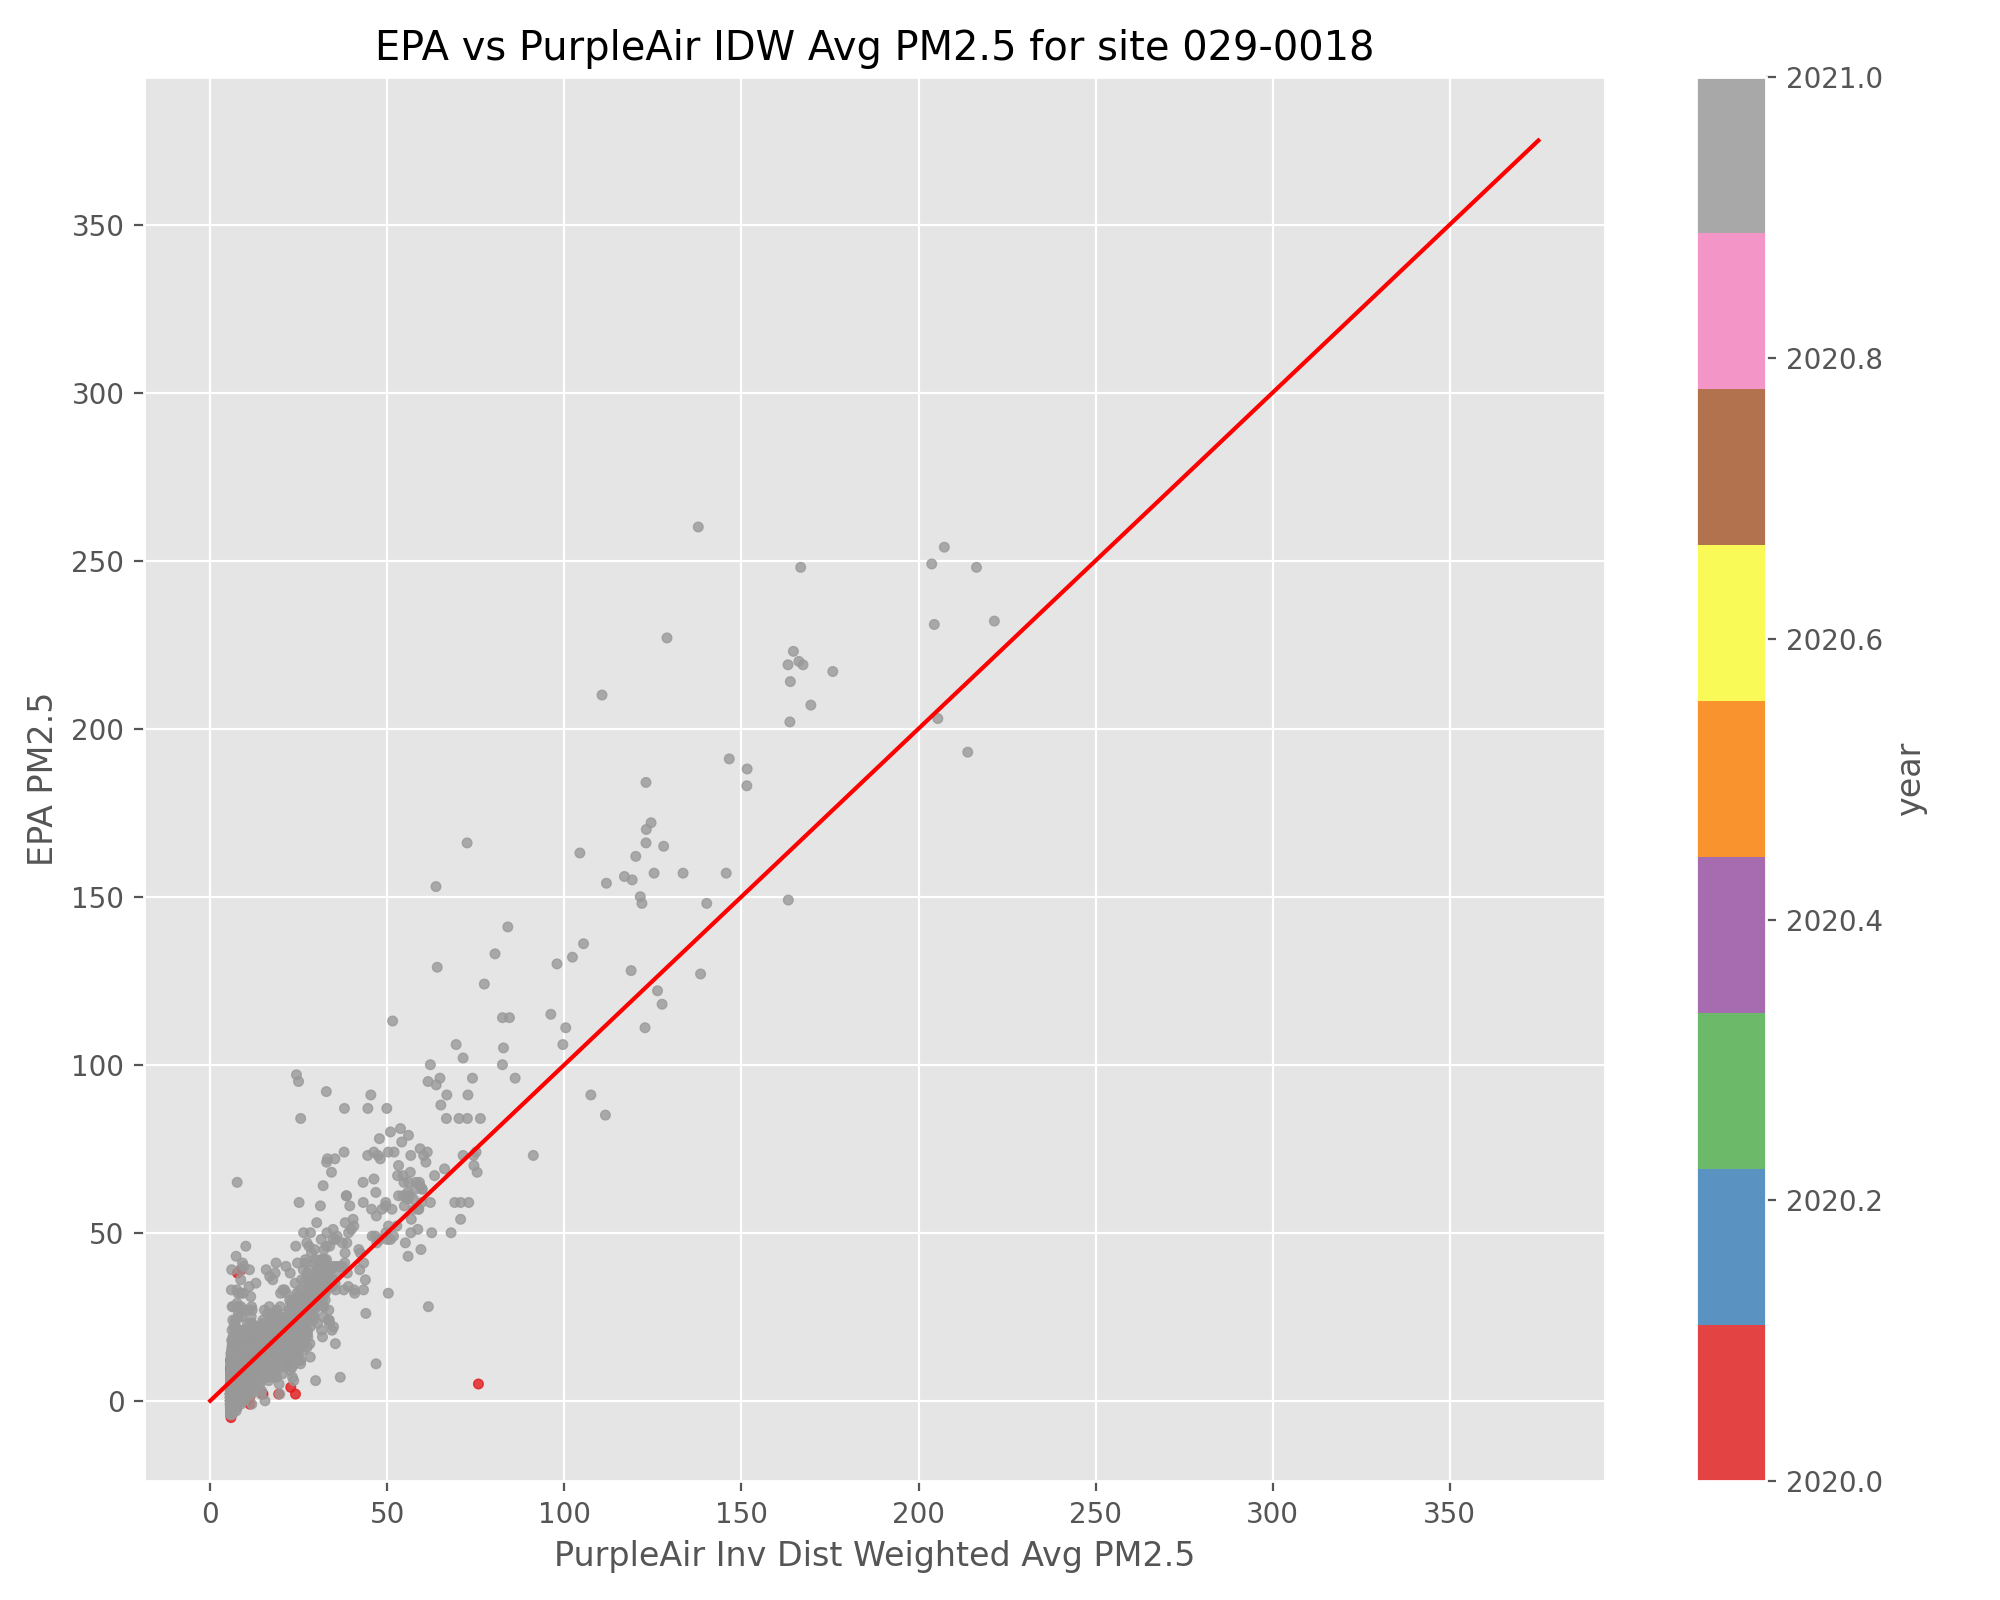
\includegraphics[width=0.8\textwidth]{appendix/site_plots/site-029-0018_epa-pa-hourly-plot.png}
\caption{Scatter plot comparing reported hourly PM2.5 measurements: the x-axis represents the IDW-weighted average of PurpleAir measurements, the y-axis represents reported NAAQS-primary monitor measurements. The red line is a 45$^\circ$ line, representing perfect correlation between the PurpleAir average and the NAAQS-primary monitor. This monitor is at site 0018 in county 029 (FIPS code).}
\label{fig:pa-epa-compare_029-0018}
\end{figure}
\begin{figure}
\centering
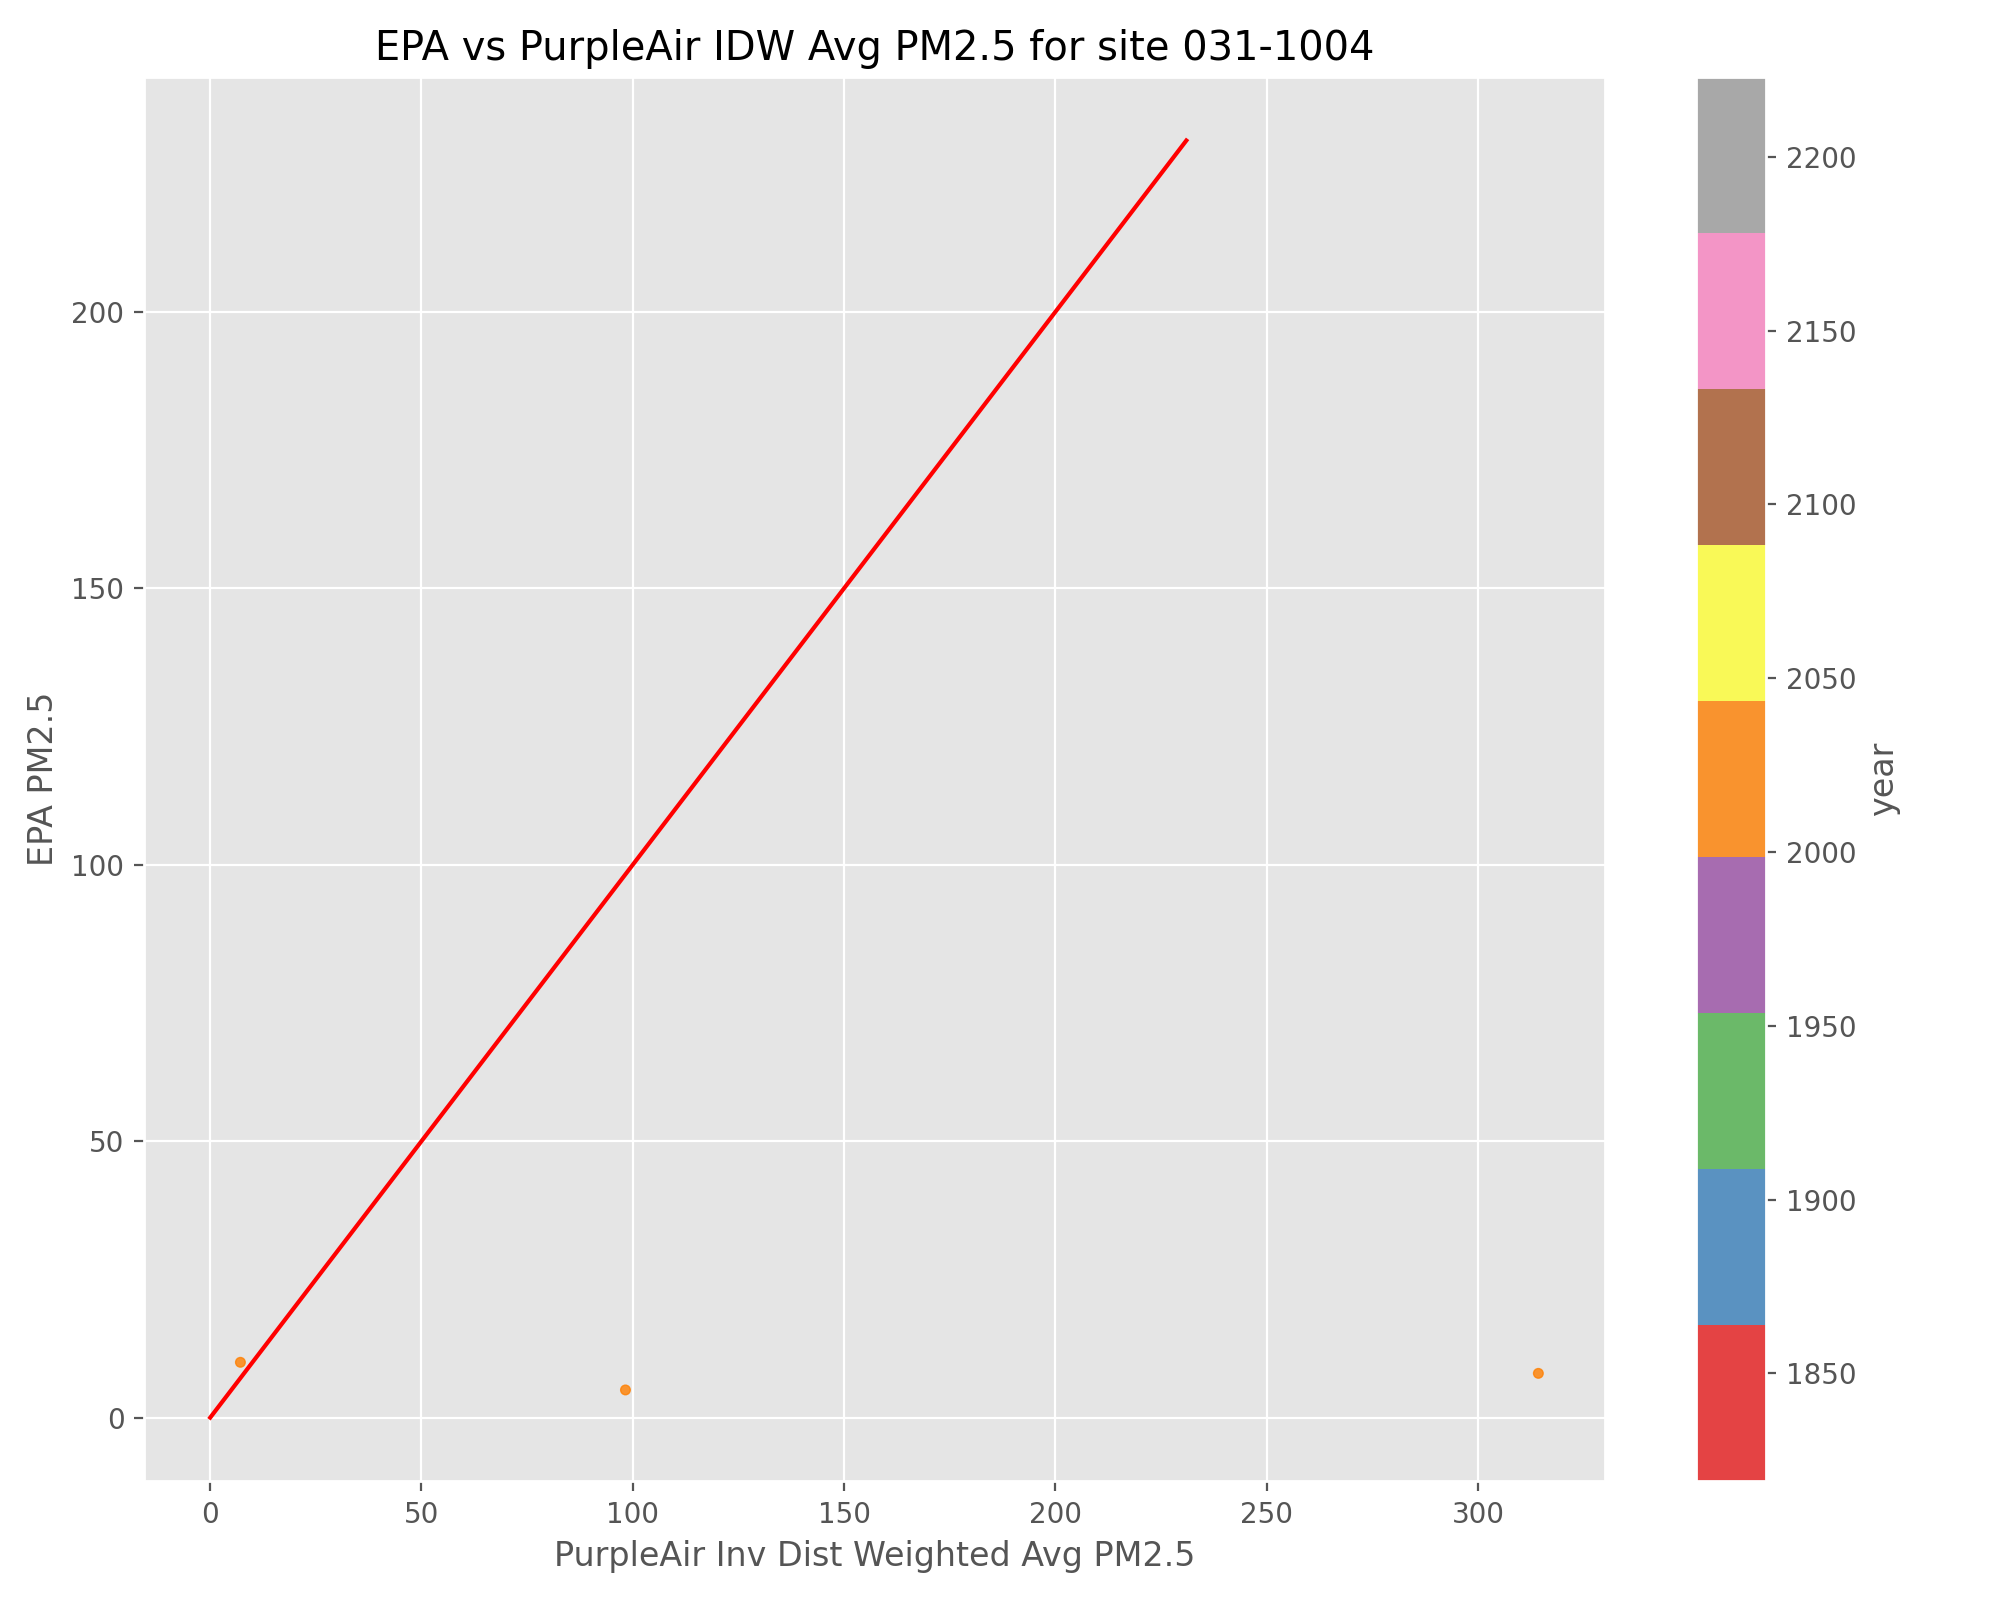
\includegraphics[width=0.8\textwidth]{appendix/site_plots/site-031-1004_epa-pa-hourly-plot.png}
\caption{Scatter plot comparing reported hourly PM2.5 measurements: the x-axis represents the IDW-weighted average of PurpleAir measurements, the y-axis represents reported NAAQS-primary monitor measurements. The red line is a 45$^\circ$ line, representing perfect correlation between the PurpleAir average and the NAAQS-primary monitor. This monitor is at site 1004 in county 031 (FIPS code).}
\label{fig:pa-epa-compare_031-1004}
\end{figure}
\begin{figure}
\centering
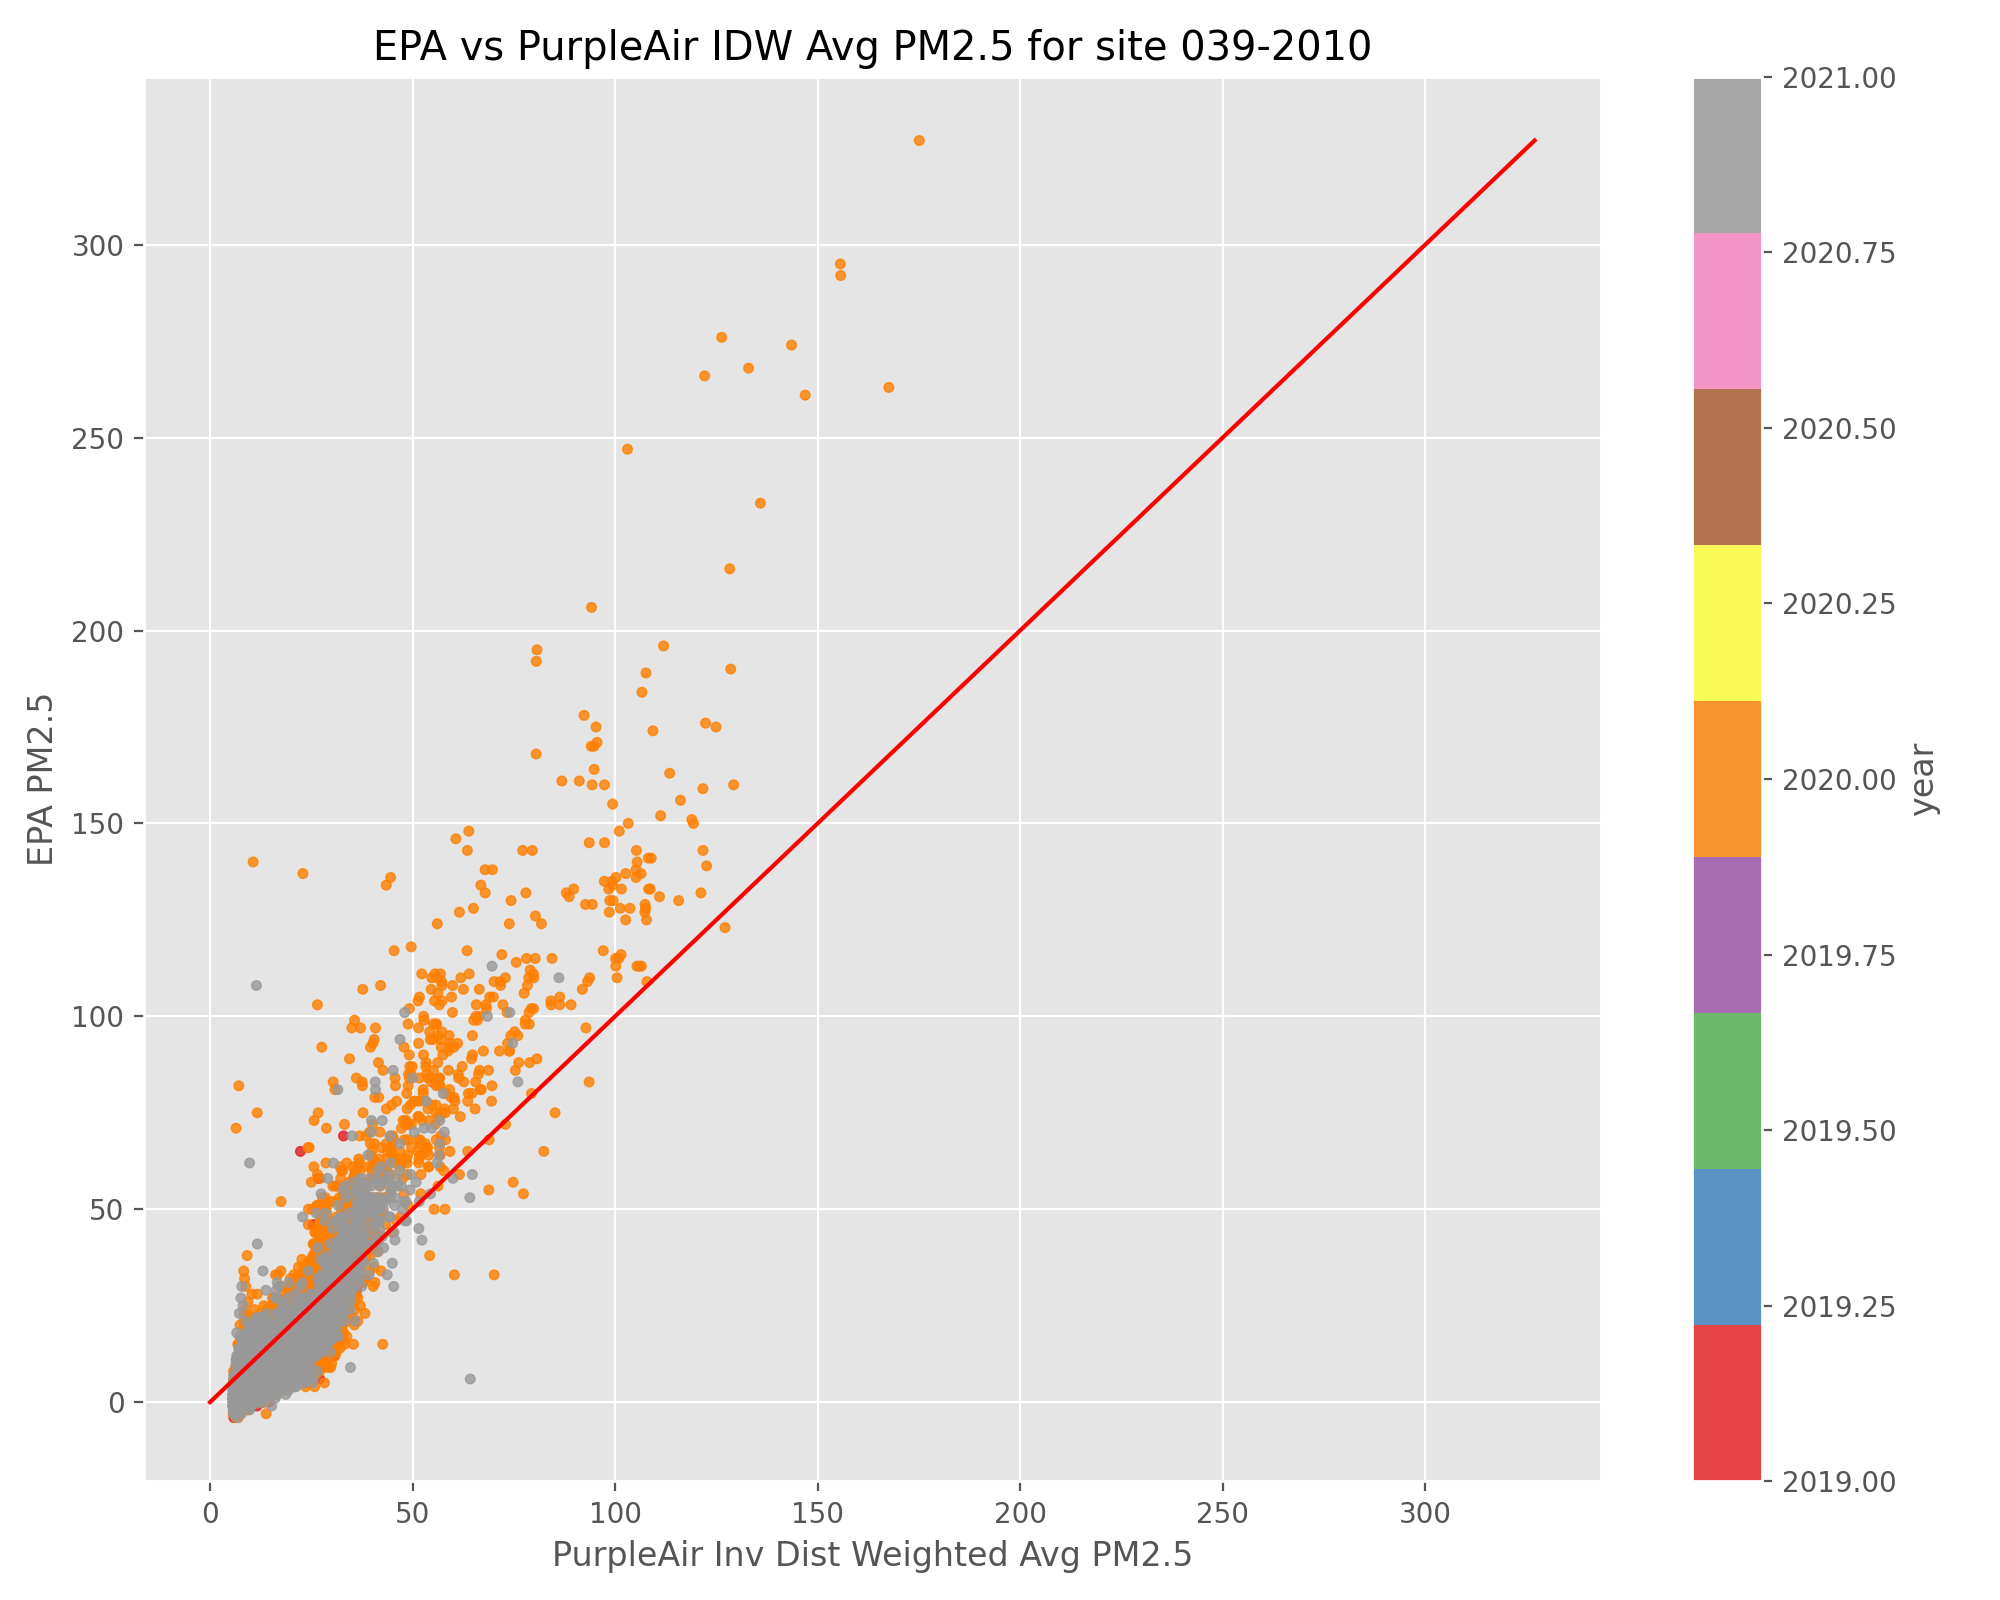
\includegraphics[width=0.8\textwidth]{appendix/site_plots/site-039-2010_epa-pa-hourly-plot.png}
\caption{Scatter plot comparing reported hourly PM2.5 measurements: the x-axis represents the IDW-weighted average of PurpleAir measurements, the y-axis represents reported NAAQS-primary monitor measurements. The red line is a 45$^\circ$ line, representing perfect correlation between the PurpleAir average and the NAAQS-primary monitor. This monitor is at site 2010 in county 039 (FIPS code).}
\label{fig:pa-epa-compare_039-2010}
\end{figure}
\begin{figure}
\centering
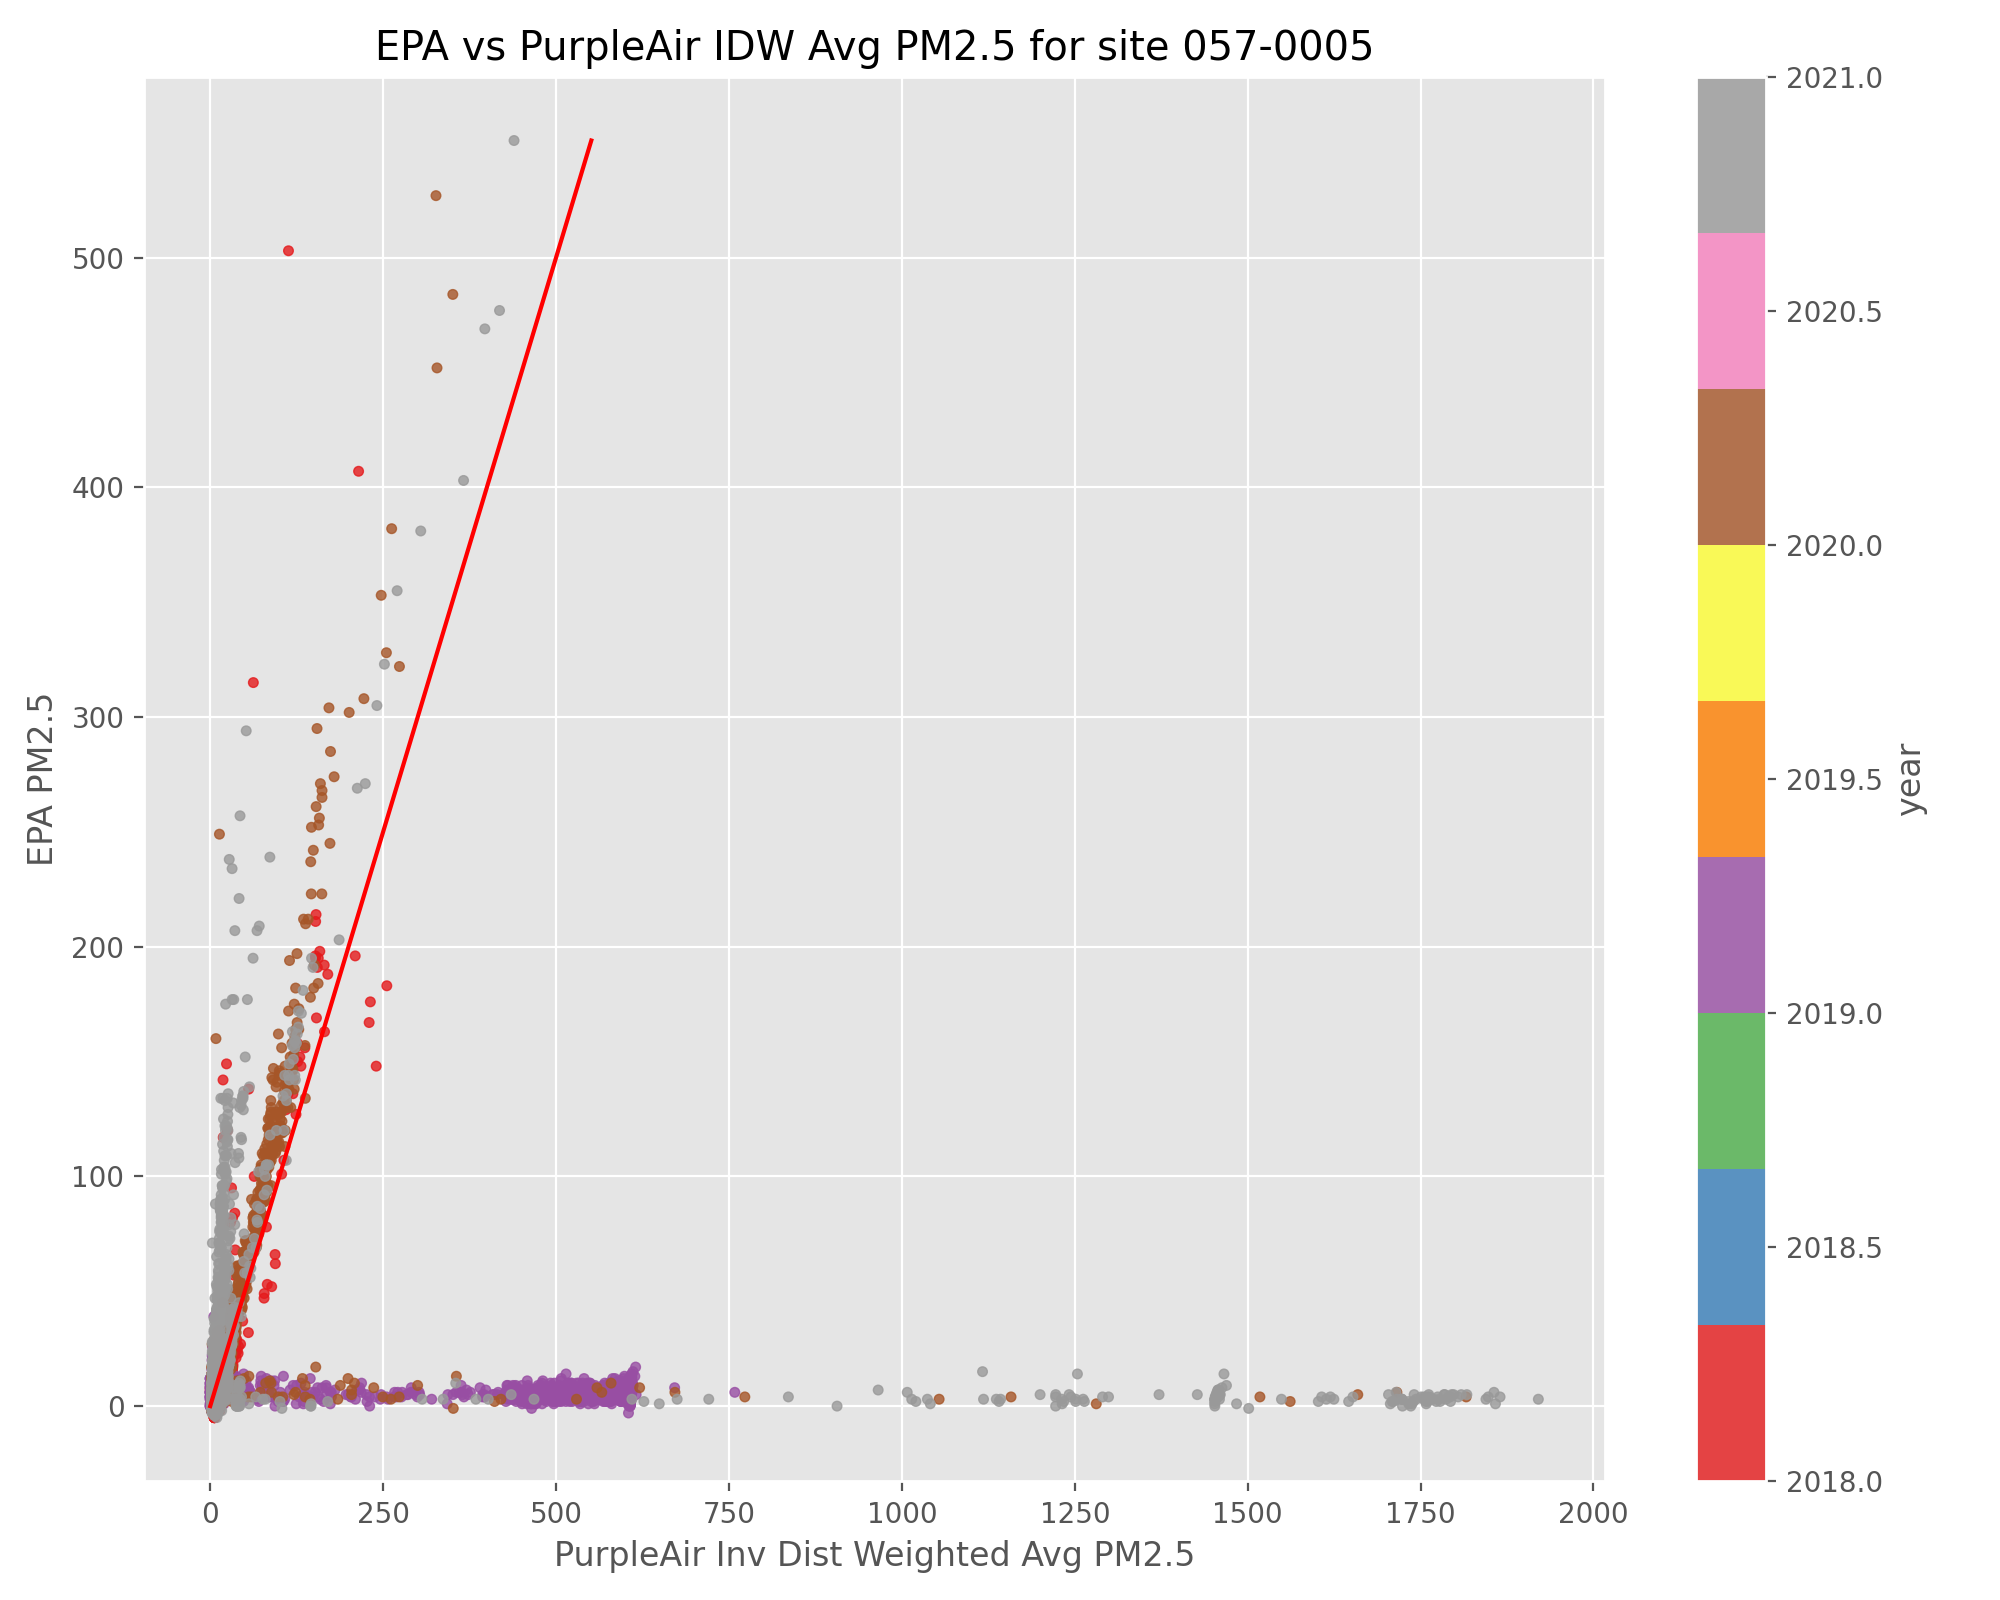
\includegraphics[width=0.8\textwidth]{appendix/site_plots/site-057-0005_epa-pa-hourly-plot.png}
\caption{Scatter plot comparing reported hourly PM2.5 measurements: the x-axis represents the IDW-weighted average of PurpleAir measurements, the y-axis represents reported NAAQS-primary monitor measurements. The red line is a 45$^\circ$ line, representing perfect correlation between the PurpleAir average and the NAAQS-primary monitor. This monitor is at site 0005 in county 057 (FIPS code).}
\label{fig:pa-epa-compare_057-0005}
\end{figure}
\begin{figure}
\centering
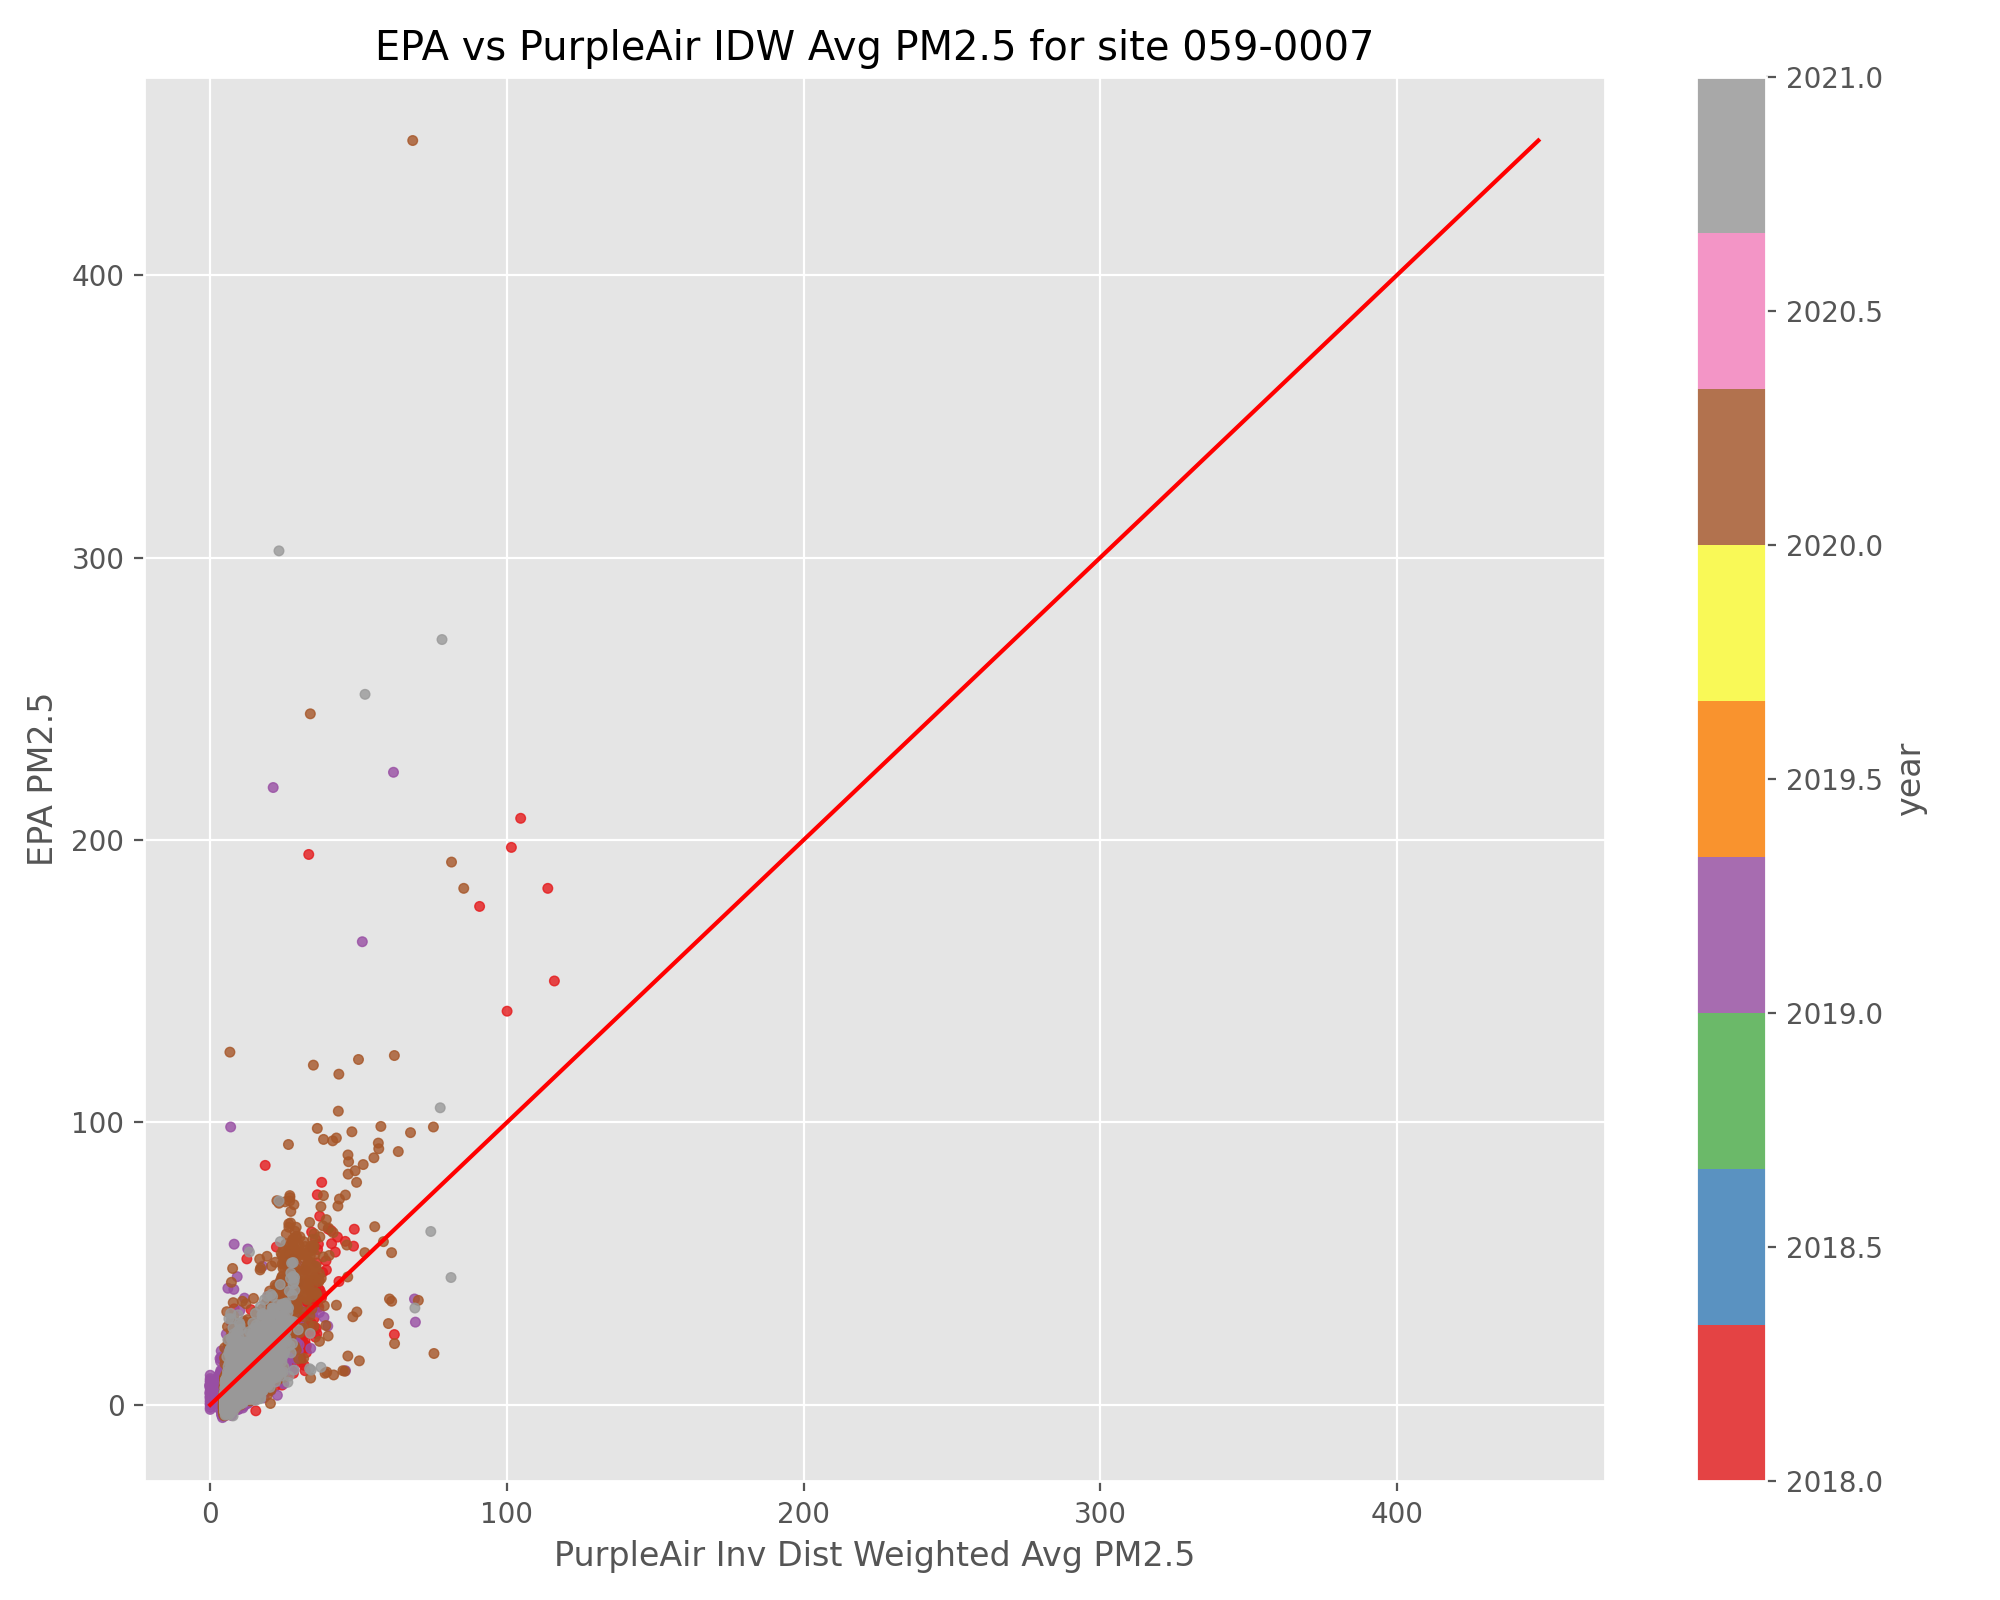
\includegraphics[width=0.8\textwidth]{appendix/site_plots/site-059-0007_epa-pa-hourly-plot.png}
\caption{Scatter plot comparing reported hourly PM2.5 measurements: the x-axis represents the IDW-weighted average of PurpleAir measurements, the y-axis represents reported NAAQS-primary monitor measurements. The red line is a 45$^\circ$ line, representing perfect correlation between the PurpleAir average and the NAAQS-primary monitor. This monitor is at site 0007 in county 059 (FIPS code).}
\label{fig:pa-epa-compare_059-0007}
\end{figure}
\begin{figure}
\centering
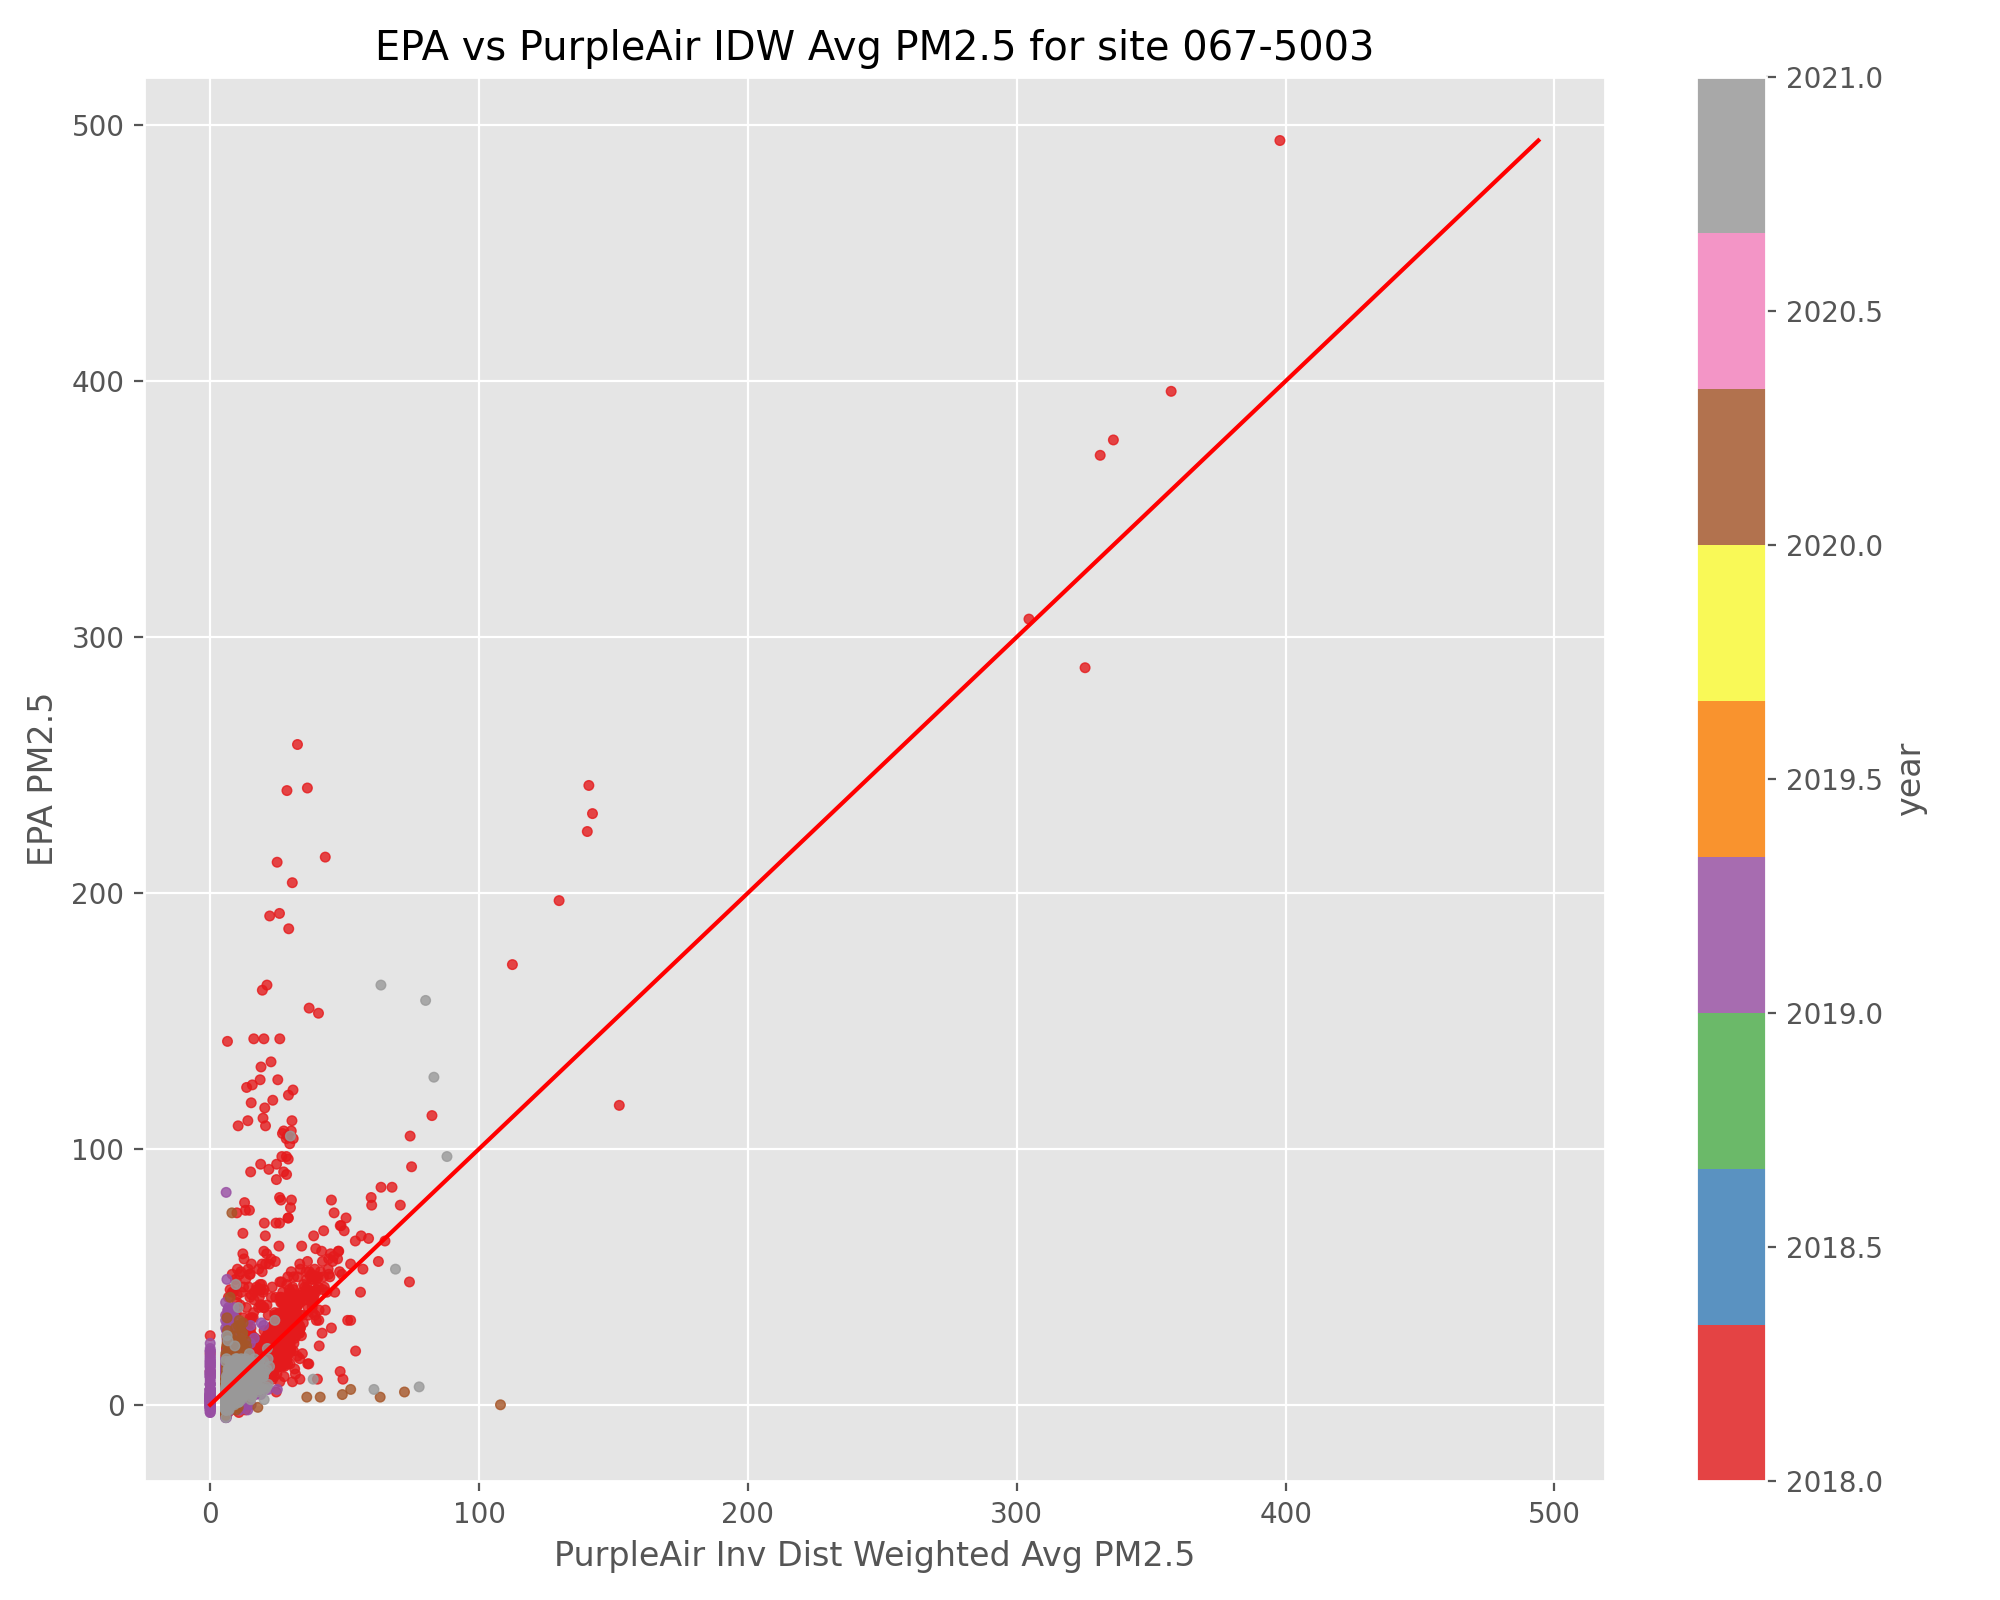
\includegraphics[width=0.8\textwidth]{appendix/site_plots/site-067-5003_epa-pa-hourly-plot.png}
\caption{Scatter plot comparing reported hourly PM2.5 measurements: the x-axis represents the IDW-weighted average of PurpleAir measurements, the y-axis represents reported NAAQS-primary monitor measurements. The red line is a 45$^\circ$ line, representing perfect correlation between the PurpleAir average and the NAAQS-primary monitor. This monitor is at site 5003 in county 067 (FIPS code).}
\label{fig:pa-epa-compare_067-5003}
\end{figure}
\begin{figure}
\centering
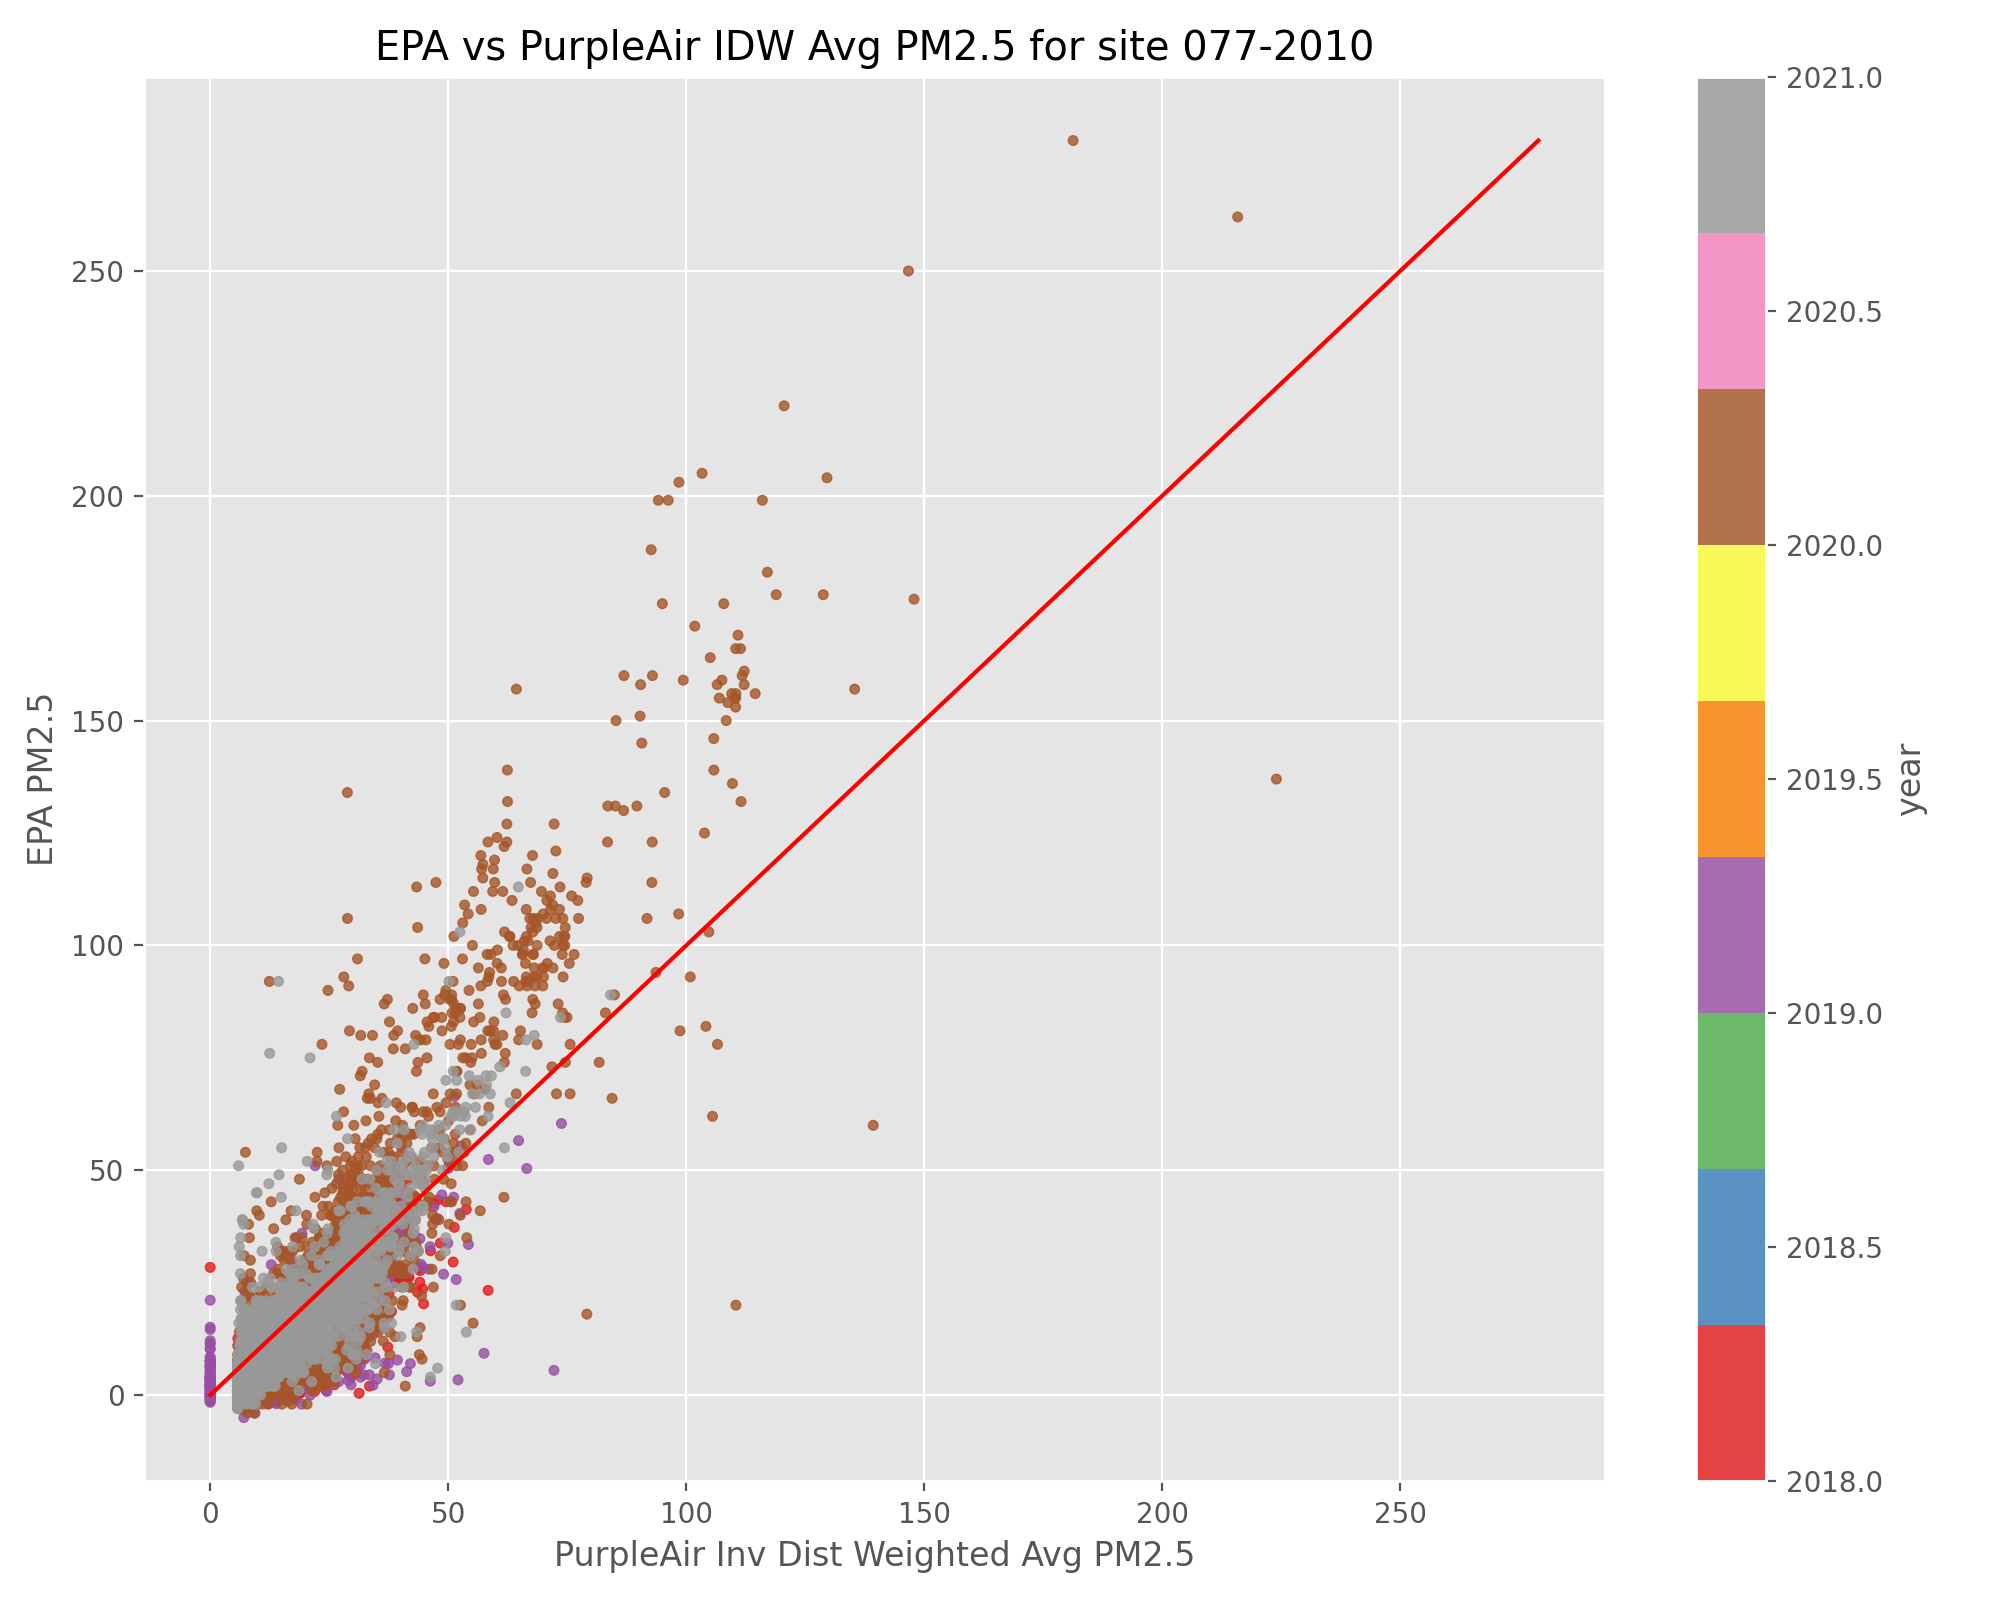
\includegraphics[width=0.8\textwidth]{appendix/site_plots/site-077-2010_epa-pa-hourly-plot.png}
\caption{Scatter plot comparing reported hourly PM2.5 measurements: the x-axis represents the IDW-weighted average of PurpleAir measurements, the y-axis represents reported NAAQS-primary monitor measurements. The red line is a 45$^\circ$ line, representing perfect correlation between the PurpleAir average and the NAAQS-primary monitor. This monitor is at site 2010 in county 077 (FIPS code).}
\label{fig:pa-epa-compare_077-2010}
\end{figure}
\begin{figure}
\centering
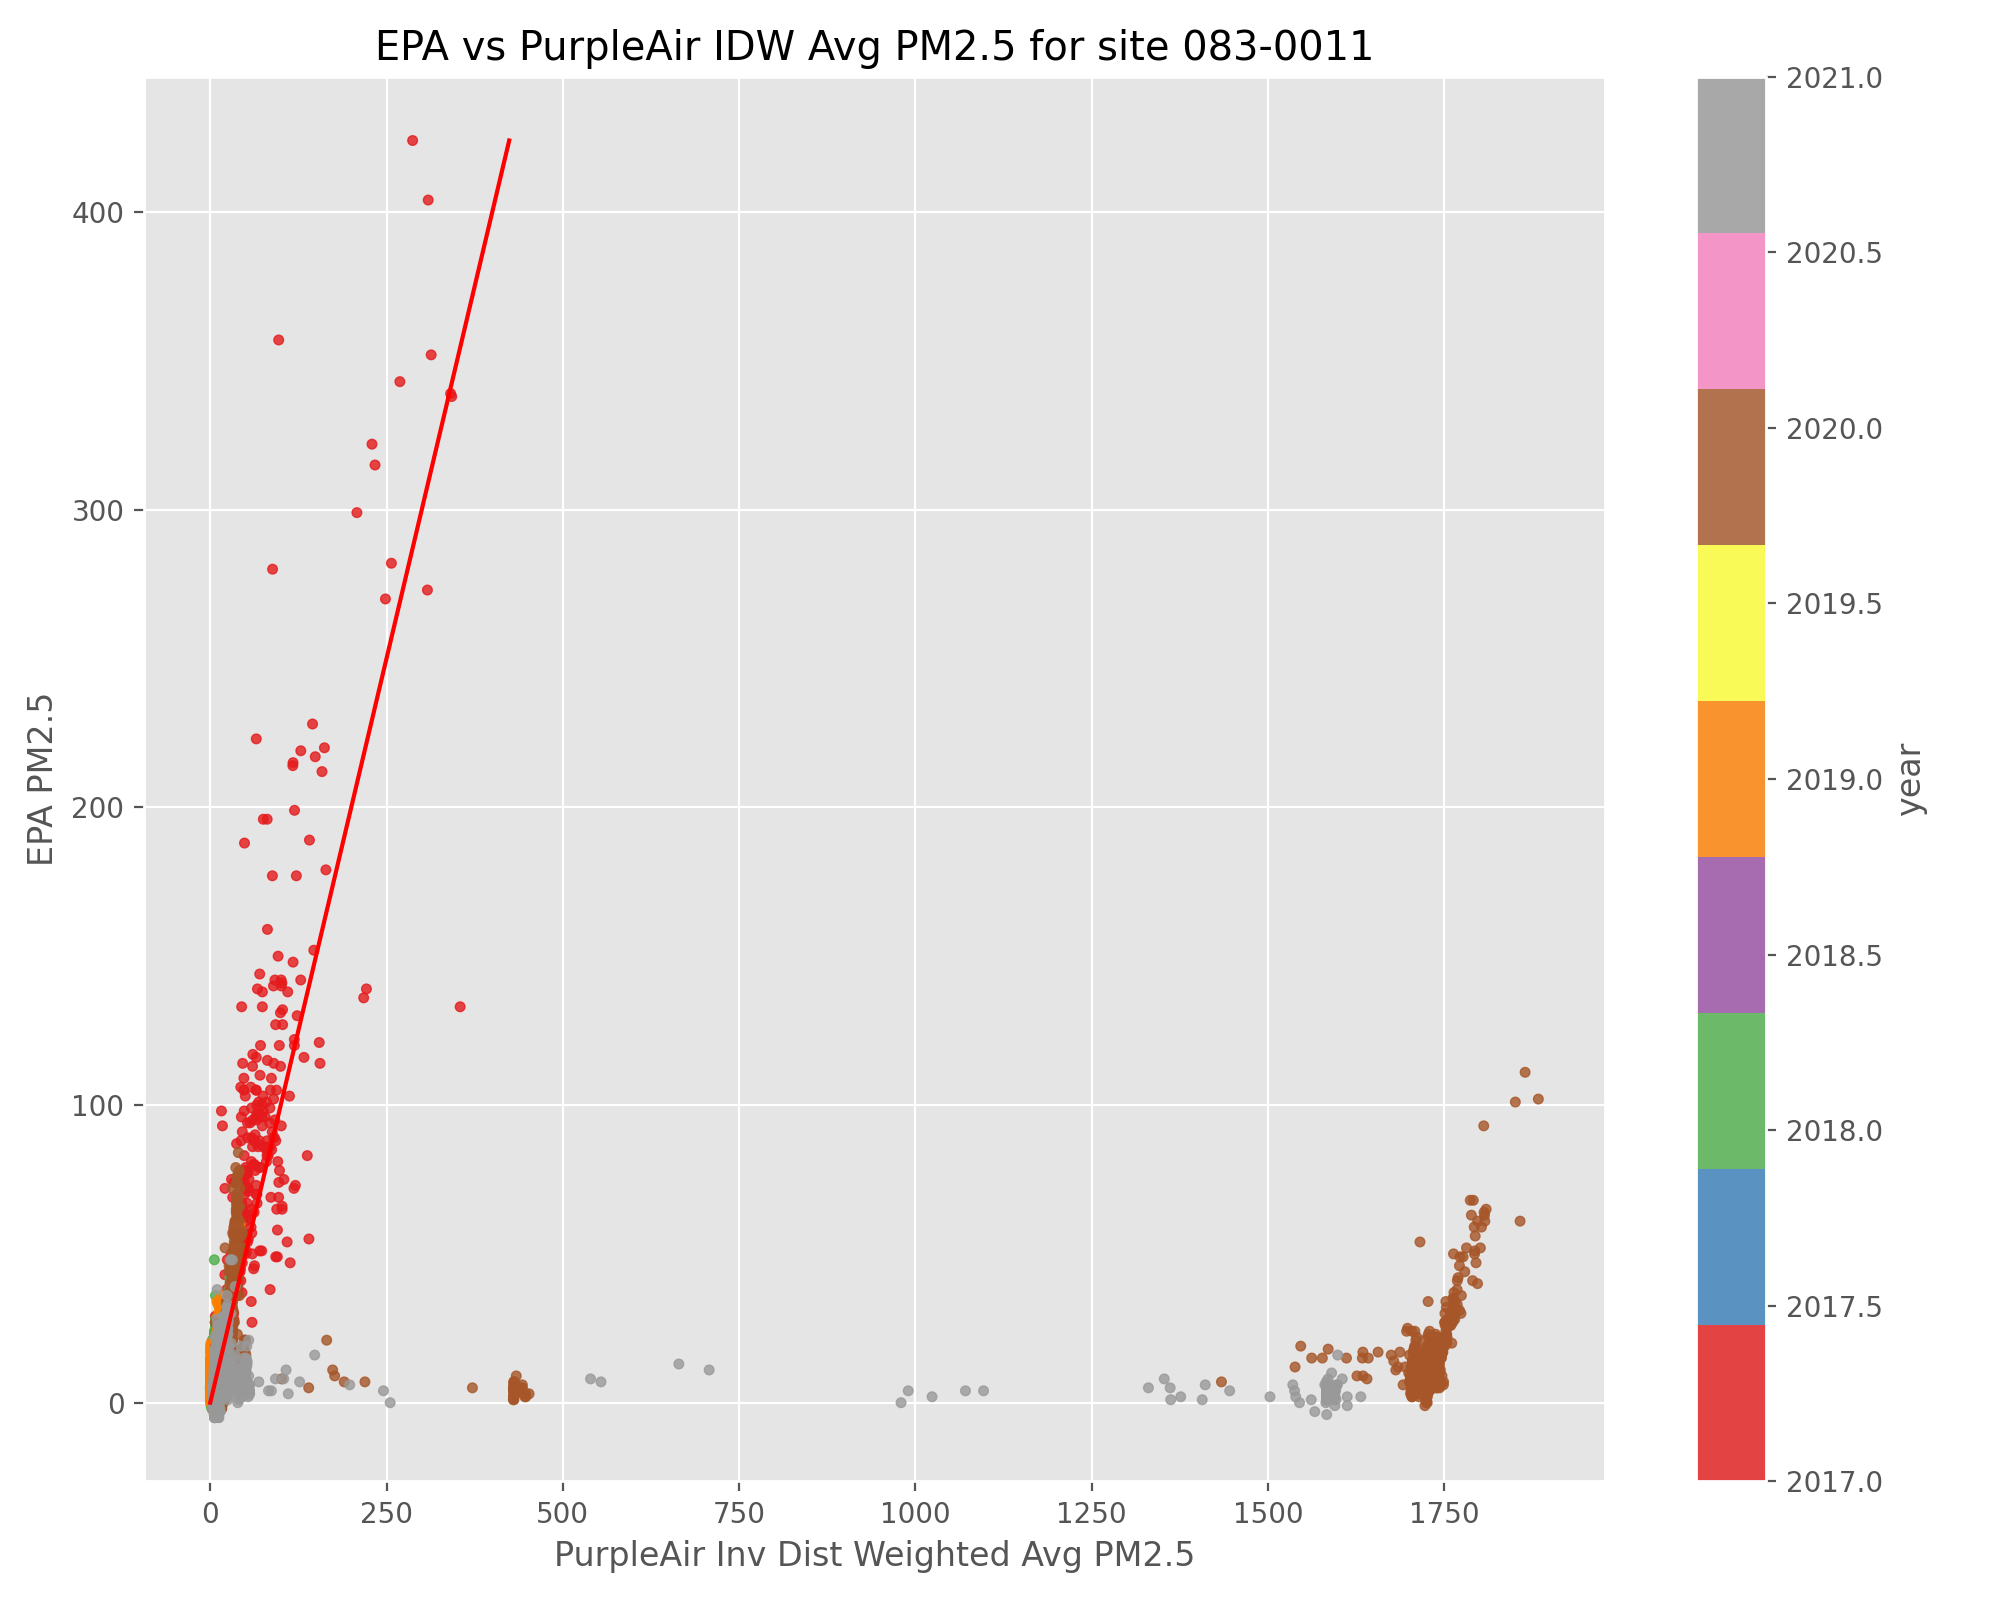
\includegraphics[width=0.8\textwidth]{appendix/site_plots/site-083-0011_epa-pa-hourly-plot.png}
\caption{Scatter plot comparing reported hourly PM2.5 measurements: the x-axis represents the IDW-weighted average of PurpleAir measurements, the y-axis represents reported NAAQS-primary monitor measurements. The red line is a 45$^\circ$ line, representing perfect correlation between the PurpleAir average and the NAAQS-primary monitor. This monitor is at site 0011 in county 083 (FIPS code).}
\label{fig:pa-epa-compare_083-0011}
\end{figure}
\begin{figure}
\centering
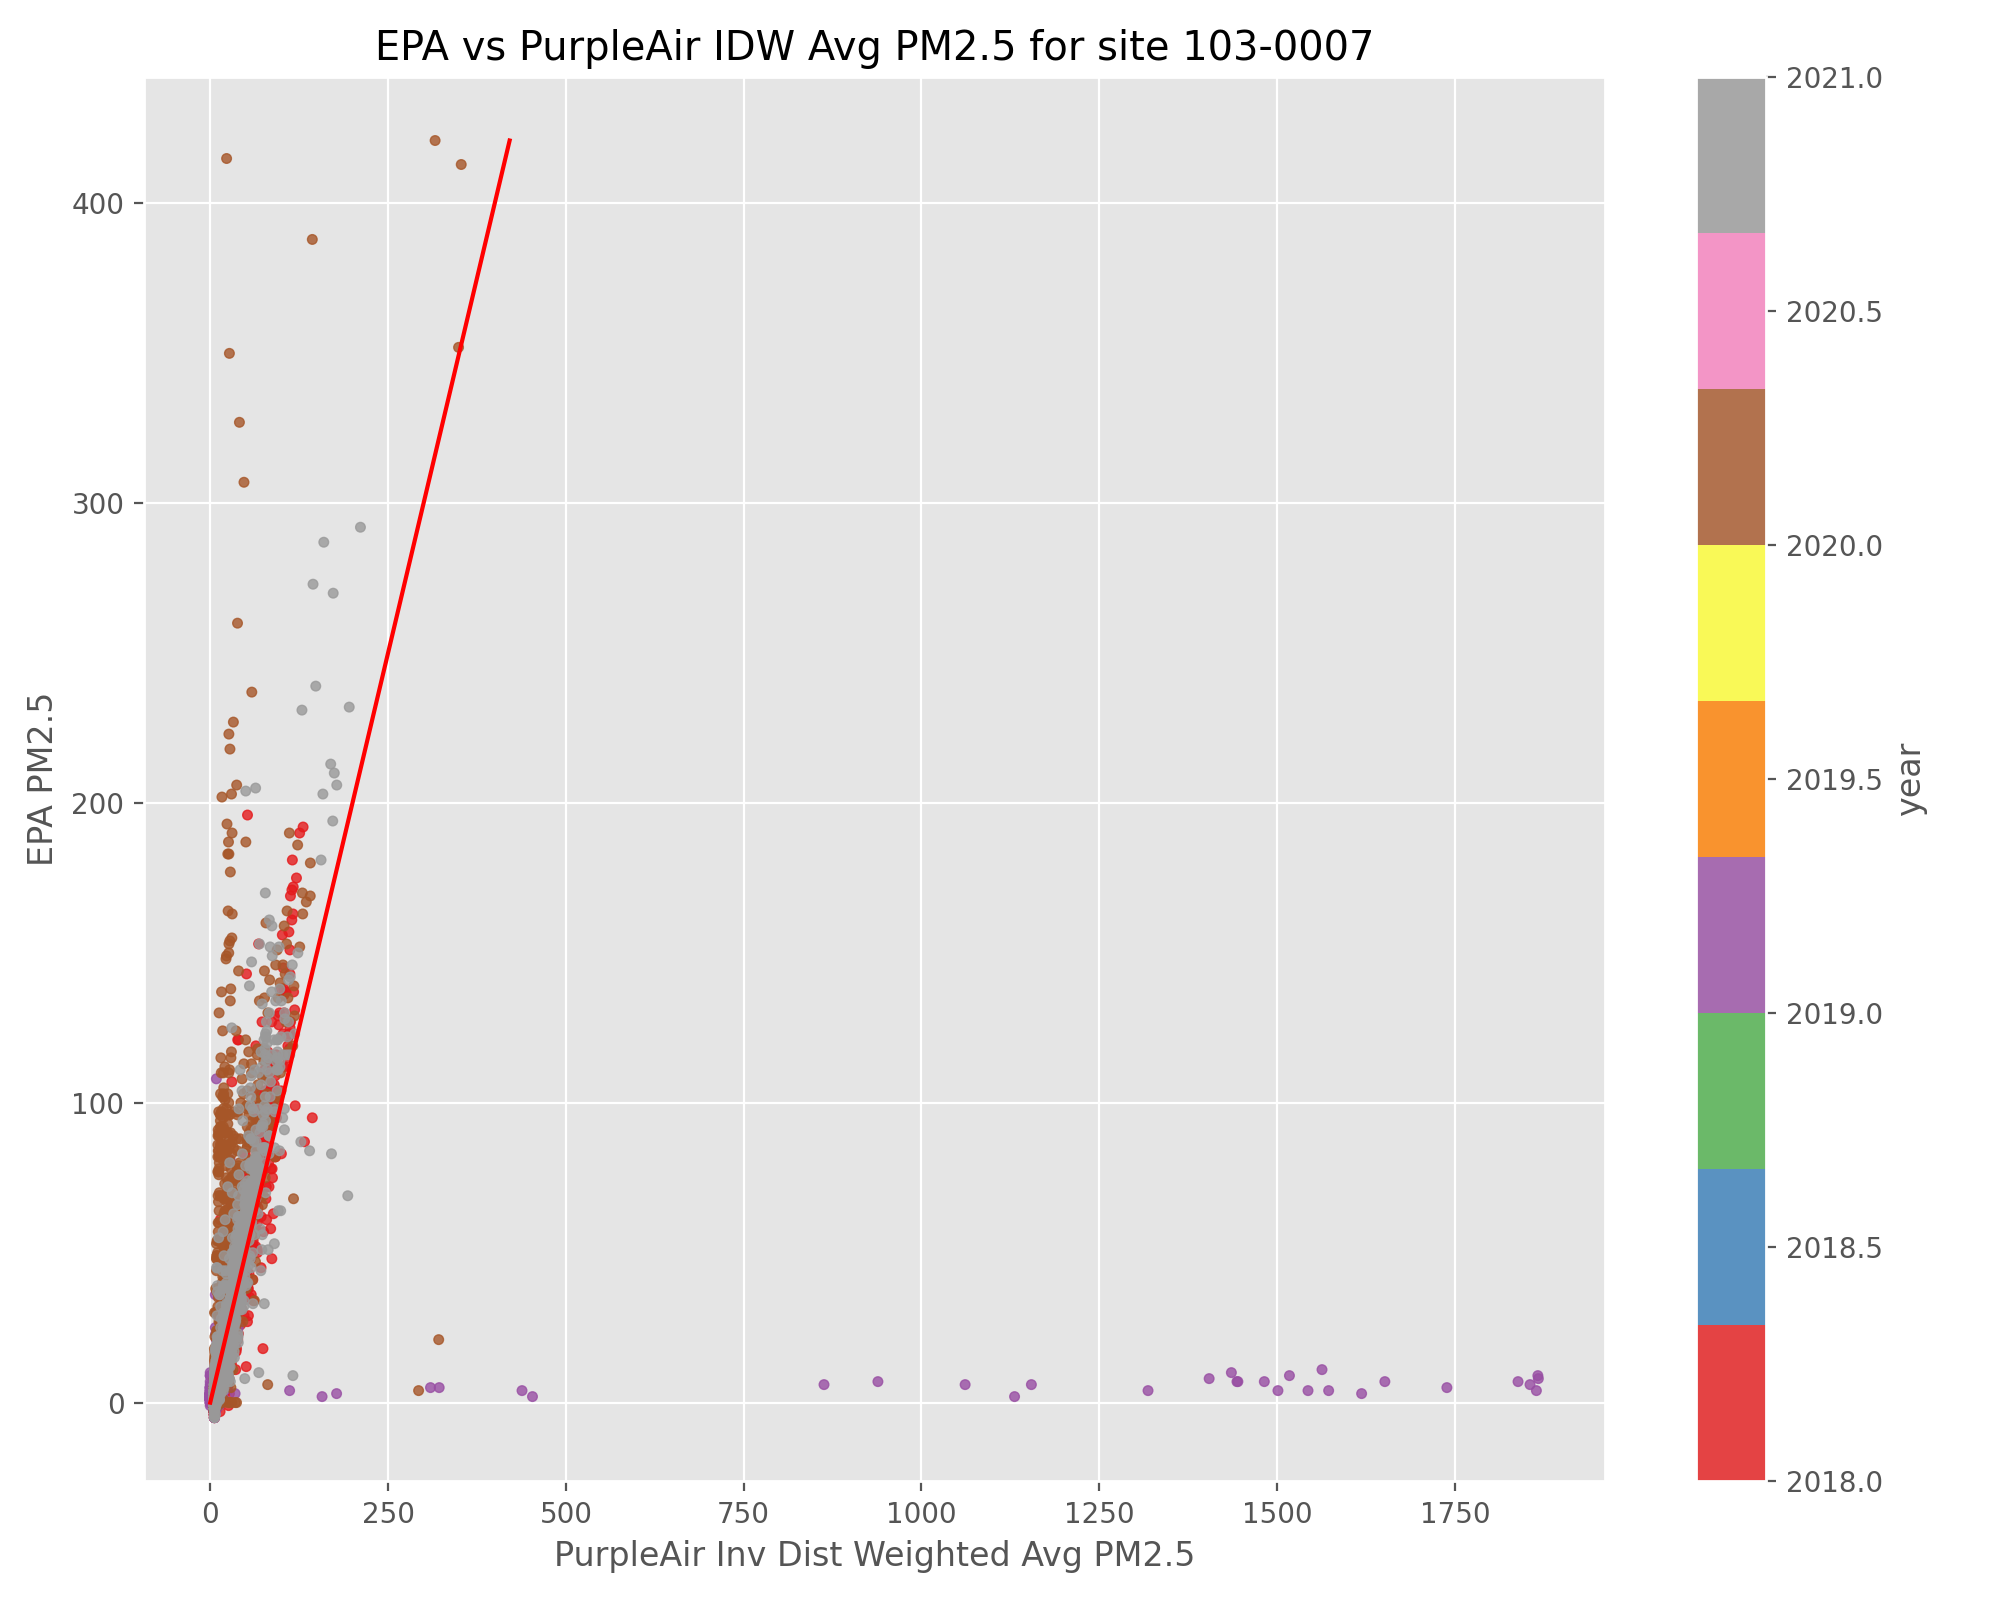
\includegraphics[width=0.8\textwidth]{appendix/site_plots/site-103-0007_epa-pa-hourly-plot.png}
\caption{Scatter plot comparing reported hourly PM2.5 measurements: the x-axis represents the IDW-weighted average of PurpleAir measurements, the y-axis represents reported NAAQS-primary monitor measurements. The red line is a 45$^\circ$ line, representing perfect correlation between the PurpleAir average and the NAAQS-primary monitor. This monitor is at site 0007 in county 103 (FIPS code).}
\label{fig:pa-epa-compare_103-0007}
\end{figure}
%=========================================
%  Kernel Density Comparison
%=========================================
\begin{figure}
\centering
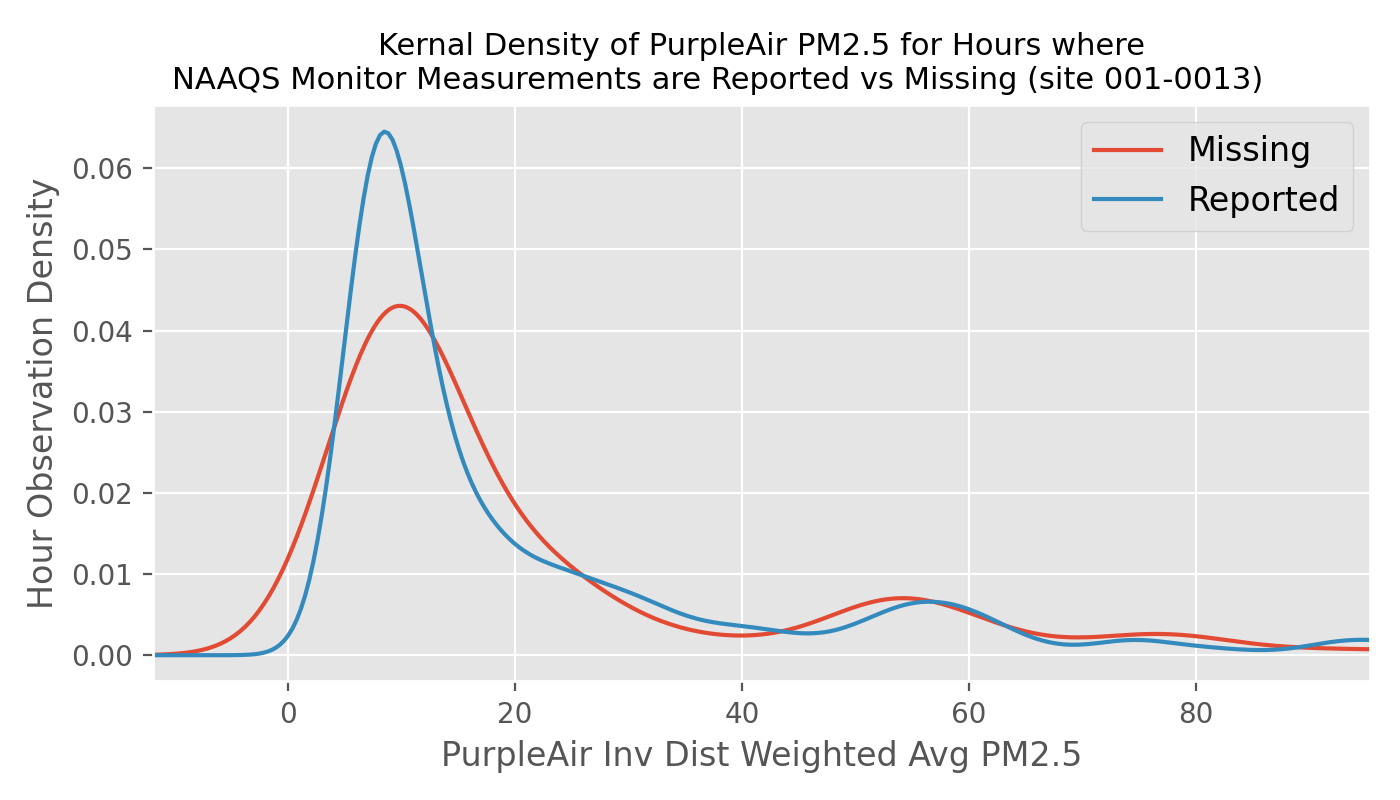
\includegraphics[width=0.8\textwidth]{appendix/site_plots/site-001-0013_epa-pa-missing-density.png}
\caption{Comparison of PM2.5 concentration densities for two sets of hours: reported (blue) and missing (red) hourly observations of the NAAQS monitor. Both densities use the hourly PurpleAir PM2.5 concentration estimates for this site, calculated using the IDW average of PurpleAir sensors within 5 miles of the NAAQS monitor location. This monitor is at site 0013 in county 001 (FIPS code).}
\label{fig:missing-density_001-0013}
\end{figure}






\begin{figure}
\centering
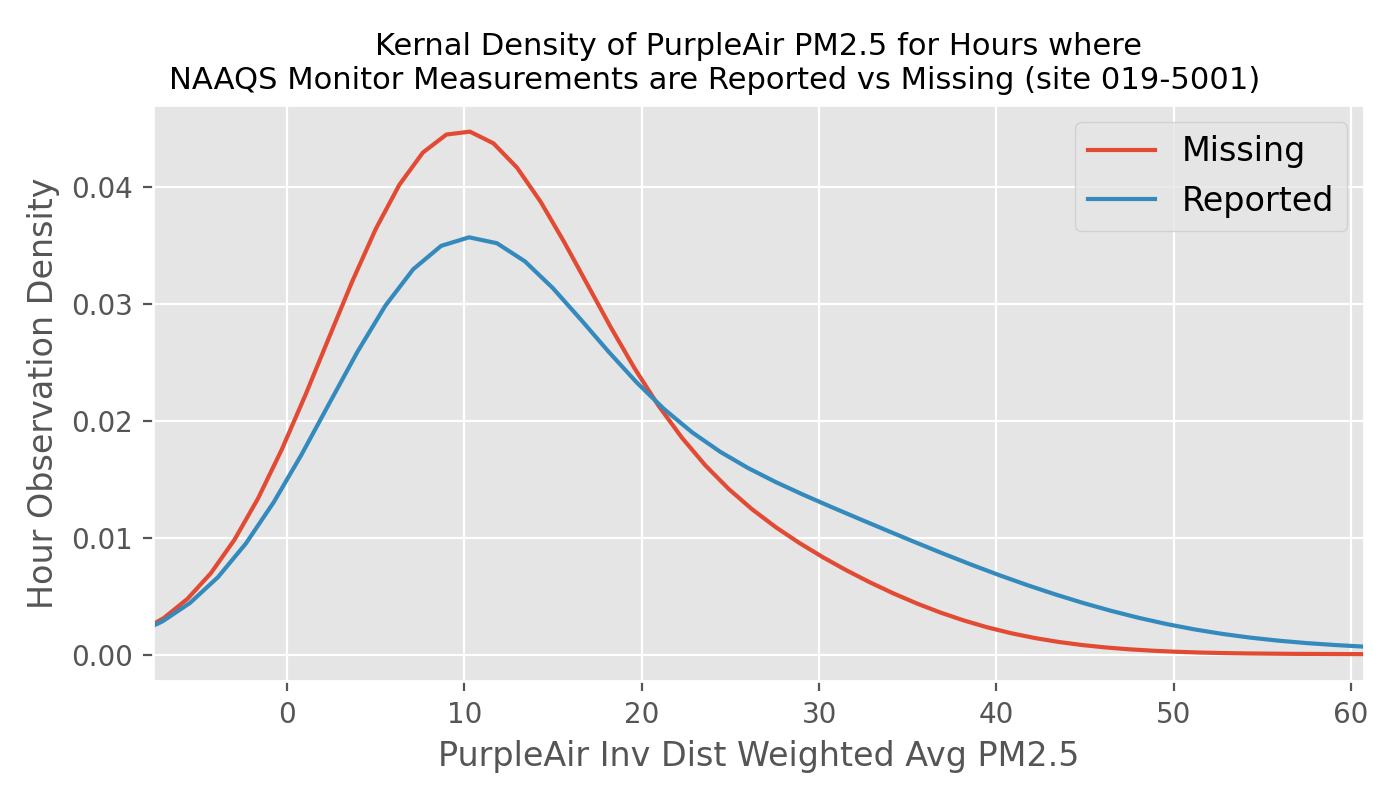
\includegraphics[width=0.8\textwidth]{appendix/site_plots/site-019-5001_epa-pa-missing-density.png}
\caption{Comparison of PM2.5 concentration densities for two sets of hours: reported (blue) and missing (red) hourly observations of the NAAQS monitor. Both densities use the hourly PurpleAir PM2.5 concentration estimates for this site, calculated using the IDW average of PurpleAir sensors within 5 miles of the NAAQS monitor location. This monitor is at site 5001 in county 019 (FIPS code).}
\label{fig:missing-density_019-5001}
\end{figure}

\begin{figure}
\centering
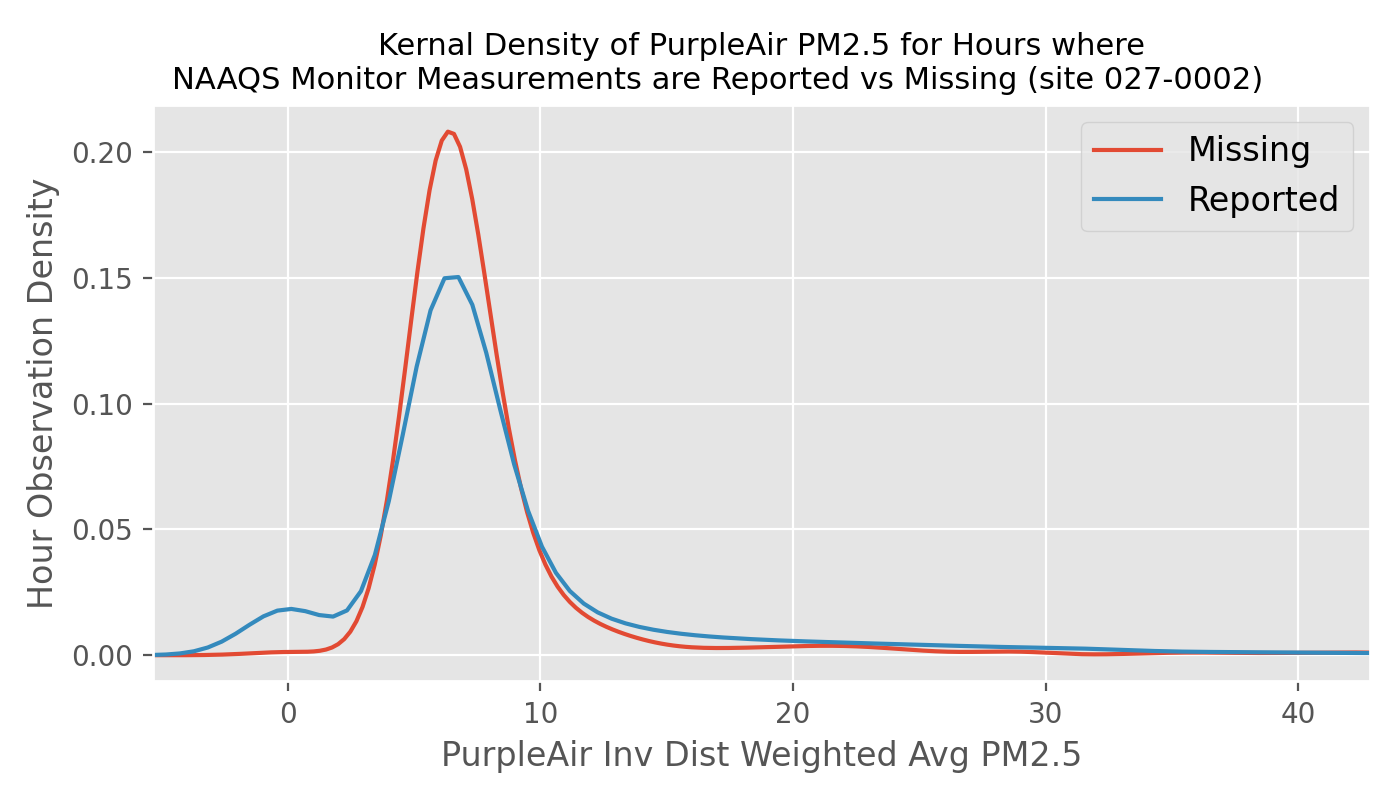
\includegraphics[width=0.8\textwidth]{appendix/site_plots/site-027-0002_epa-pa-missing-density.png}
\caption{Comparison of PM2.5 concentration densities for two sets of hours: reported (blue) and missing (red) hourly observations of the NAAQS monitor. Both densities use the hourly PurpleAir PM2.5 concentration estimates for this site, calculated using the IDW average of PurpleAir sensors within 5 miles of the NAAQS monitor location. This monitor is at site 0002 in county 027 (FIPS code).}
\label{fig:missing-density_027-0002}
\end{figure}

\begin{figure}
\centering
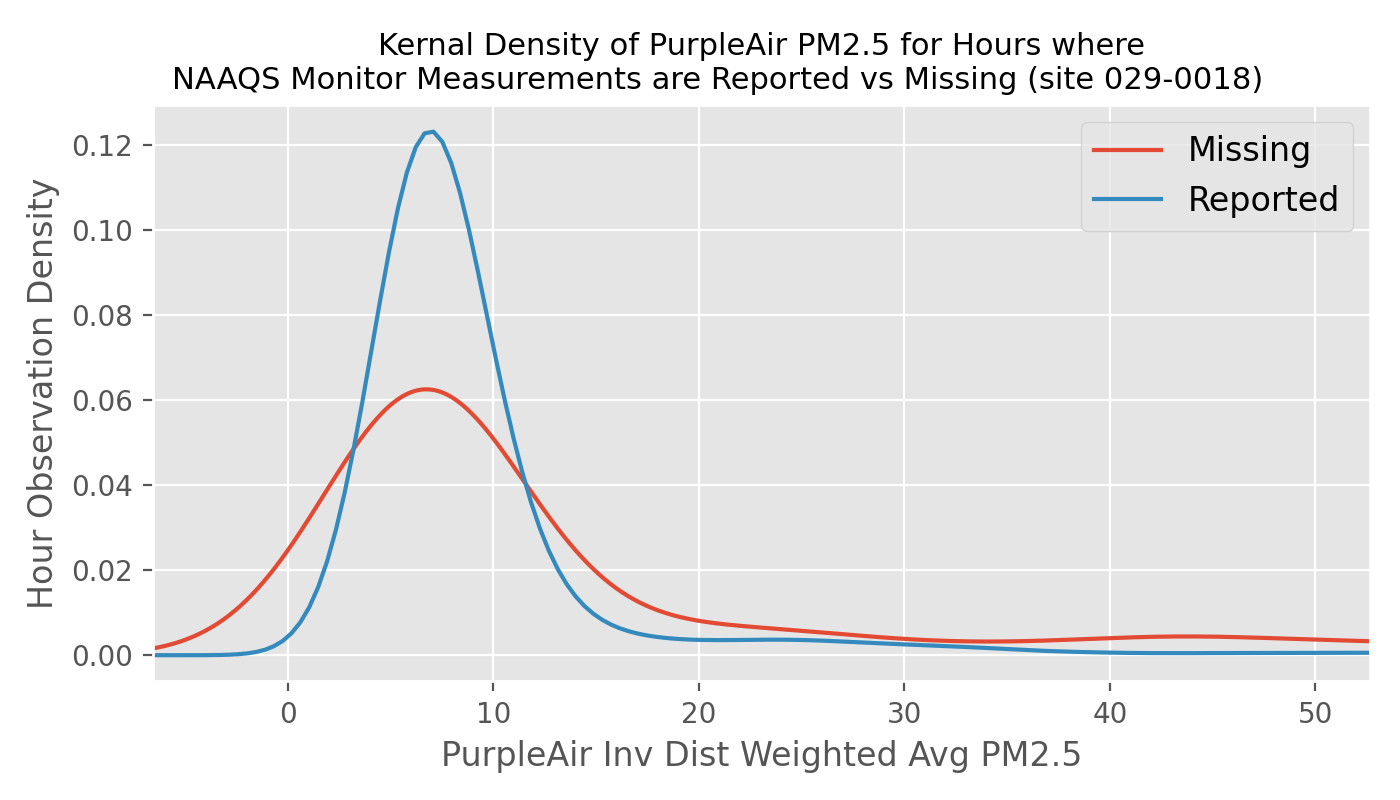
\includegraphics[width=0.8\textwidth]{appendix/site_plots/site-029-0018_epa-pa-missing-density.png}
\caption{Comparison of PM2.5 concentration densities for two sets of hours: reported (blue) and missing (red) hourly observations of the NAAQS monitor. Both densities use the hourly PurpleAir PM2.5 concentration estimates for this site, calculated using the IDW average of PurpleAir sensors within 5 miles of the NAAQS monitor location. This monitor is at site 0018 in county 029 (FIPS code).}
\label{fig:missing-density_029-0018}
\end{figure}

\begin{figure}
\centering
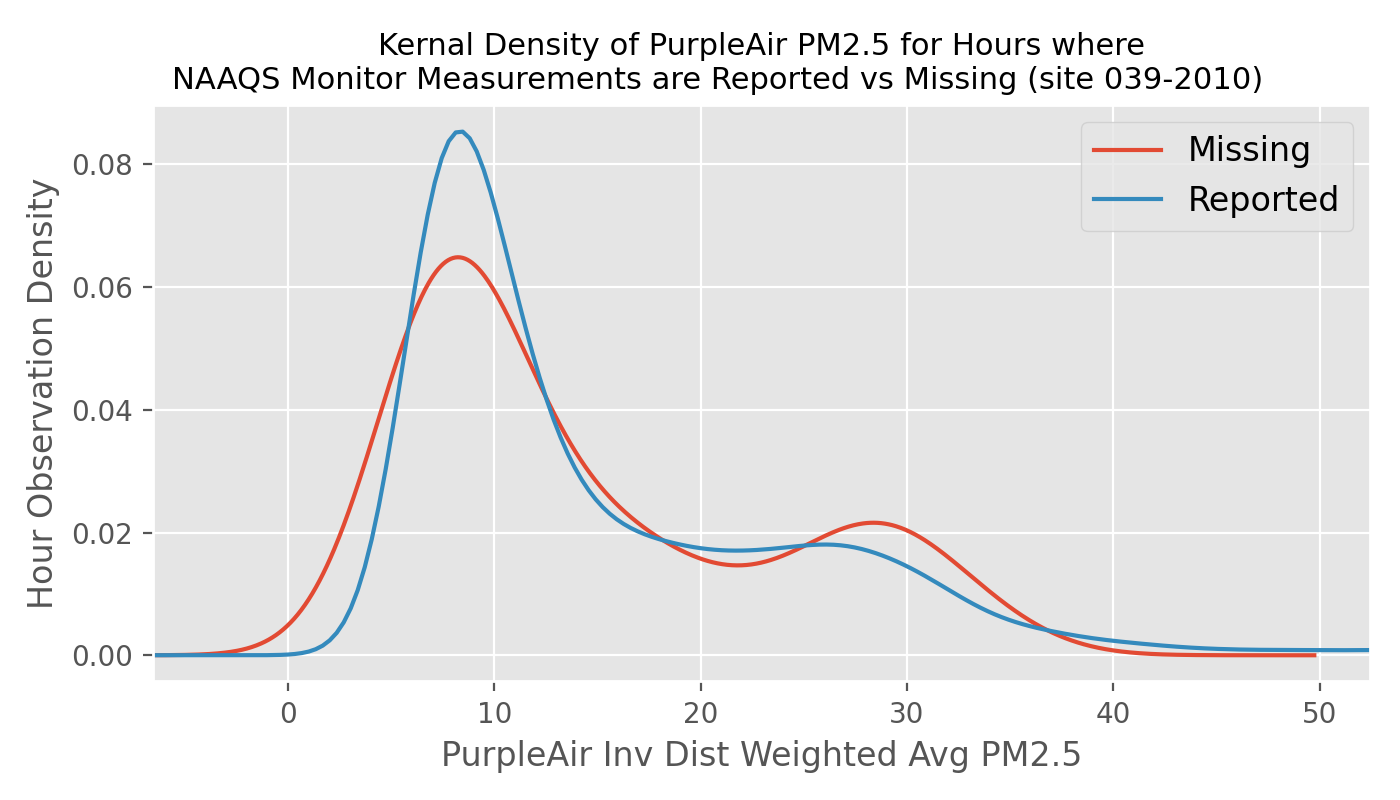
\includegraphics[width=0.8\textwidth]{appendix/site_plots/site-039-2010_epa-pa-missing-density.png}
\caption{Comparison of PM2.5 concentration densities for two sets of hours: reported (blue) and missing (red) hourly observations of the NAAQS monitor. Both densities use the hourly PurpleAir PM2.5 concentration estimates for this site, calculated using the IDW average of PurpleAir sensors within 5 miles of the NAAQS monitor location. This monitor is at site 2010 in county 039 (FIPS code).}
\label{fig:missing-density_039-2010}
\end{figure}

\begin{figure}
\centering
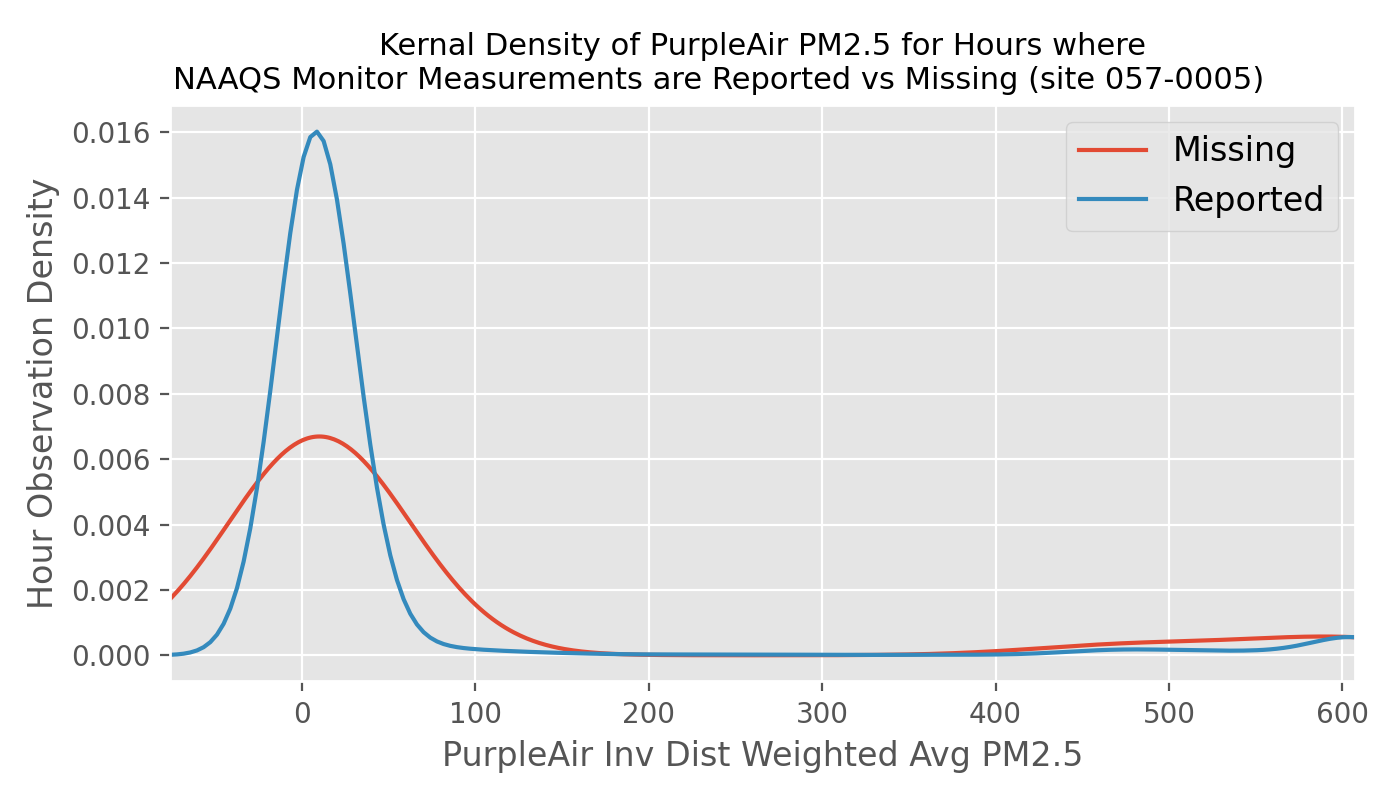
\includegraphics[width=0.8\textwidth]{appendix/site_plots/site-057-0005_epa-pa-missing-density.png}
\caption{Comparison of PM2.5 concentration densities for two sets of hours: reported (blue) and missing (red) hourly observations of the NAAQS monitor. Both densities use the hourly PurpleAir PM2.5 concentration estimates for this site, calculated using the IDW average of PurpleAir sensors within 5 miles of the NAAQS monitor location. This monitor is at site 0005 in county 057 (FIPS code).}
\label{fig:missing-density_057-0005}
\end{figure}

\begin{figure}
\centering
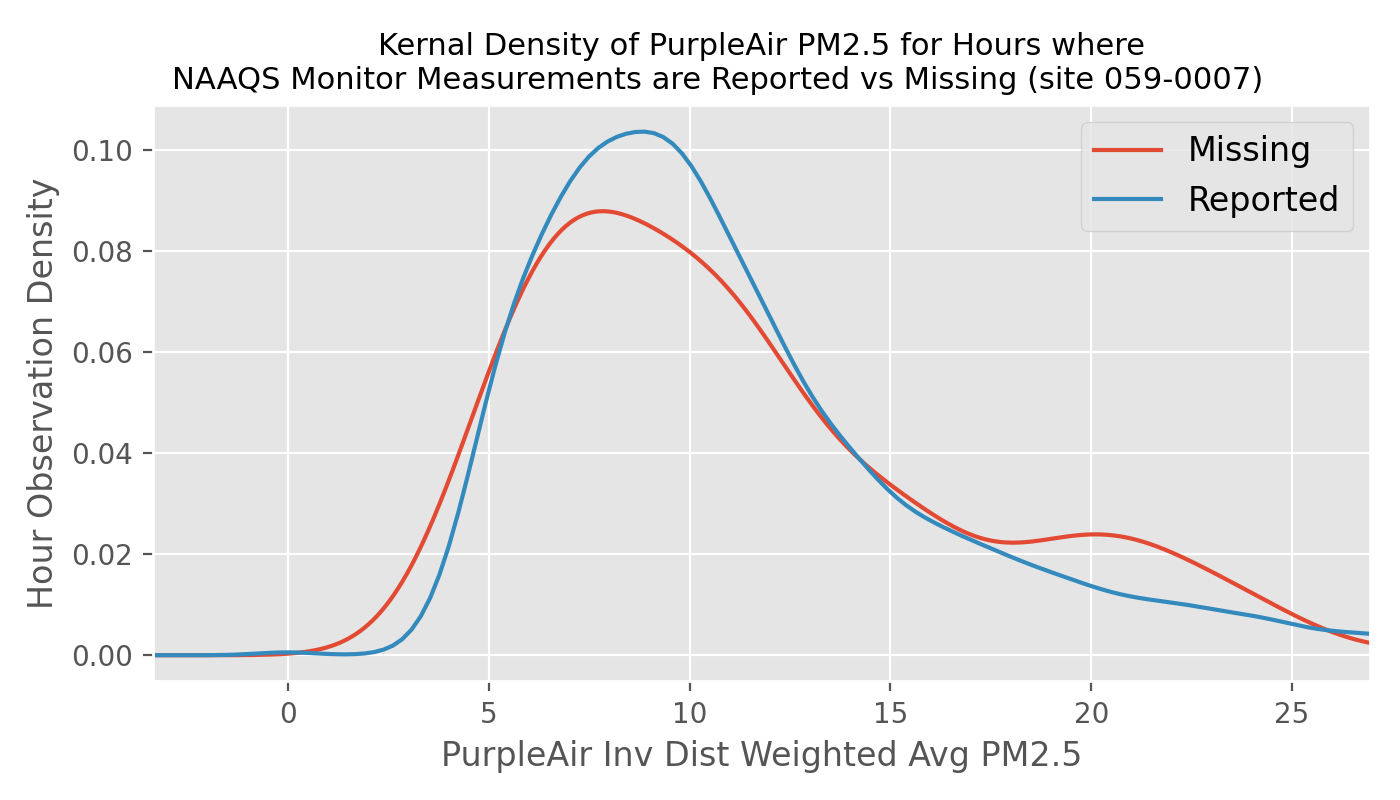
\includegraphics[width=0.8\textwidth]{appendix/site_plots/site-059-0007_epa-pa-missing-density.png}
\caption{Comparison of PM2.5 concentration densities for two sets of hours: reported (blue) and missing (red) hourly observations of the NAAQS monitor. Both densities use the hourly PurpleAir PM2.5 concentration estimates for this site, calculated using the IDW average of PurpleAir sensors within 5 miles of the NAAQS monitor location. This monitor is at site 0007 in county 059 (FIPS code).}
\label{fig:missing-density_059-0007}
\end{figure}

\begin{figure}
\centering
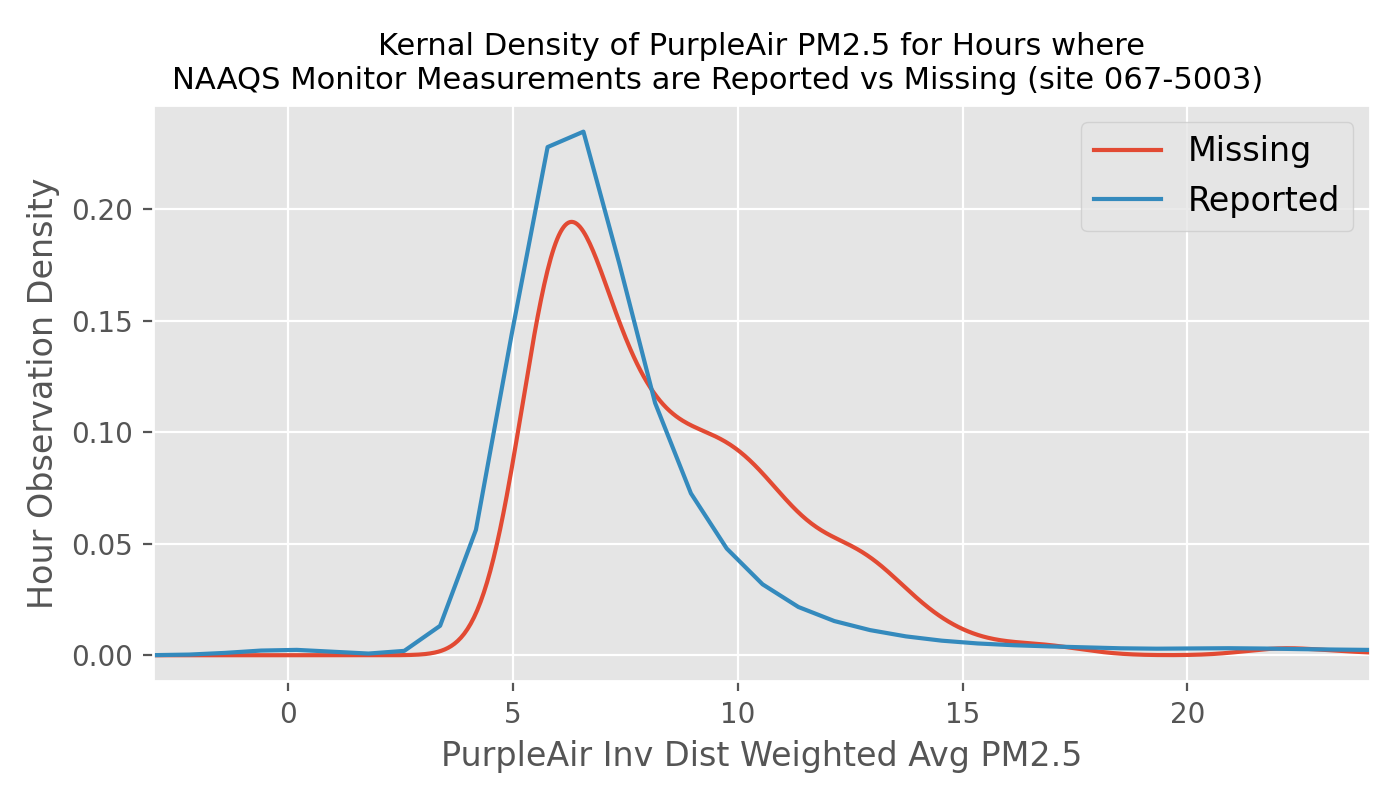
\includegraphics[width=0.8\textwidth]{appendix/site_plots/site-067-5003_epa-pa-missing-density.png}
\caption{Comparison of PM2.5 concentration densities for two sets of hours: reported (blue) and missing (red) hourly observations of the NAAQS monitor. Both densities use the hourly PurpleAir PM2.5 concentration estimates for this site, calculated using the IDW average of PurpleAir sensors within 5 miles of the NAAQS monitor location. This monitor is at site 5003 in county 067 (FIPS code).}
\label{fig:missing-density_067-5003}
\end{figure}

\begin{figure}
\centering
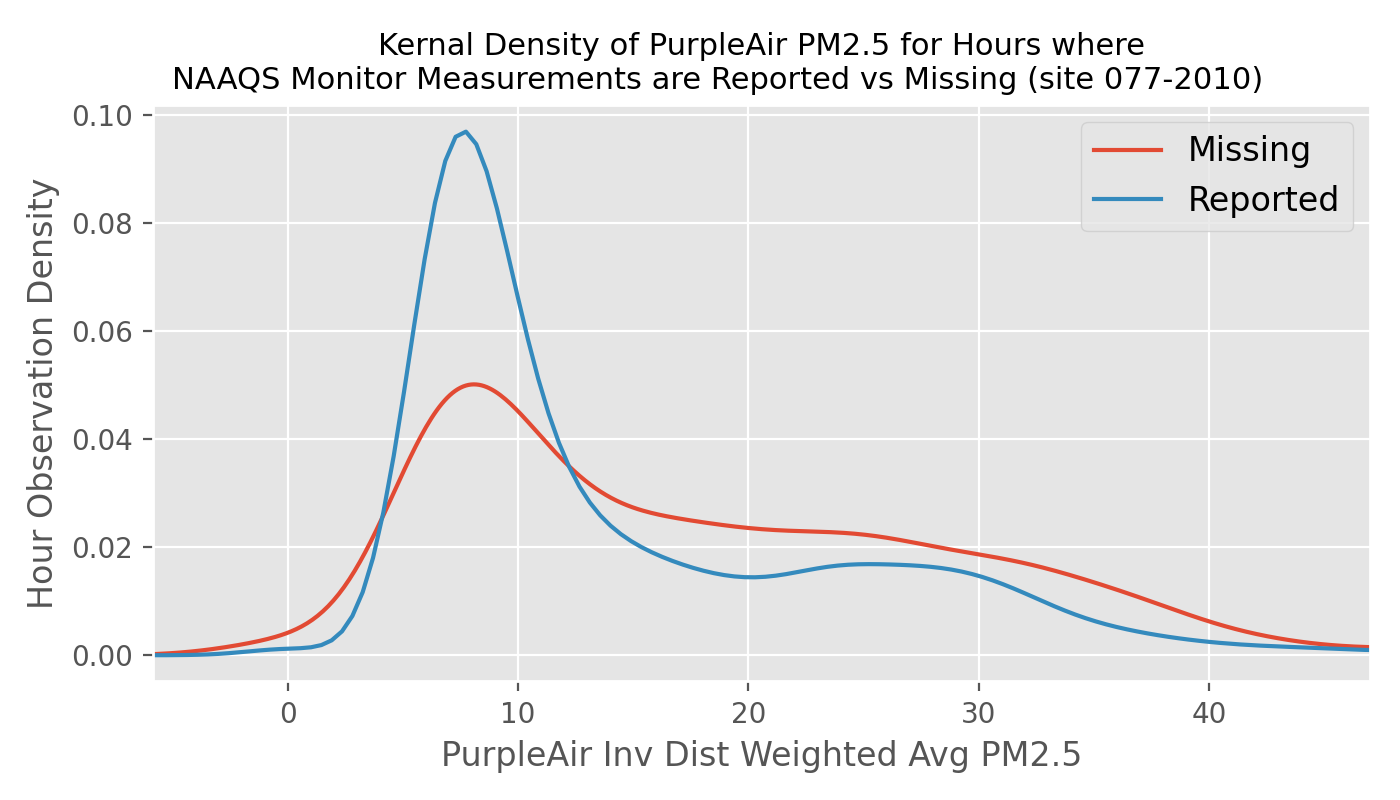
\includegraphics[width=0.8\textwidth]{appendix/site_plots/site-077-2010_epa-pa-missing-density.png}
\caption{Comparison of PM2.5 concentration densities for two sets of hours: reported (blue) and missing (red) hourly observations of the NAAQS monitor. Both densities use the hourly PurpleAir PM2.5 concentration estimates for this site, calculated using the IDW average of PurpleAir sensors within 5 miles of the NAAQS monitor location. This monitor is at site 2010 in county 077 (FIPS code).}
\label{fig:missing-density_077-2010}
\end{figure}

\begin{figure}
\centering
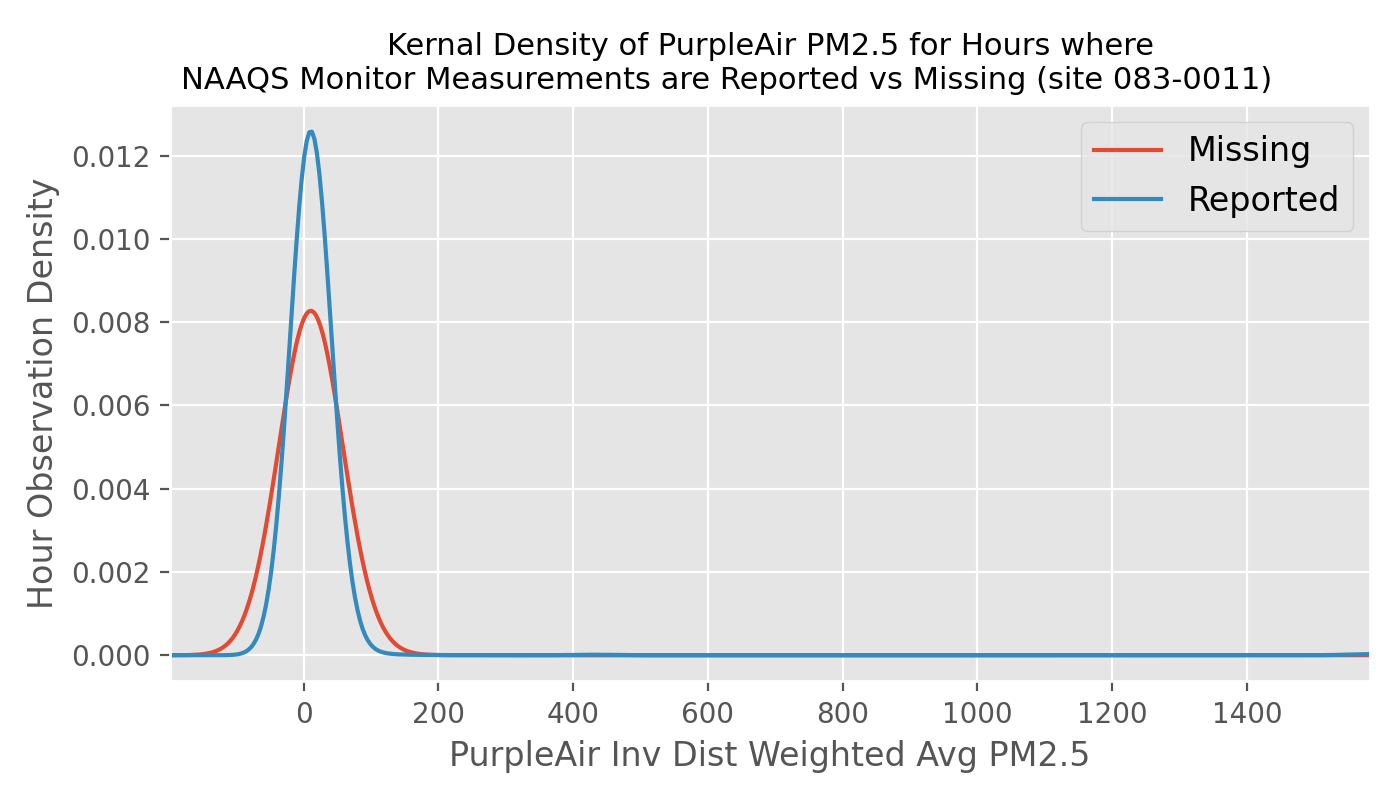
\includegraphics[width=0.8\textwidth]{appendix/site_plots/site-083-0011_epa-pa-missing-density.png}
\caption{Comparison of PM2.5 concentration densities for two sets of hours: reported (blue) and missing (red) hourly observations of the NAAQS monitor. Both densities use the hourly PurpleAir PM2.5 concentration estimates for this site, calculated using the IDW average of PurpleAir sensors within 5 miles of the NAAQS monitor location. This monitor is at site 0011 in county 083 (FIPS code).}
\label{fig:missing-density_083-0011}
\end{figure}

\begin{figure}
\centering
\includegraphics[width=0.8\textwidth]{appendix/site_plots/site-103-0007_epa-pa-missing-density.png}
\caption{Comparison of PM2.5 concentration densities for two sets of hours: reported (blue) and missing (red) hourly observations of the NAAQS monitor. Both densities use the hourly PurpleAir PM2.5 concentration estimates for this site, calculated using the IDW average of PurpleAir sensors within 5 miles of the NAAQS monitor location. This monitor is at site 0007 in county 103 (FIPS code).}
\label{fig:missing-density_103-0007}
\end{figure}

